\documentclass[aspectratio=169,usenames,dvipsnames]{beamer}

% fonts
%\usepackage[T1]{fontenc}
%\usepackage[utf8]{inputenc}

%\usefonttheme{professionalfonts} % using non standard fonts for beamer
\usefonttheme{serif} % default family is serif

\usepackage{palatino}
%\usepackage{gfsartemisia}
%\usepackage{theanooldstyle}

\usepackage{euscript}	 % Шрифт Евклид
\usepackage{mathrsfs} % Красивый матшрифт
\usepackage{amssymb}
\usepackage{bm}
\usepackage{calc} % perform arithmetic on the arguments
\usepackage{cancel} % cancelling things
\usepackage{marvosym} % fancy arrow
\usepackage[ruled,vlined]{algorithm2e}
\usepackage{algorithmic}

\definecolor{mygreen}{HTML}{348A41}  % 53945D
\definecolor{myred}{HTML}{B73239} 
\definecolor{myorange}{HTML}{AB5F1F}  % 805129
\definecolor{mypurple}{HTML}{533E8F} 
\definecolor{myblack}{HTML}{4C4848} 
\definecolor{mygrey}{HTML}{F4EDE0} %  F5F1EA

\usepackage{epstopdf}
\usepackage{xcolor}

% adding images
\usepackage{graphicx} 
\usepackage{tcolorbox}

% adding gifs
\usepackage{animate}

% positioning textblocks
\usepackage[absolute, overlay]{textpos} 
\textblockorigin{0mm}{0mm} % start everything near the top-left corner

% Работа с русским языком
\usepackage{cmap}					% поиск в PDF
%\usepackage{mathtext} 				% русские буквы в фомулах
%\usepackage[T2A]{fontenc}			% кодировка
%\usepackage[utf8]{inputenc}			% кодировка исходного текста

% Дополнительная работа с математикой
%\usepackage{amsmath,amsfonts,amssymb,amsthm,mathtools} % AMS
%\usepackage{icomma} % "Умная" запятая: $0,2$ --- число, $0, 2$ --- перечисление

%% Номера формул
%\mathtoolsset{showonlyrefs=true} % Показывать номера только у тех формул, на которые есть \eqref{} в тексте.

% Работа с картинками
\usepackage{graphicx}  % Для вставки рисунков
\graphicspath{{images/}}  % папки с картинками
\usepackage{wrapfig} % Обтекание рисунков и таблиц текстом

% drawing with tikz
\usepackage{tikz}
\usepackage{hf-tikz}
\usetikzlibrary{arrows}
\usetikzlibrary{shapes}
\usetikzlibrary{plotmarks}

\tikzset{
	treenode/.style = {align=center, inner sep=1.ex, minimum size=1cm,
		font=\sffamily},
	arn_n/.style = {treenode, rectangle, black, draw=black, minimum width = 0.05\textwidth, minimum height = 1 cm},% 
	level distance = 2.5cm,
	level 1/.style={sibling distance=16.cm},
	level 2/.style={sibling distance=8.cm},
	level 3/.style={sibling distance=3.7cm}
}

  \tikzset{
	invisible/.style={opacity=0},
	visible on/.style={alt=#1{}{invisible}},
	alt/.code args={<#1>#2#3}{%
		\alt<#1>{\pgfkeysalso{#2}}{\pgfkeysalso{#3}} % \pgfkeysalso doesn't change the path
	},
}

%% Работа с таблицами
%\usepackage{array,tabularx,tabulary,booktabs} % Дополнительная работа с таблицами
%\usepackage{longtable}  % Длинные таблицы
%\usepackage{multirow} % Слияние строк в таблице
%\renewcommand{\arraystretch}{1.3} %The height of each row is set to 1.5 relative to its default height. 

% Two ways of getting rid of total slides number

%\setbeamertemplate{footline}
%    {\begin{beamercolorbox}[sep=1ex]{author in head/foot}
%      \rlap{\textit{\insertshorttitle}}\hfill\insertauthor\hfill\llap{\insertframenumber}%
%      \end{beamercolorbox}%
%}

\makeatletter
\setbeamertemplate{footline}
{
	\leavevmode%
	\hbox{%
		\begin{beamercolorbox}[wd=.333333\paperwidth,ht=2.25ex,dp=1ex,center]{author in head/foot}%
			\usebeamerfont{author in head/foot}\insertshortauthor~~\beamer@ifempty{\insertshortinstitute}{}{(\insertshortinstitute)}
		\end{beamercolorbox}%
		\begin{beamercolorbox}[wd=.333333\paperwidth,ht=2.25ex,dp=1ex,center]{title in head/foot}%
			\usebeamerfont{title in head/foot}\insertshorttitle
		\end{beamercolorbox}%
		\begin{beamercolorbox}[wd=.333333\paperwidth,ht=2.25ex,dp=1ex,right]{date in head/foot}%
			\usebeamerfont{date in head/foot}\insertshortdate\hspace*{2em}
			\insertframenumber/\inserttotalframenumber\hspace*{2ex} 
	\end{beamercolorbox}}%
	\vskip0pt%
}
\makeatother

% Beamer presentation style
\mode<presentation> {
	\usetheme{Pittsburgh}
	\usecolortheme{dove}
	%\setbeamertemplate{footline} % To remove the footer line in all slides uncomment this line
	%\setbeamertemplate{footline}[page number] % To replace the footer line in all slides with a simple slide count uncomment this line
	%\setbeamertemplate{navigation symbols}{} % To remove the navigation symbols from the bottom of all slides uncomment this line
	
	%	\setbeamercolor{frametitle}{fg=white,bg=greyone}
	%	\setbeamercolor{titlelike}{parent=palette quaternary}
	
	%	\setbeamertemplate{frametitle}
	%	{
	%		\begin{textblock*}{\hsize}(.75\hsize,0.05\vsize)
	%			\begin{tcolorbox}[colframe=white, colback=mygrey, width=0.33\hsize,
	%				arc=2.mm, boxsep=2mm,
	%				box align=center,
	%				halign=center,
	%				valign=center,
	%				]
	%				\insertframetitle
	%			\end{tcolorbox}
	%		\end{textblock*}
	%	}
}

%% custom title
%\newcommand{\myframetitle}[3]{
%	\begin{textblock*}{\hsize}(#1,0.05\vsize)
%		\begin{tcolorbox}[colframe=white, colback=mygrey, width=#2,
%			arc=2.mm, boxsep=2mm,
%			box align=center,
%			halign=center,
%			valign=center,
%			]
%			\Large
%			#3
%		\end{tcolorbox}
%	\end{textblock*}
%}

% custom title
\newcommand{\myframetitle}[3]{
	\begin{textblock*}{#1}(#2,0.05\vsize)
		\begin{tcolorbox}[colframe=white, colback=mygrey, width=#1,
			arc=2.mm, boxsep=2mm,
			box align=center,
			halign=center,
			valign=center,
			]
			\Large
			\centering
			#3
		\end{tcolorbox}
	\end{textblock*}
}

% custom subtitle
\newcommand{\myframesubtitle}[2]{
	
	\begin{textblock*}{5cm}(#1,0.123\vsize)
		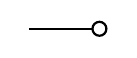
\begin{tikzpicture}
		\draw[thick,-o,black] (0.,0.) -- (1.0,0.);
		\end{tikzpicture}
	\end{textblock*}
	
	\begin{textblock*}{0.5\hsize}(#1+0.075\paperwidth,0.1\vsize)
		\normalsize
		\vspace{0.6mm}
		%		\centering
		#2
	\end{textblock*}
}

% new color for the bullet/subbullet
\newcommand{\mybullet}{$\textcolor{myblack}{\bullet}$}
\newcommand{\mysubbullet}{$\textcolor{myblack}{\circ}$}
\newcommand{\ev}{\mathbb{E}_{\text{p}(\bm x,y)}}
\newcommand{\pluseq}{\mathrel{+}=}

%\title{Introduction to Machine Learning\\
%Lecture 1}
%\author[name]{Oleg Filatov \inst{1} \and   Zakharov \inst{2}}%
%\institute{
%	\inst{1} DESY 
%	\inst{2} Novosibirsk State University
%	\newline
%	\vspace{1em}
%	
%%	\includegraphics[width=1.1cm]{CMS_logo.pdf}\hspace*{0.4cm}
%	
\includegraphics[width=1.1cm]{DESY_logo.png}\hspace*{0.4cm}
%	\includegraphics[width=2.1cm]{NSU_logo.png}\hspace*{0.4cm}
%}
%
%\date{}

%----------------------------------------------------------------------------------------
%	TITLE PAGE
%----------------------------------------------------------------------------------------

\author[Olga Razuvaeva]{Olga Razuvaeva\inst{1, 2}, Sergey Korpachev\inst{3, 4}, Stepan Zakharov\inst{5}}%
\institute[ITEP, MEPhI]{
	\newline
	\inst{1} {Institute for Theoretical and Experimental Physics}\\
	\vspace{1mm}
	\inst{2} {National Research Nuclear University MEPhI (Moscow Engineering Physics Institute)}\\
	\vspace{1mm}
	\inst{3} {Moscow Institute of Physics and Technology}\\
	\vspace{1mm}
	\inst{4} {Lebedev Physical Institute of the Russian Academy of Sciences}\\
	\vspace{1mm}
	\inst{5} {Novosibirsk State University}\\
}
\titlegraphic{
	%\vspace{-.5cm}
	%\hspace{1cm}
	
\includegraphics[width=1.5cm]{itep_logo.png}\hspace*{0.5cm}
	
\includegraphics[width=1.5cm]{mephi_logo.jpg}\hspace*{0.1cm}
	
\includegraphics[width=2.5cm]{mipt_logo.png}\hspace*{0.1cm}
	
\includegraphics[width=1.5cm]{lpi_logo.png}\hspace*{0.6cm}
	
\includegraphics[width=3.0cm]{nsu_logo.png}\hspace*{0.3cm}
}

\title[Neural Networks]{}
\date[\today]{}

%------------------------------------------------

\begin{document}

\begin{frame}
\centering
\huge

%\vspace{-0.3\paperheight}
\begin{tcolorbox}[colframe=white, colback=mygrey, width=0.35\paperwidth,
	arc=2.mm, boxsep=2mm,
	box align=center,
	halign=center,
	valign=center,
	]
	\Large
	Neural Networks
\end{tcolorbox}

\vspace{0.1\paperheight}
\centering
\large
\insertauthor\\

\scriptsize
\vspace{0.03\paperheight}
\hspace{0.17\paperwidth}
\insertinstitute

\vfill
\inserttitlegraphic
\transfade[duration=.4]
\end{frame}

%%------------------------------------------------
%------------------------------------------------
\section{Outline}
%------------------------------------------------
%------------------------------------------------

\begin{frame}[t]
\myframetitle{0.2\paperwidth}{0.04\paperwidth}{\insertsection}

\vspace{0.3\paperheight}
\begin{itemize}
	\itemsep1.2ex
	\setbeamertemplate{items}{\mybullet}
	\item Modelling nonlinearities
	\item Neural Network
	\item Training
	\item Going deeper
	\item Tackling overfitting
	\item NN zoo
\end{itemize}

\transfade[duration=.4]
\end{frame}

%------------------------------------------------
%------------------------------------------------
\section{Modelling nonlinearities}
%------------------------------------------------
%------------------------------------------------

\begin{frame}[plain]
\centering
\huge
%\begin{textblock*}{0.3\paperwidth}(0.25\paperwidth,0.3\paperheight)
\centering
\vspace{0.1\paperheight}
\begin{tcolorbox}[colframe=white, colback=mygrey, width=0.62\paperwidth,
arc=2.mm, boxsep=2mm,
box align=center,
halign=center,
valign=center,
]
\insertsection
\end{tcolorbox}
%\end{textblock*}
\transfade[duration=.4]
\end{frame}

%------------------------------------------------

\subsection{they exist}
\begin{frame}
\myframetitle{0.45\paperwidth}{0.04\paperwidth}{\insertsection}
\myframesubtitle{0.47\paperwidth}{\insertsubsection}

\centering
\vspace{0.2\paperheight}
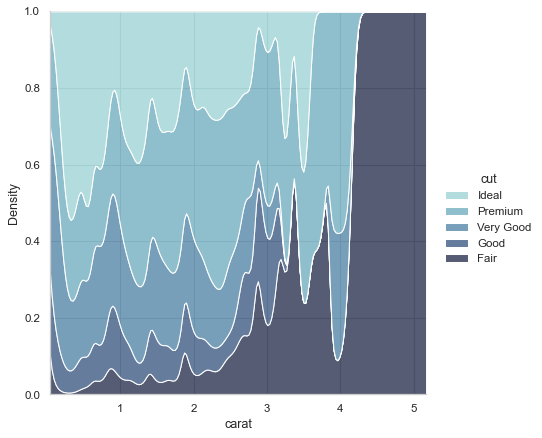
\includegraphics[width=0.37\linewidth]{kde}
%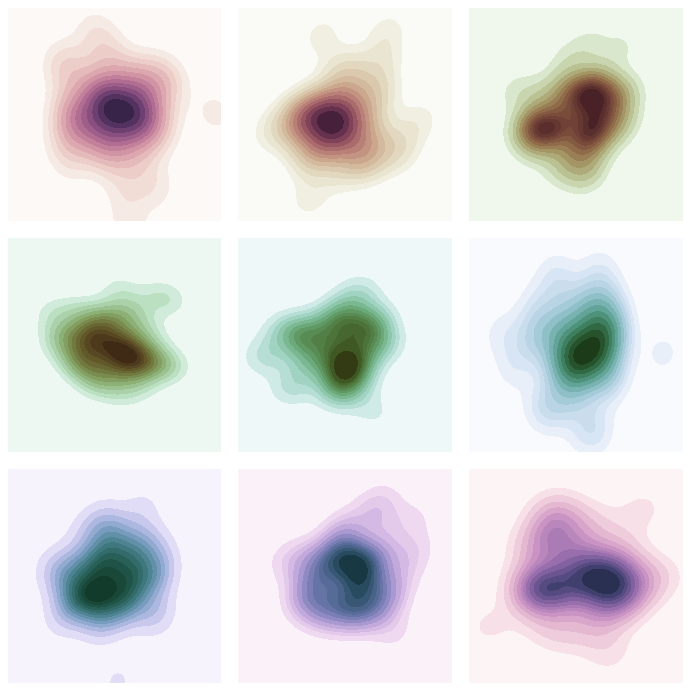
\includegraphics[width=0.3\linewidth]{palette_generation}
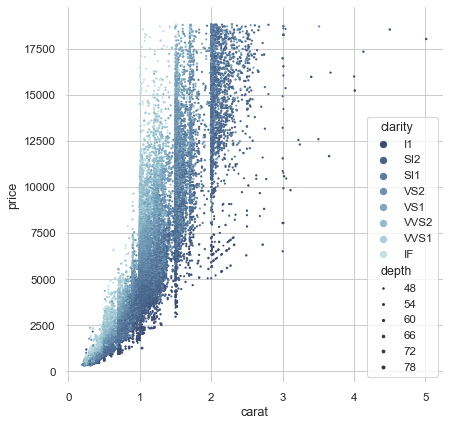
\includegraphics[width=0.32\linewidth]{scatter}

\begin{textblock*}{0.45\paperwidth}(0.65\paperwidth,0.1\paperheight)
	\footnotesize
	\textcolor{gray}{\href{https://seaborn.pydata.org/examples/}{\underline{seaborn illustrations}}}
\end{textblock*}

\end{frame}

%------------------------------------------------

\subsection{linear models}
\begin{frame}
\myframetitle{0.45\paperwidth}{0.04\paperwidth}{\insertsection}
\myframesubtitle{0.47\paperwidth}{\insertsubsection}
\centering
\vspace{0.2\paperheight}
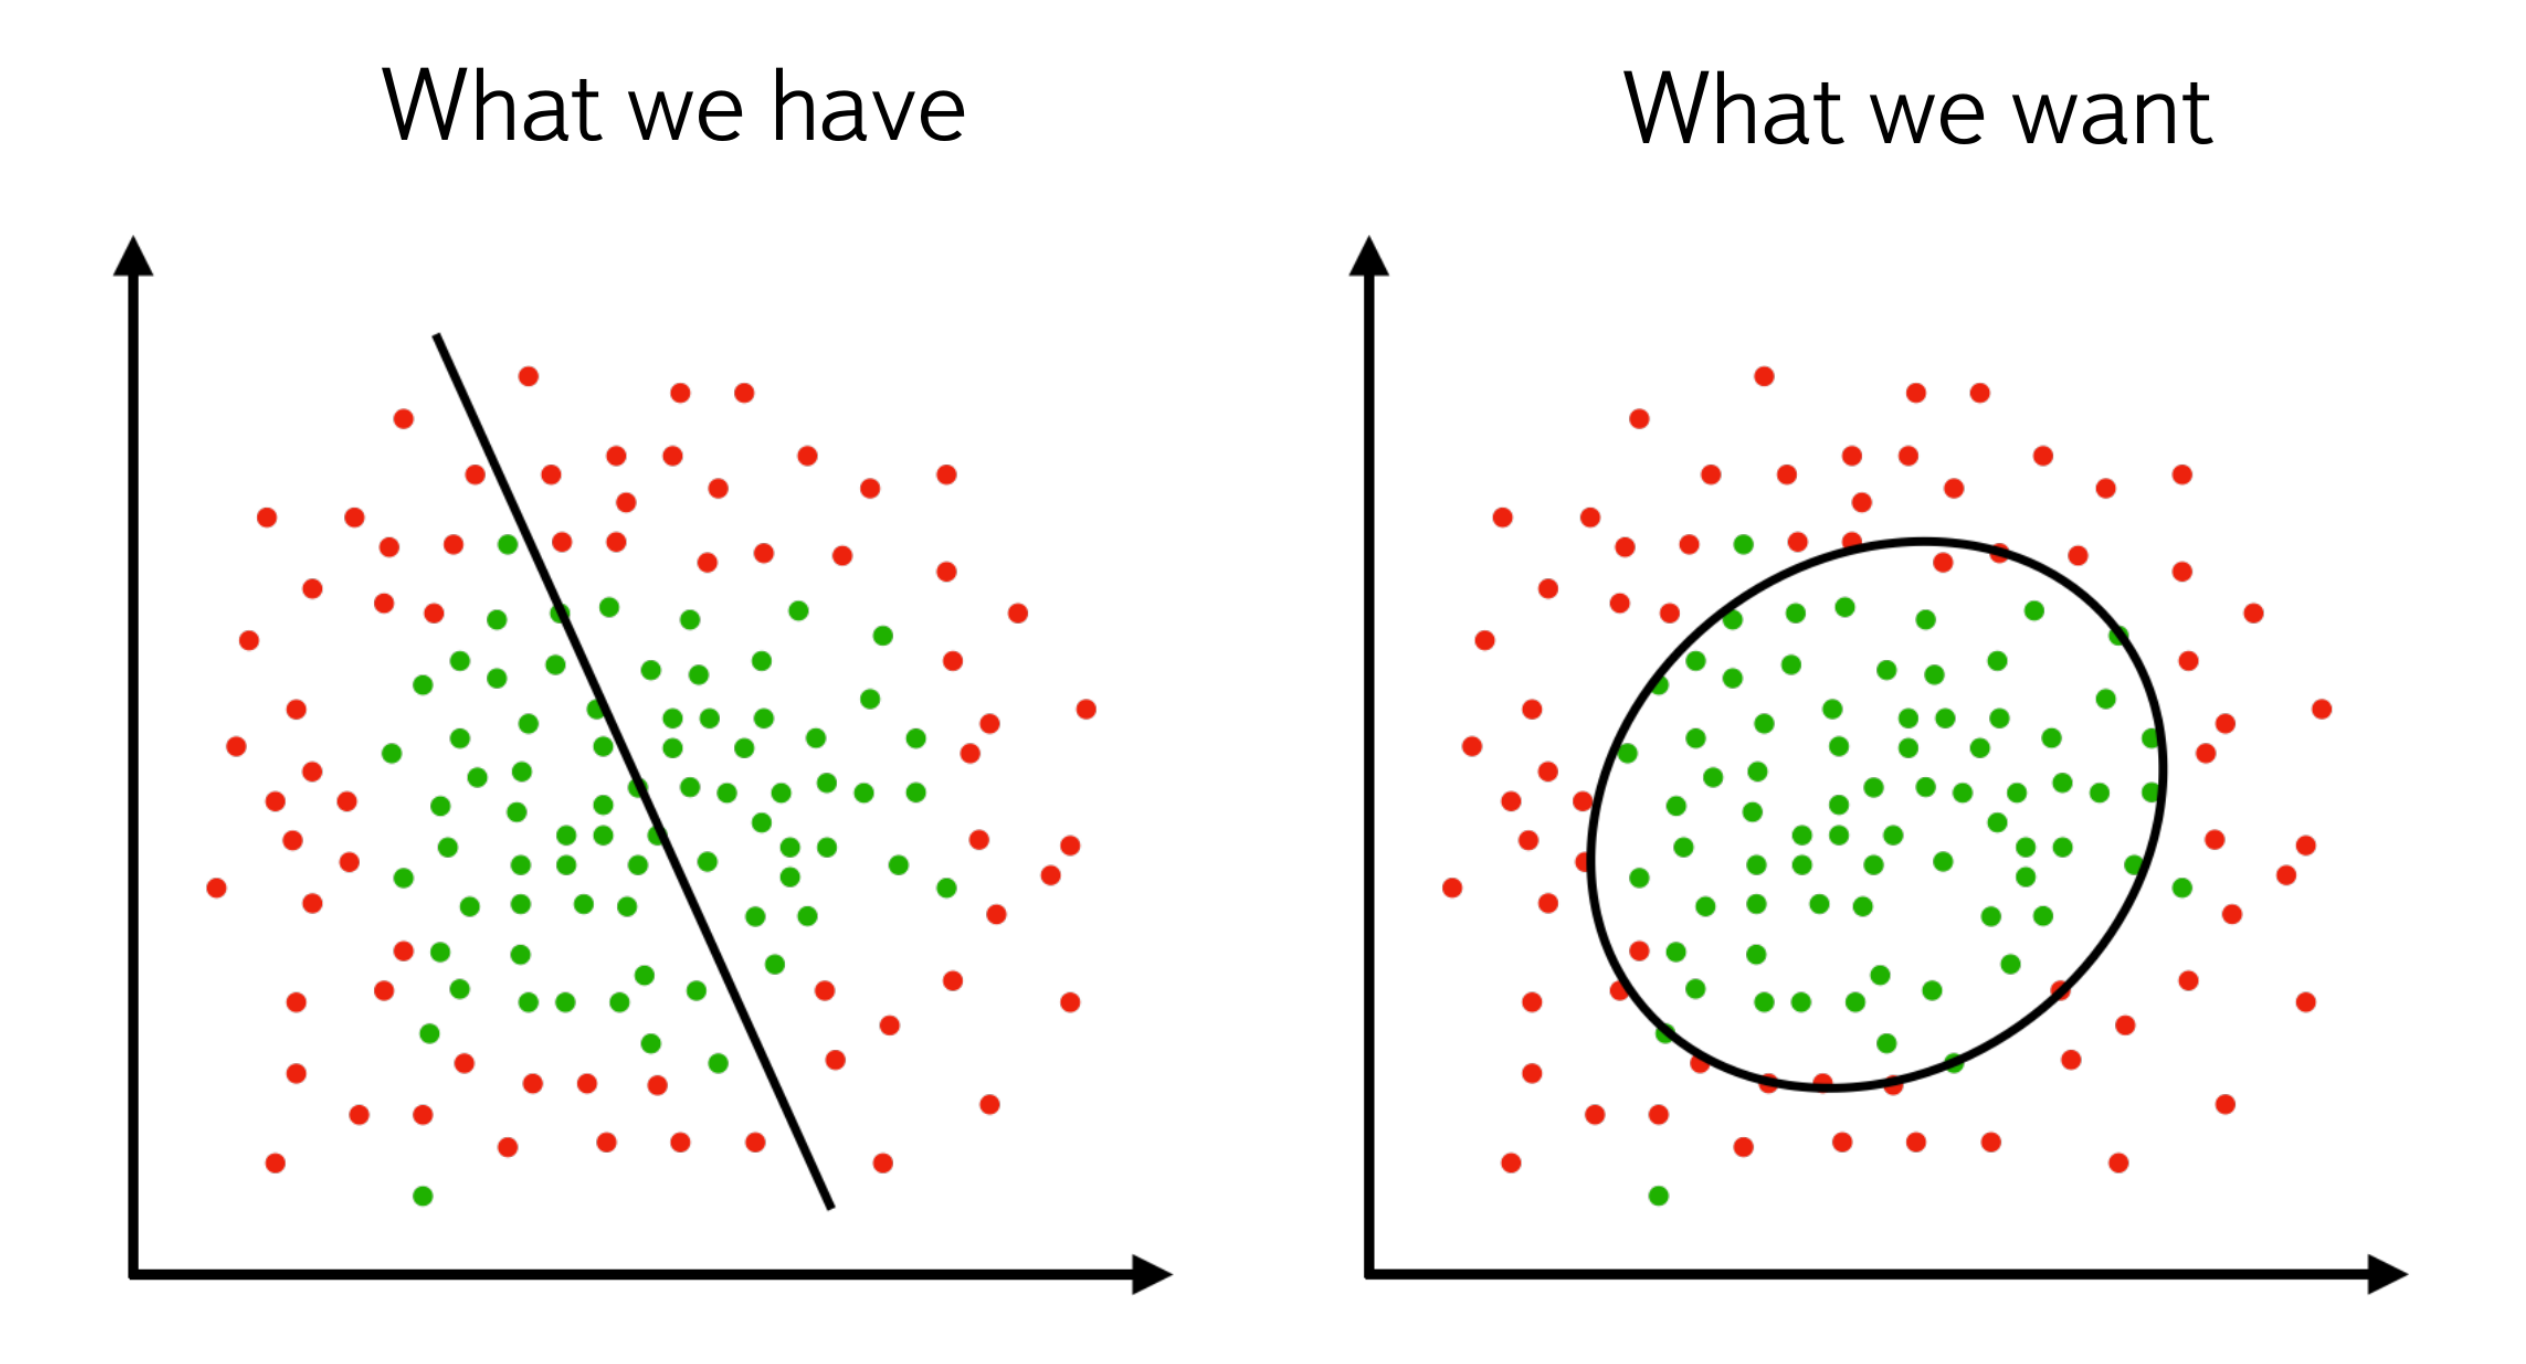
\includegraphics[width=0.6\linewidth]{images/want_have.png}\\

\centering
\footnotesize
\vspace{0.05\paperheight}
Linear models can't simply describe complex nonlinear data

\end{frame}

%------------------------------------------------

\subsection{trees}
\begin{frame}
\myframetitle{0.45\paperwidth}{0.04\paperwidth}{\insertsection}
\myframesubtitle{0.47\paperwidth}{\insertsubsection}

\vspace{0.15\paperheight}
\begin{columns}
\column{0.63\textwidth}
\begin{minipage}{\linewidth}
\begin{itemize}
	\small
	\setbeamertemplate{items}{\mybullet}
	\item (Ensembles of) Trees were designed to approximate nonlinearities and are \textbf{pretty good} in it + they are \textbf{fast and interpretable}
	\item But they are just "brute-force" algorithms -- \textbf{don't infer symmetries} in data by design
	\item \textbf{Ad-hoc, cut-based and piecewise approximations} of data at hand + not differentiable and smooth
\end{itemize}
\end{minipage}

\column{0.4\textwidth}
\begin{minipage}{\linewidth}
\centering
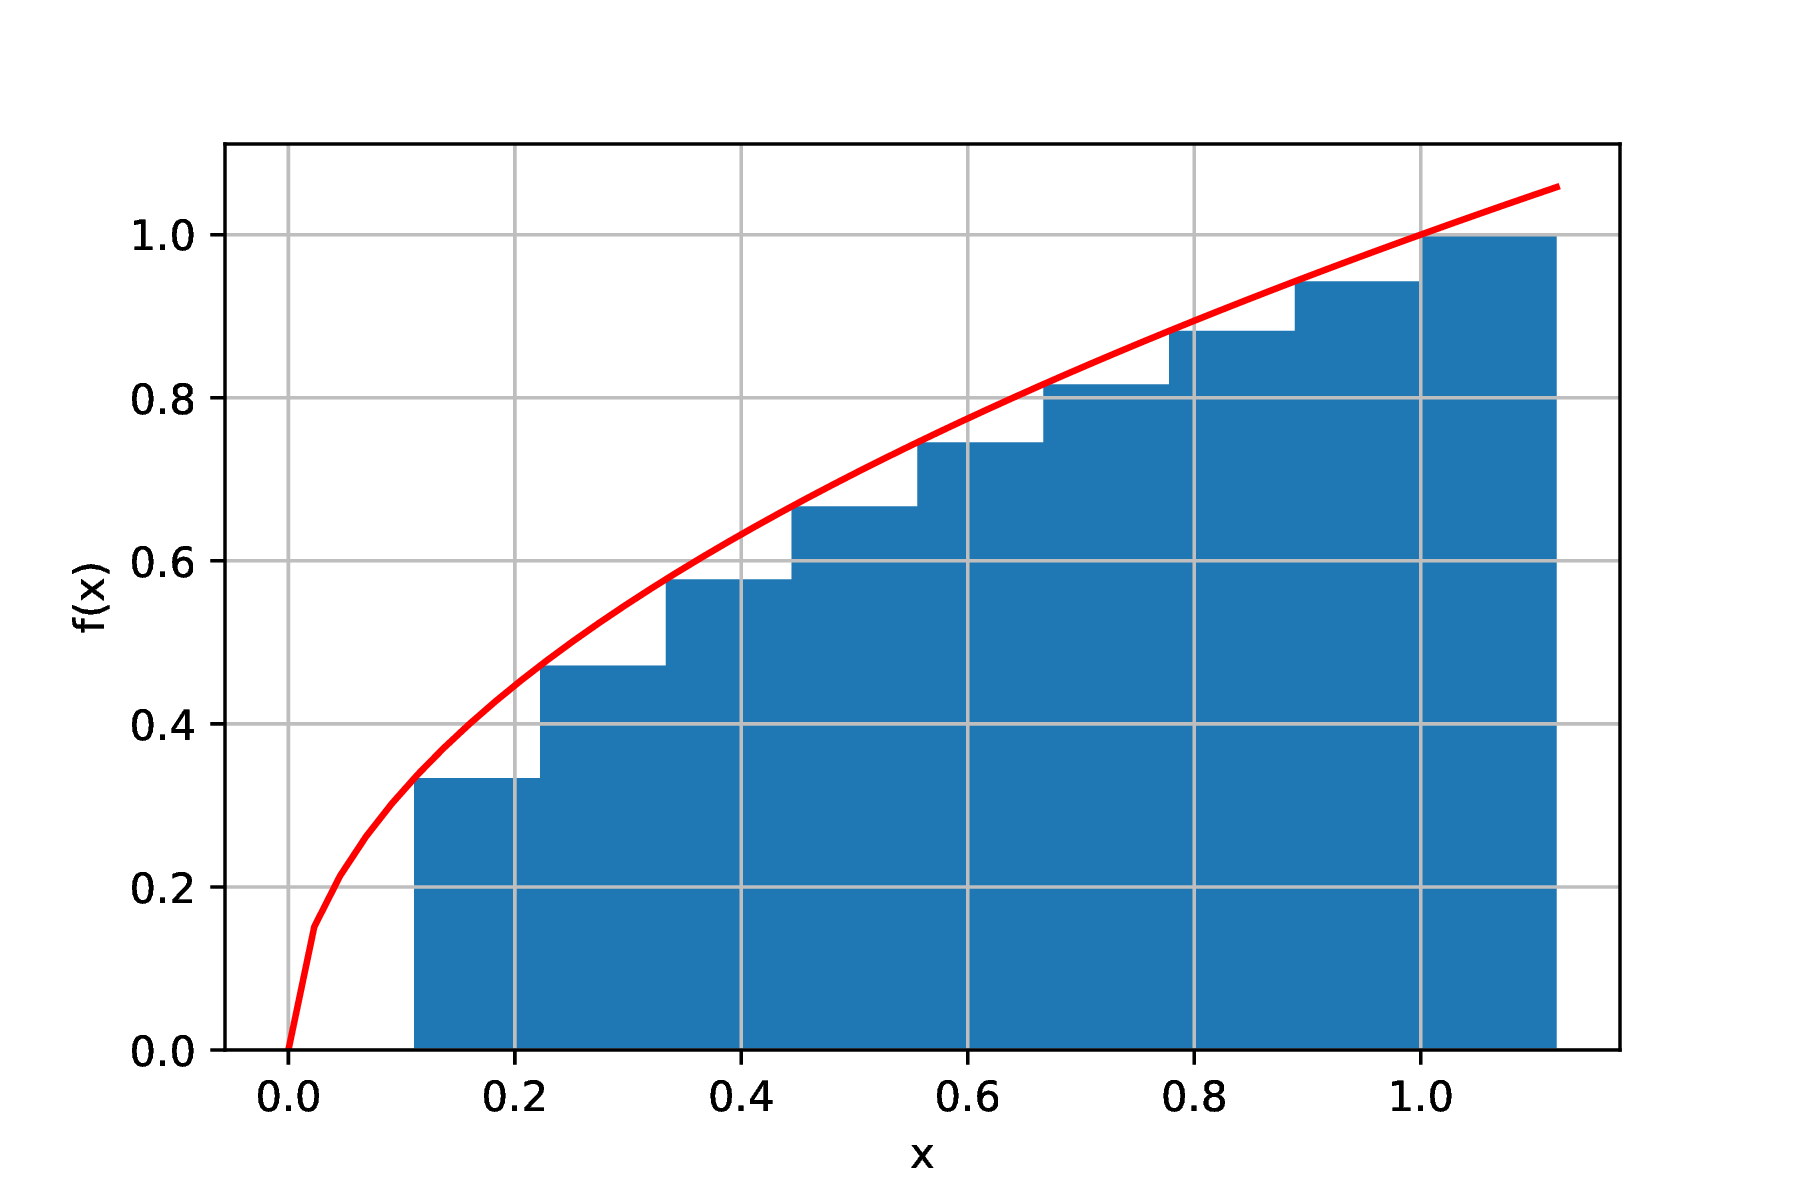
\includegraphics[width=0.8\linewidth]{images/plot.png}\\
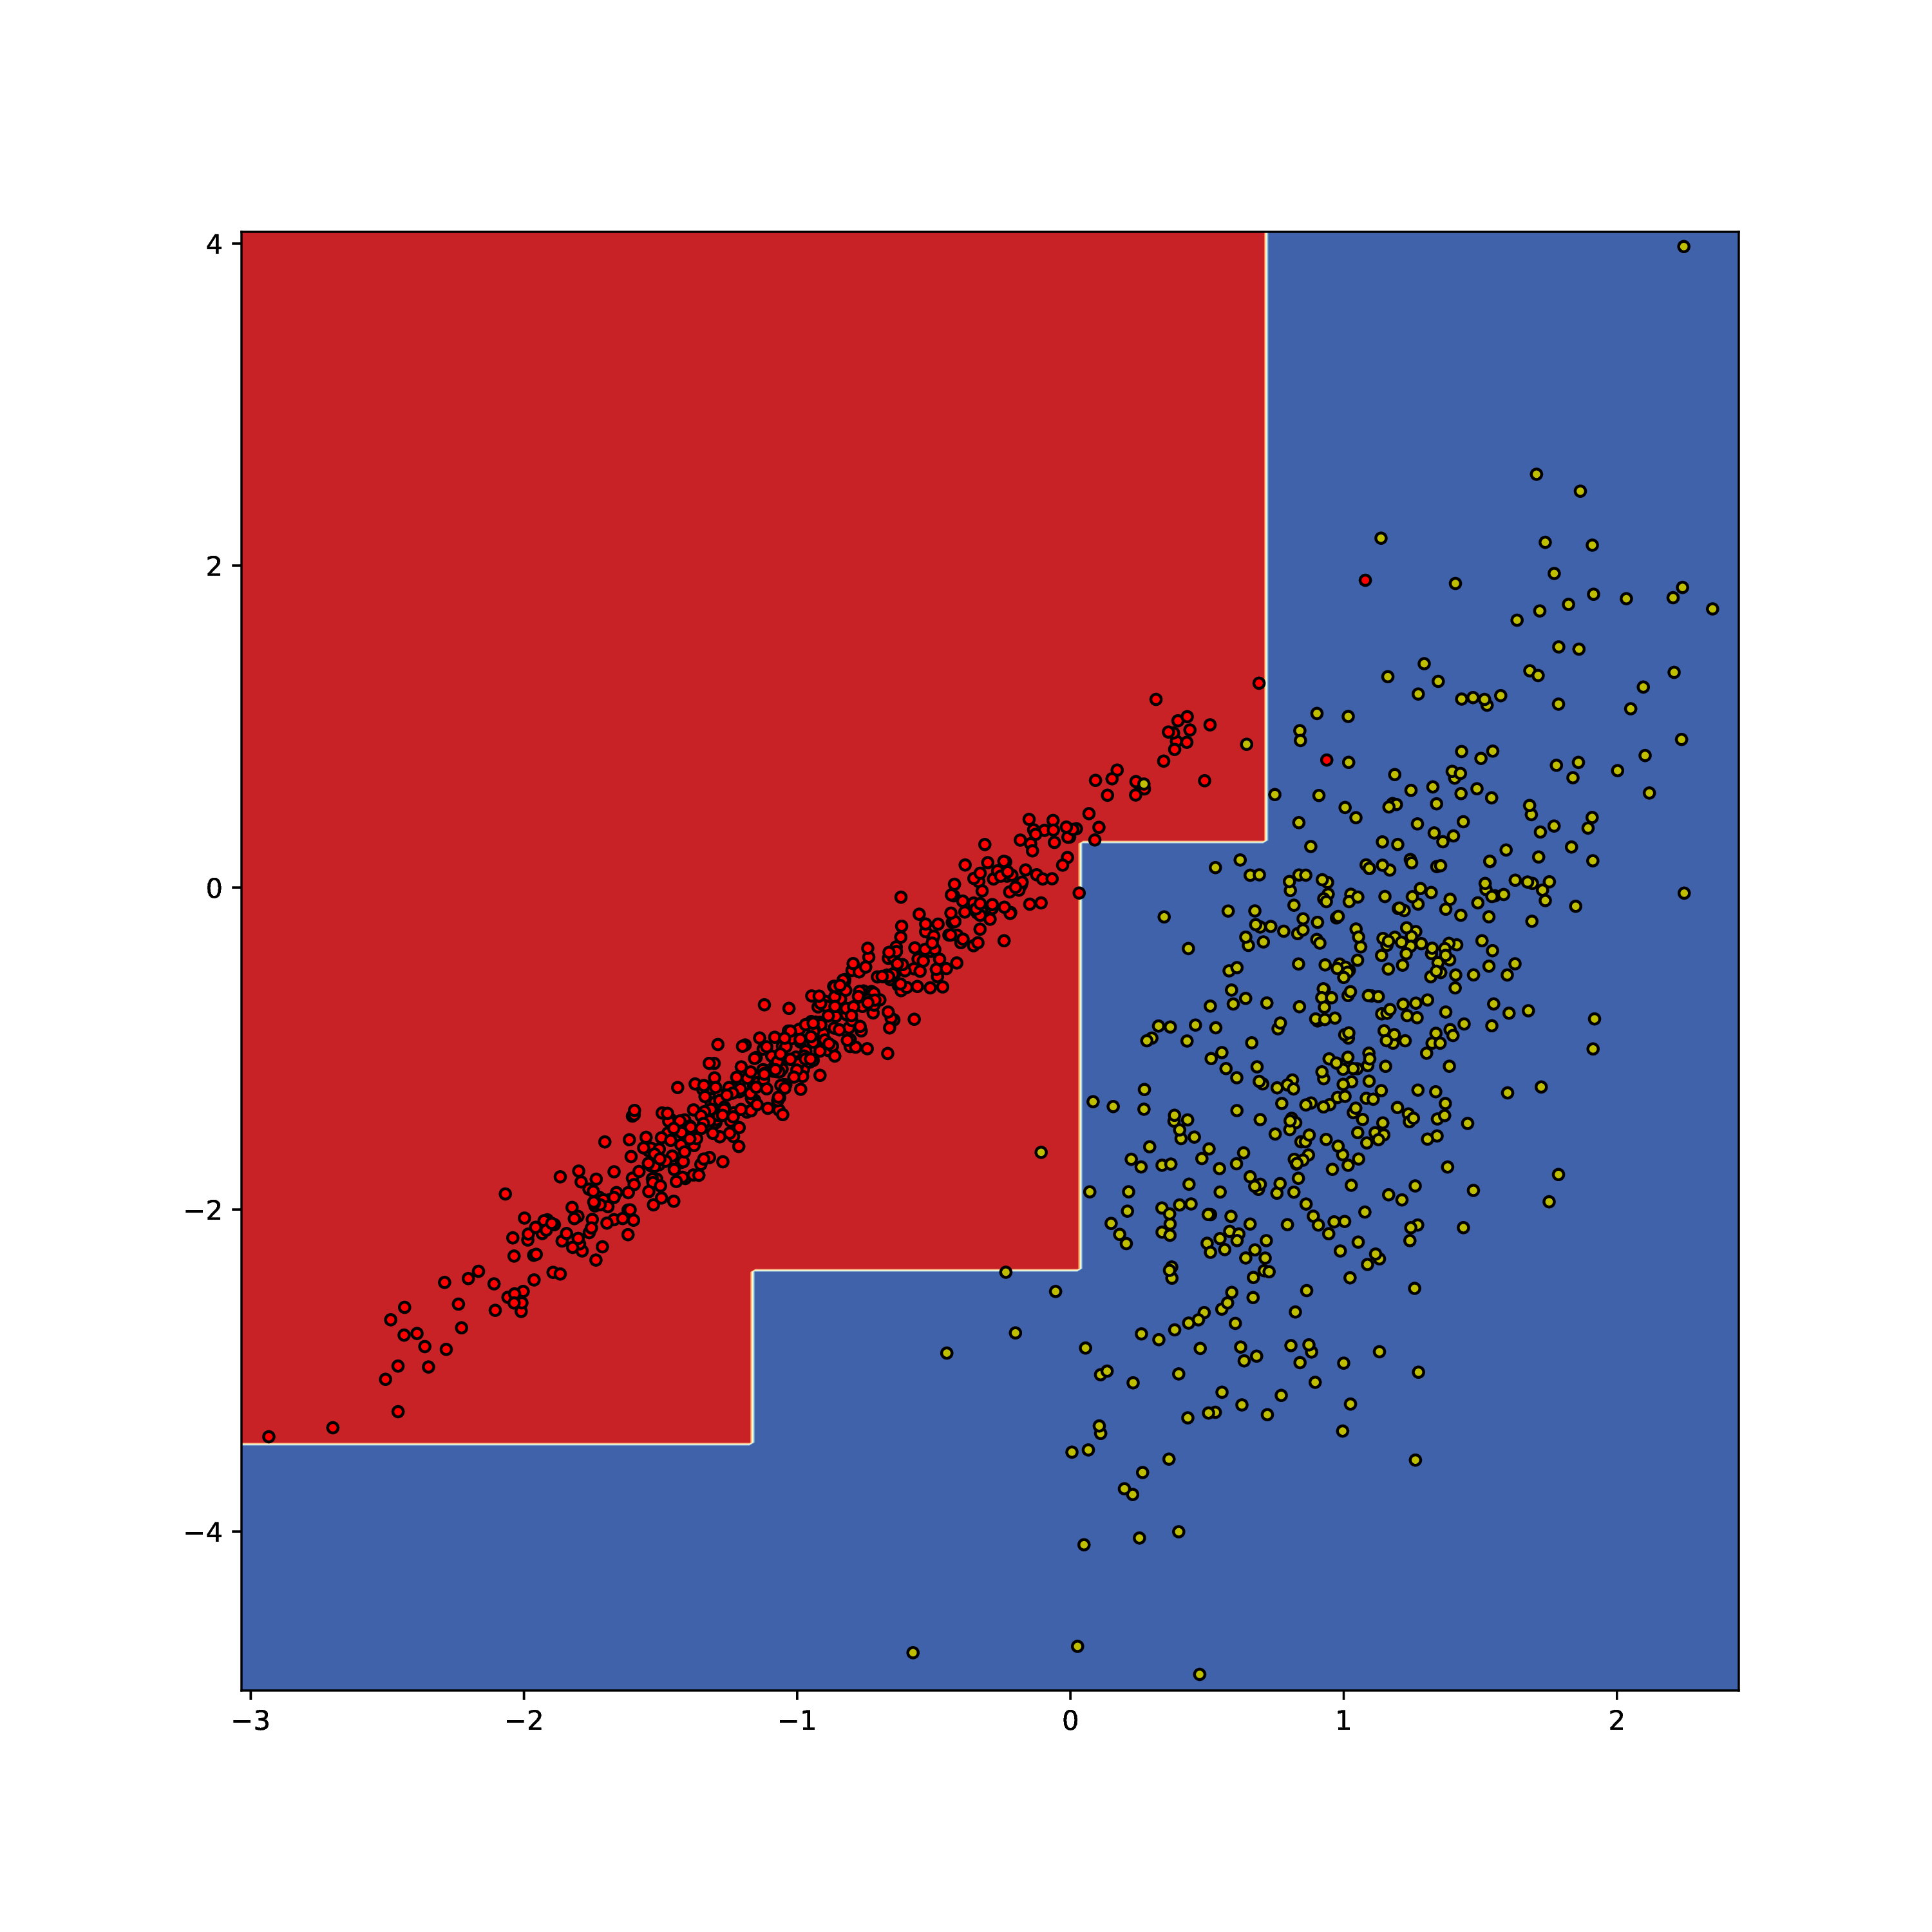
\includegraphics[width=0.8\linewidth]{images/4gi.png}\\
\end{minipage}
\end{columns}
\end{frame}

%------------------------------------------------

\subsection{feature engineering}
\begin{frame}
\myframetitle{0.45\paperwidth}{0.04\paperwidth}{\insertsection}
\myframesubtitle{0.47\paperwidth}{\insertsubsection}
\centering
\vspace{1.7cm}
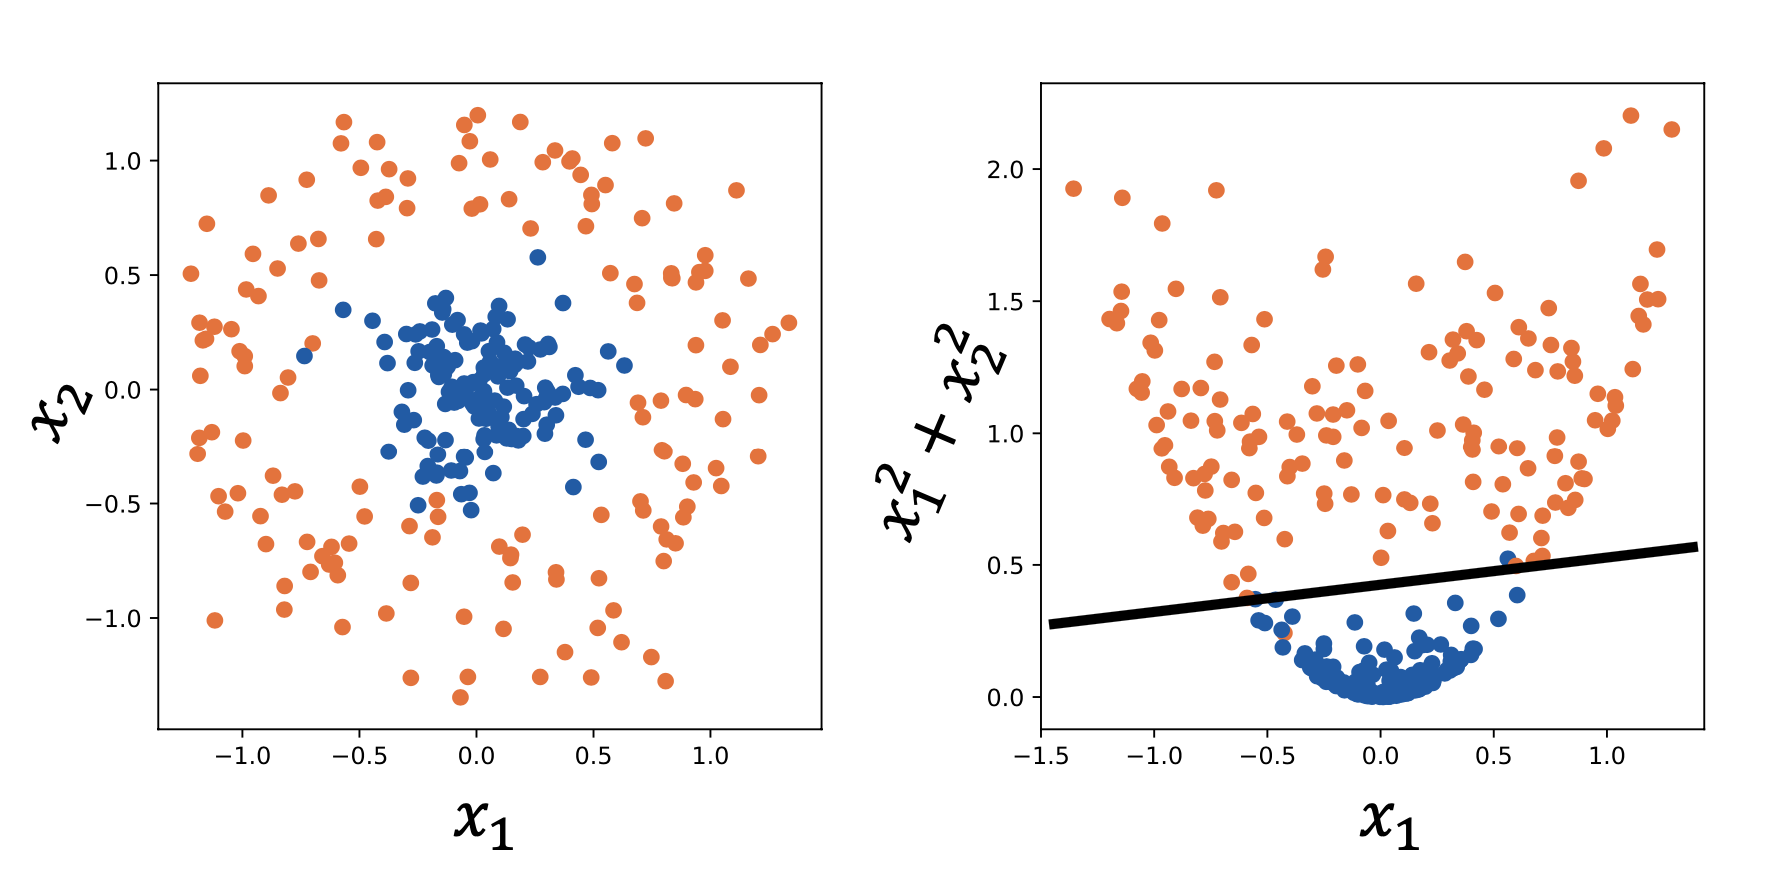
\includegraphics[width=0.5\linewidth]{images/feature_engin.png}\\
\begin{itemize}
	\small
	\setbeamertemplate{items}{\mybullet}
	\item But sometimes we know \textit{a priori} that there are transformations simplifying the problem $\rightarrow$ even linear model can do the job
	\item However, this \textbf{feature engineering} is non-trivial, requires domain knowledge and is time-consuming
\end{itemize}

\only<2->{
\begin{textblock*}{0.9\textwidth}(0.1\paperwidth, 0.89\paperheight)
	\centering
	\small
	\textcolor{myorange}{What if we design a model which could \textbf{automatically} feature-engineer itself?}
\end{textblock*}

}
\end{frame}

%------------------------------------------------
%------------------------------------------------
\section{Neural Network}
%------------------------------------------------
%------------------------------------------------

\begin{frame}[plain]
\centering
\huge
%\begin{textblock*}{0.3\paperwidth}(0.25\paperwidth,0.3\paperheight)
\centering
\vspace{0.1\paperheight}
\begin{tcolorbox}[colframe=white, colback=mygrey, width=0.5\paperwidth,
arc=2.mm, boxsep=2mm,
box align=center,
halign=center,
valign=center,
]
\insertsection
\end{tcolorbox}
%\end{textblock*}
\transfade[duration=.4]
\end{frame}

%------------------------------------------------

\subsection{automating FE}
\begin{frame}
\myframetitle{0.35\paperwidth}{0.04\paperwidth}{\insertsection}
\myframesubtitle{0.35\paperwidth}{\insertsubsection}
\centering

\vspace{0.6\paperheight}
\begin{textblock*}{0.5\paperwidth}(0.27\paperwidth, 0.25\paperheight)
	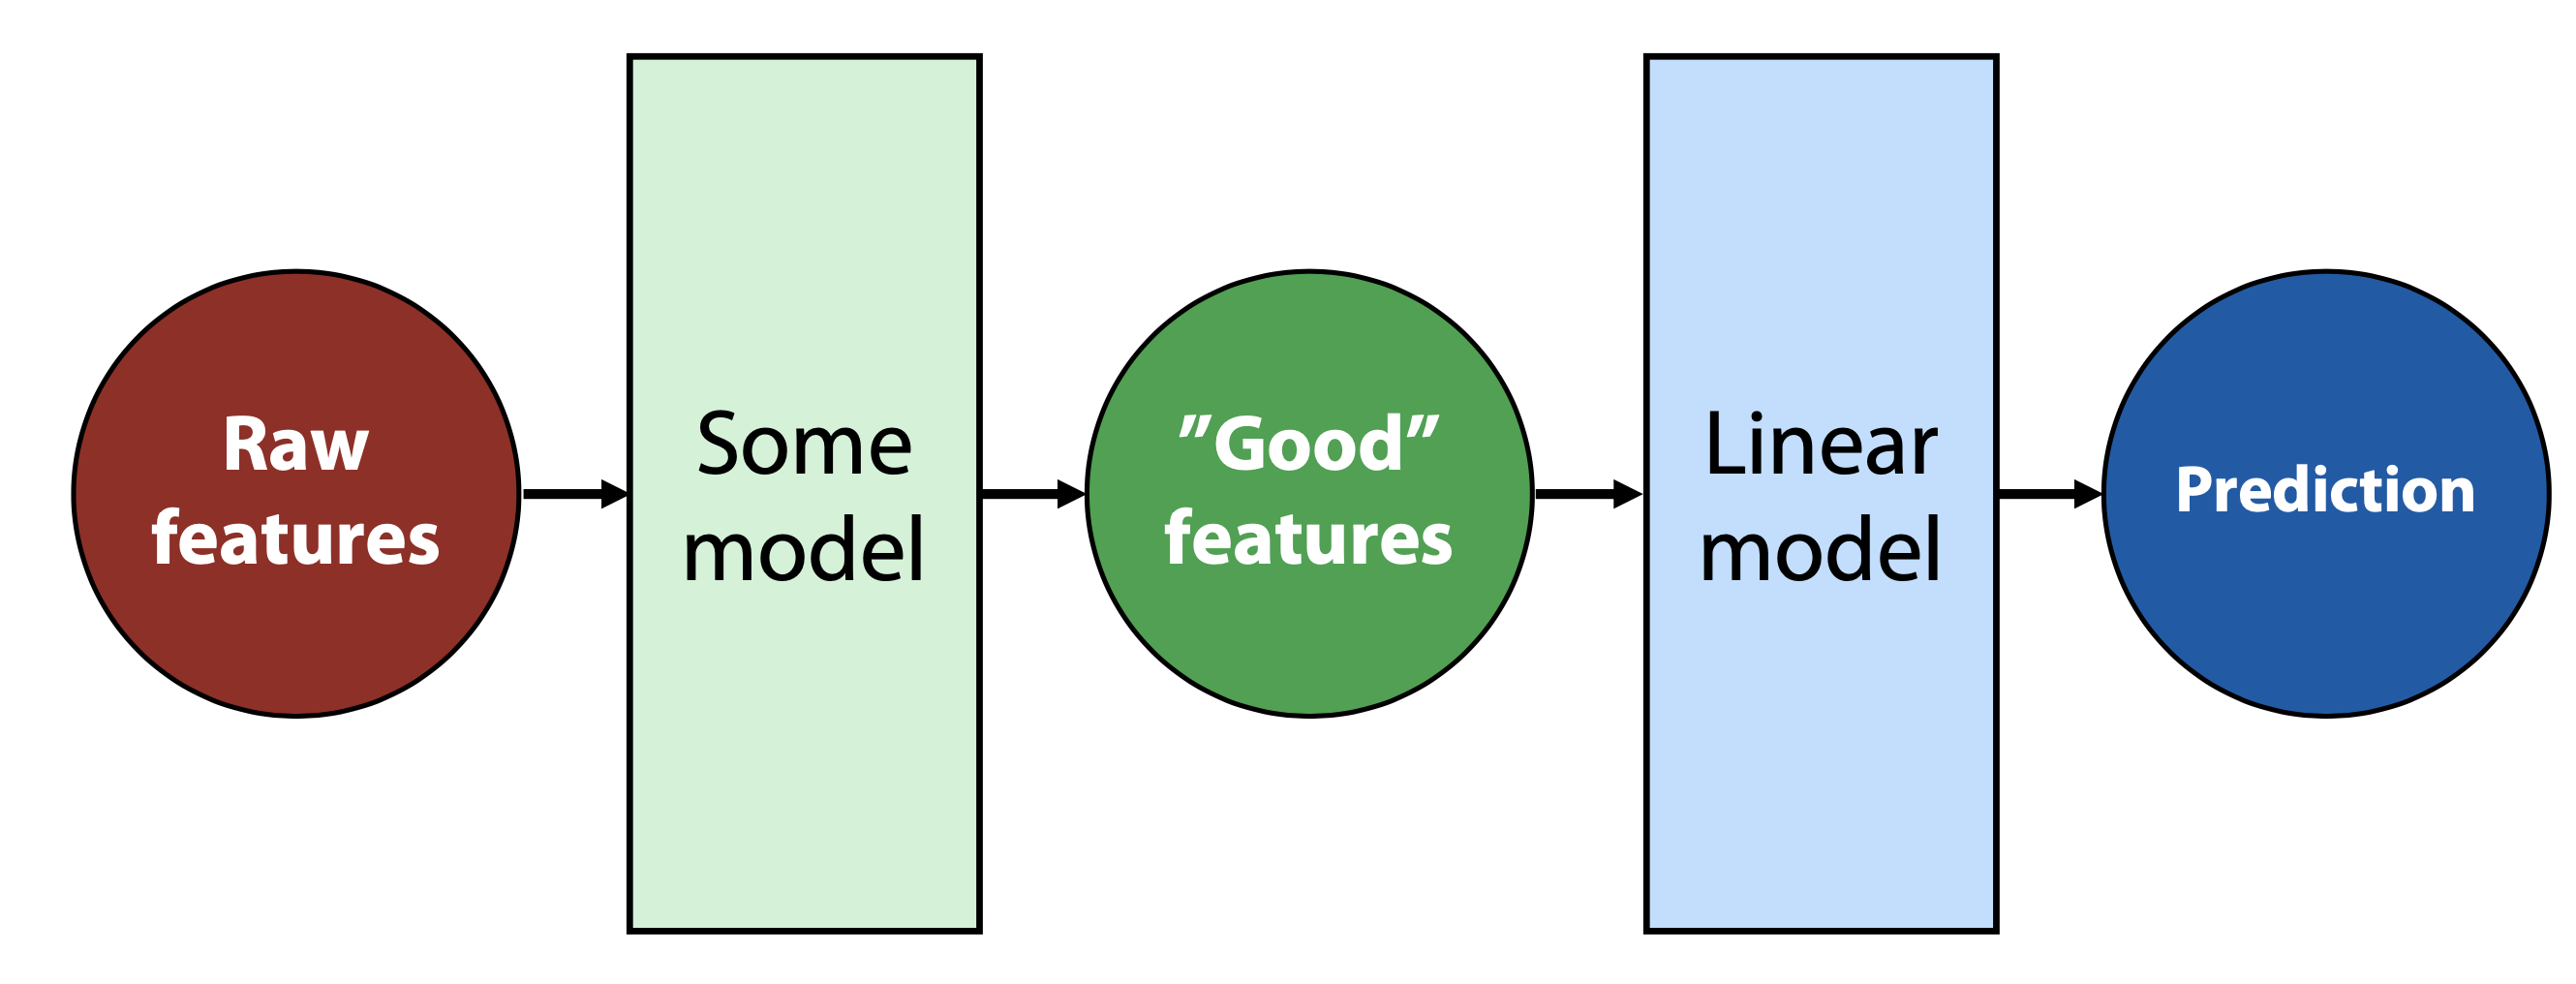
\includegraphics[width=1.\linewidth]{images/some_model.png}
\end{textblock*}

\vspace{0.02\paperheight}
\begin{itemize}
	\footnotesize
	\setbeamertemplate{items}{\mybullet}
	\item Let's use a \textbf{simple linear model} to solve our supervised problem 
	\item Add a block to a linear model which will automatically \textbf{generate new features} for it 
	\item Two blocks would work together as a \textbf{single model} $\Rightarrow$ their parameters are updated simultaneously
	\item And \textbf{automatically}, by e.g. gradient descent (given their differentiability)
\end{itemize}

\begin{textblock*}{0.25\paperwidth}(0.75\paperwidth,0.1\paperheight)
	\scriptsize
	\textcolor{gray}{NN illustrations from \href{https://indico.cern.ch/event/838377/}{\underline{ML in HEP 2020}}}
\end{textblock*}

\end{frame}

%------------------------------------------------

\begin{frame}
\myframetitle{0.35\paperwidth}{0.04\paperwidth}{\insertsection}
\myframesubtitle{0.35\paperwidth}{\insertsubsection}

\vspace{0.6\paperheight}
\begin{textblock*}{0.5\paperwidth}(0.27\paperwidth, 0.25\paperheight)
	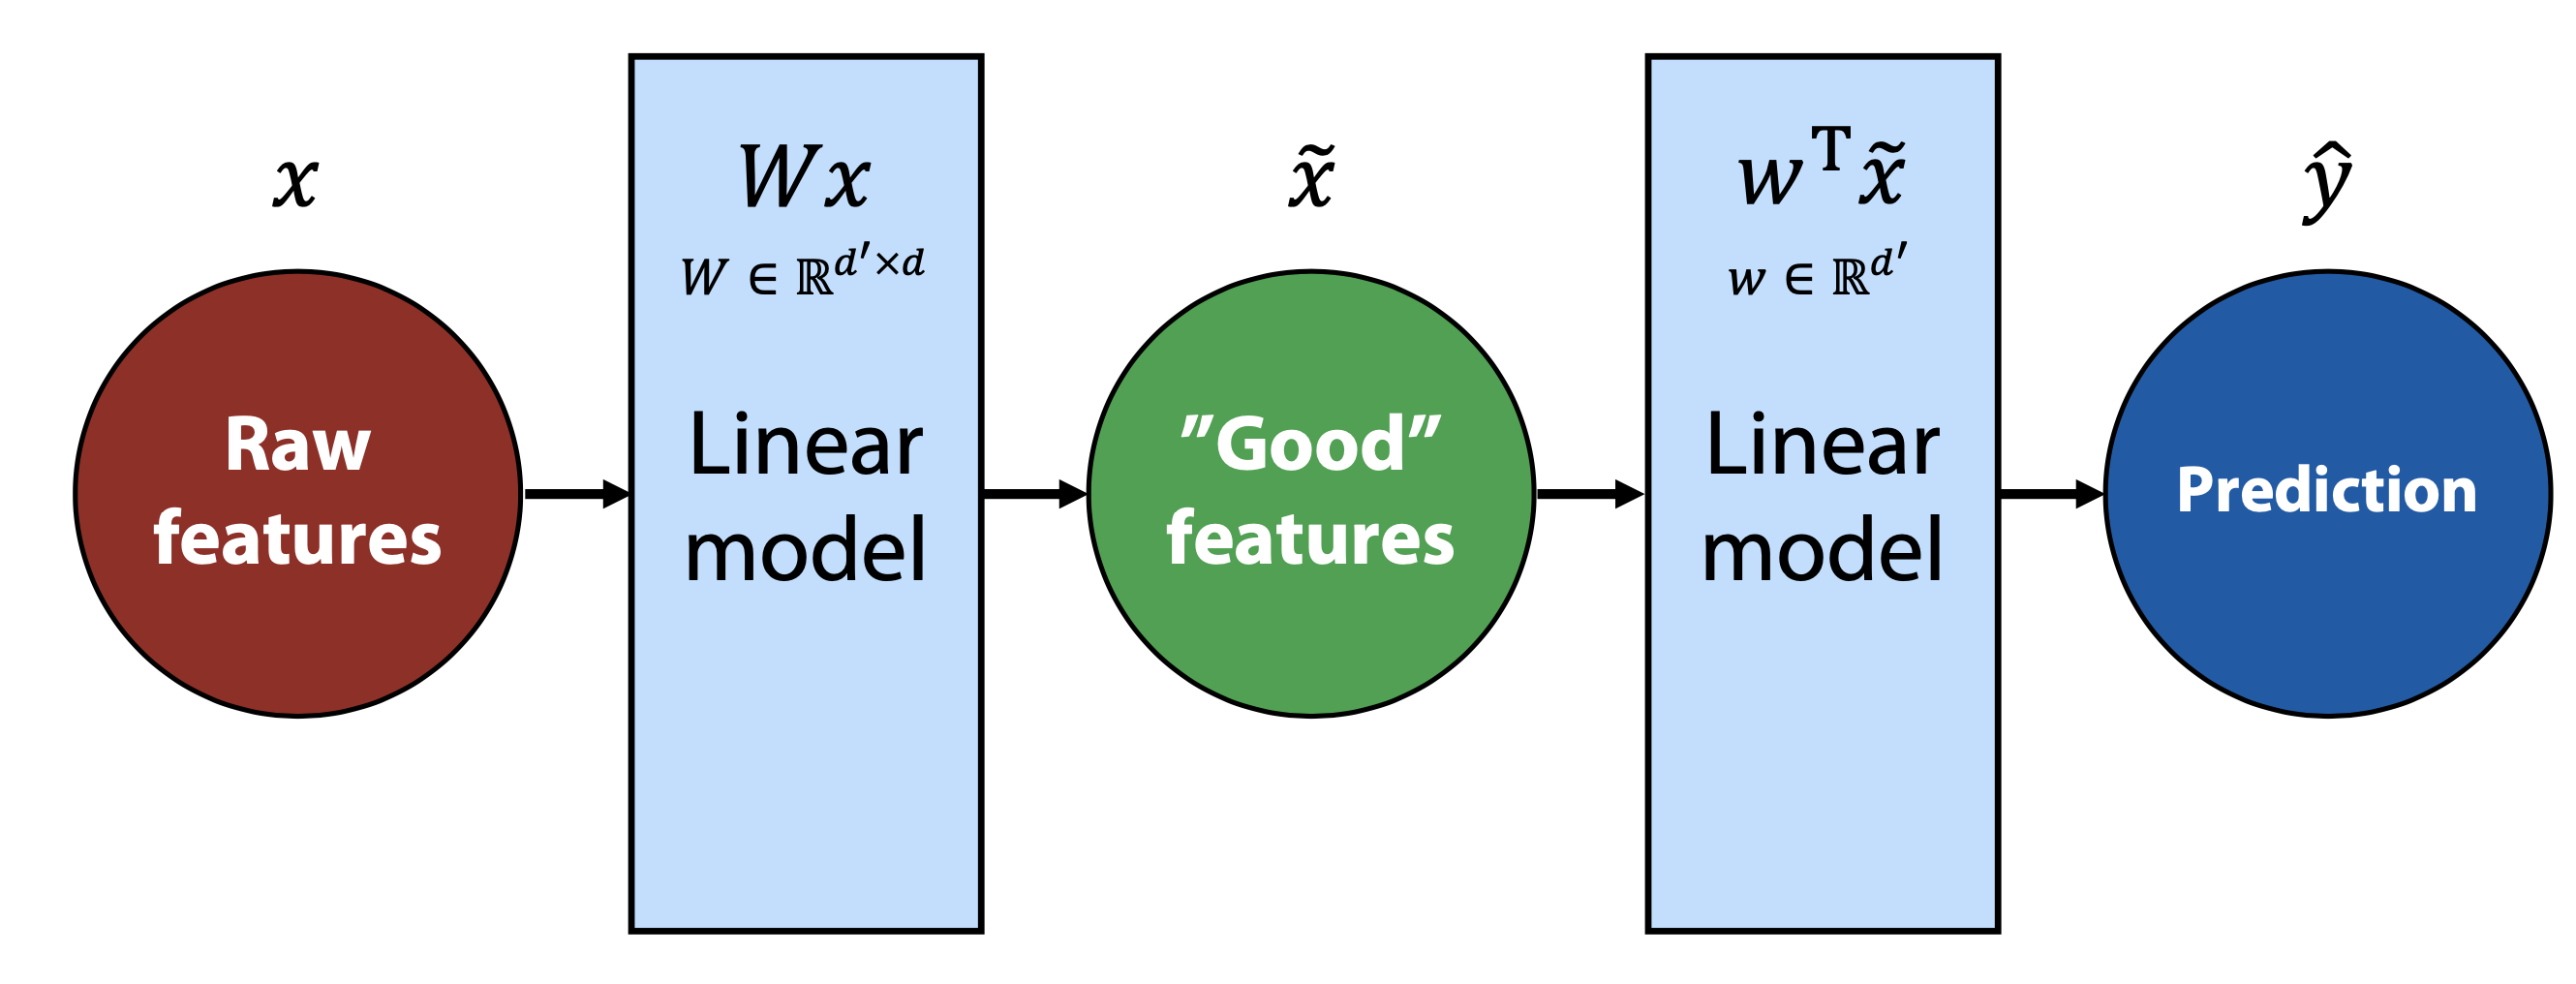
\includegraphics[width=1.\linewidth]{images/lin_model.png}
\end{textblock*}

\begin{itemize}
	\footnotesize
	\setbeamertemplate{items}{\mybullet}
	\item Would a linear model work as a feature generating model? \only<2->{\textcolor{myorange}{No}}
	\item<2> {$\hat{y} = w^{T}\tilde{x} = w^{T} (W x) = (w^{T} W) x = w'^{T} x \Rightarrow$ it is still a linear model}
	\item<2>[\textcolor{myorange}{\MVRightArrow}] \textcolor{myorange}{Input feature space has not changed, only the model weights}
\end{itemize}
\end{frame}

%------------------------------------------------

\begin{frame}
\myframetitle{0.35\paperwidth}{0.04\paperwidth}{\insertsection}
\myframesubtitle{0.35\paperwidth}{\insertsubsection}

\vspace{0.6\paperheight}
\begin{textblock*}{0.5\paperwidth}(0.27\paperwidth, 0.25\paperheight)
	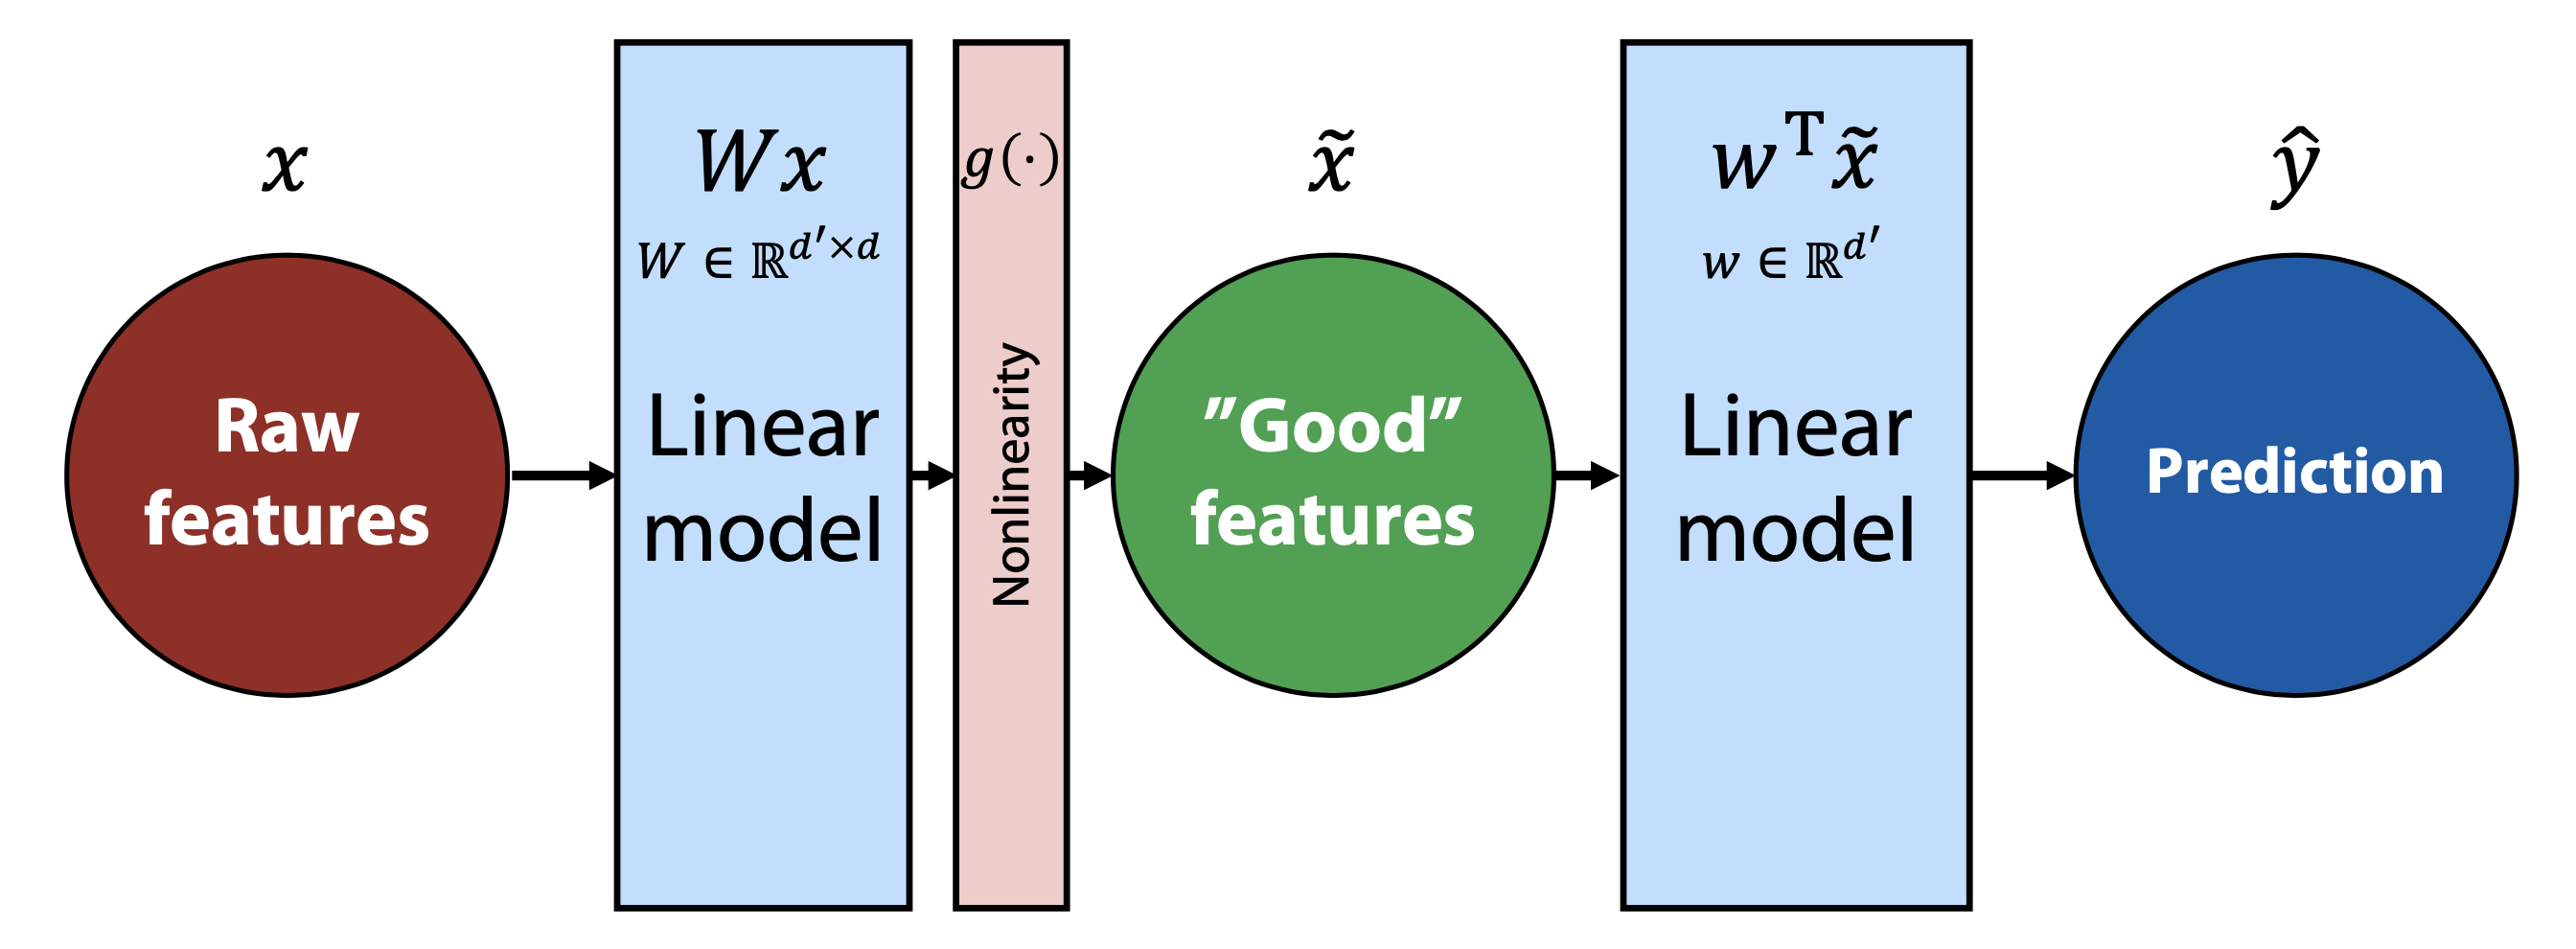
\includegraphics[width=1.\linewidth]{images/add_nonlin.png}
\end{textblock*}

\begin{itemize}
	\footnotesize
	\setbeamertemplate{items}{\mybullet}
	\item Let's then introduce \textbf{nonlinearity} to our model
	\item[\textcolor{myblack}{\MVRightArrow}] $\hat{y} = w^{T} \tilde{x} = w^{T} g(W x)$,\\
where $g(\cdot)$ -- some nonlinear scalar function (applied elementwise)
	\item<2->[\textcolor{myblack}{\MVRightArrow}] This is the simplest example of a \textcolor{myorange}{\textbf{neural network}}
\end{itemize}
\end{frame}

%------------------------------------------------

%\begin{frame}[plain]
%\centering
%\huge
%
%%\begin{textblock*}{0.3\paperwidth}(0.25\paperwidth,0.3\paperheight)
%\centering
%\vspace{0.1\paperheight}
%\begin{tcolorbox}[colframe=white, colback=mygrey, width=0.4\paperwidth,
%	arc=2.mm, boxsep=2mm,
%	box align=center,
%	halign=center,
%	valign=center,
%	]
%	\insertsection
%\end{tcolorbox}
%
%%\end{textblock*}
%
%\transfade[duration=.4]
%\end{frame}

%------------------------------------------------

\subsection{architecture}
\begin{frame}
\myframetitle{0.35\paperwidth}{0.04\paperwidth}{\insertsection}
\myframesubtitle{0.35\paperwidth}{\insertsubsection}

\vspace{0.68\paperheight}
\begin{textblock*}{0.65\paperwidth}(0.21\paperwidth, 0.25\paperheight)
	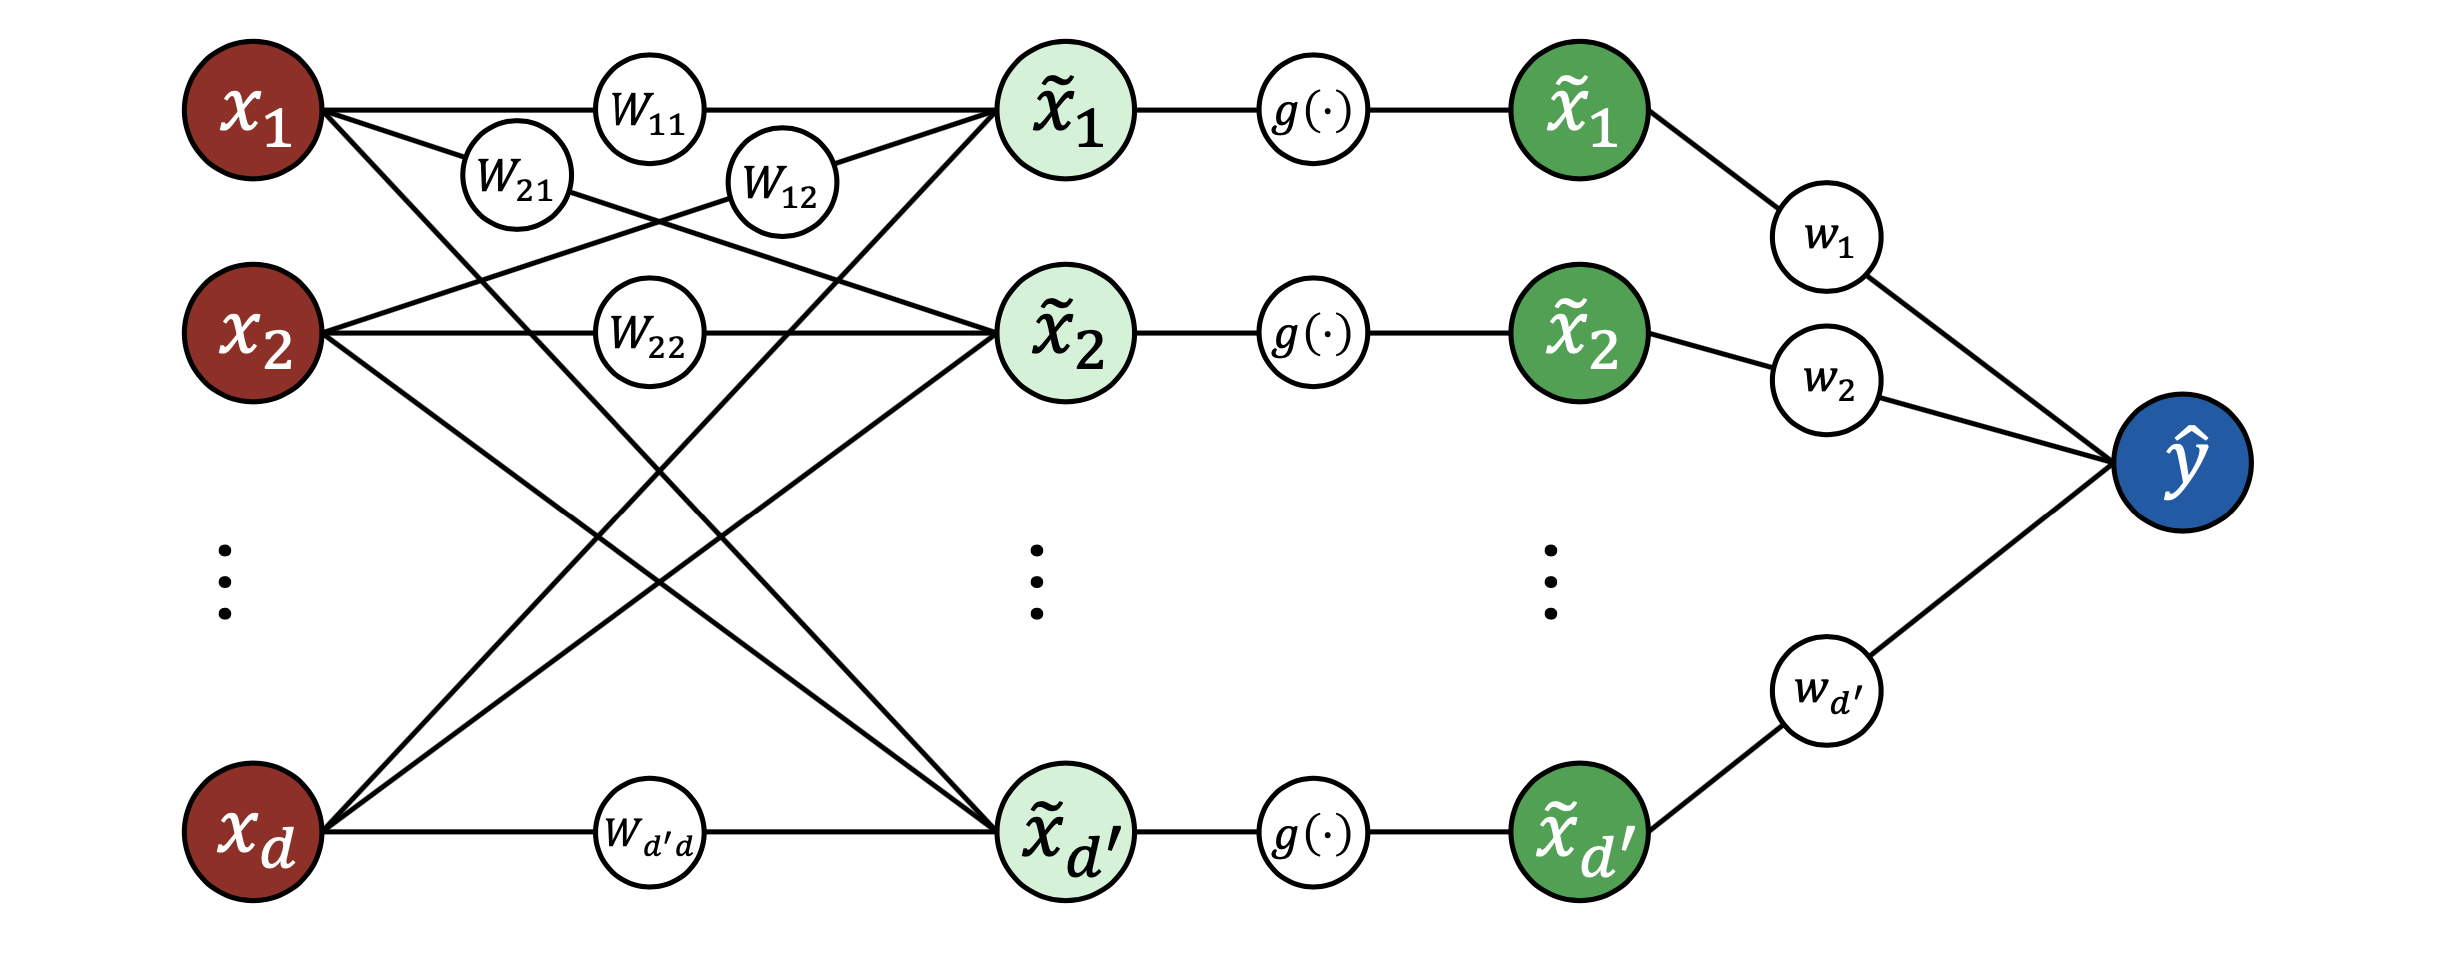
\includegraphics[width=1.\linewidth]{images/nn_details.png}
\end{textblock*}

\begin{itemize}
\centering
\small
\setbeamertemplate{items}{\mybullet}
\item[] Essentially, NN is just a \textbf{composite function} that maps a set of $X$ to a set of $Y$
\item[] $\hat{y} = w^{T} \tilde{x} = w^{T} g(W x)$
\end{itemize}
\end{frame}

%------------------------------------------------

\subsection{terminology}
\begin{frame}
\myframetitle{0.35\paperwidth}{0.04\paperwidth}{\insertsection}
\myframesubtitle{0.35\paperwidth}{\insertsubsection}
\centering
\vspace{2.cm}

\begin{columns}
	
\column{0.4\textwidth}
\begin{minipage}{\linewidth}
\begin{center}
\textbf{Feed-forward network:}\\
\hfill \break
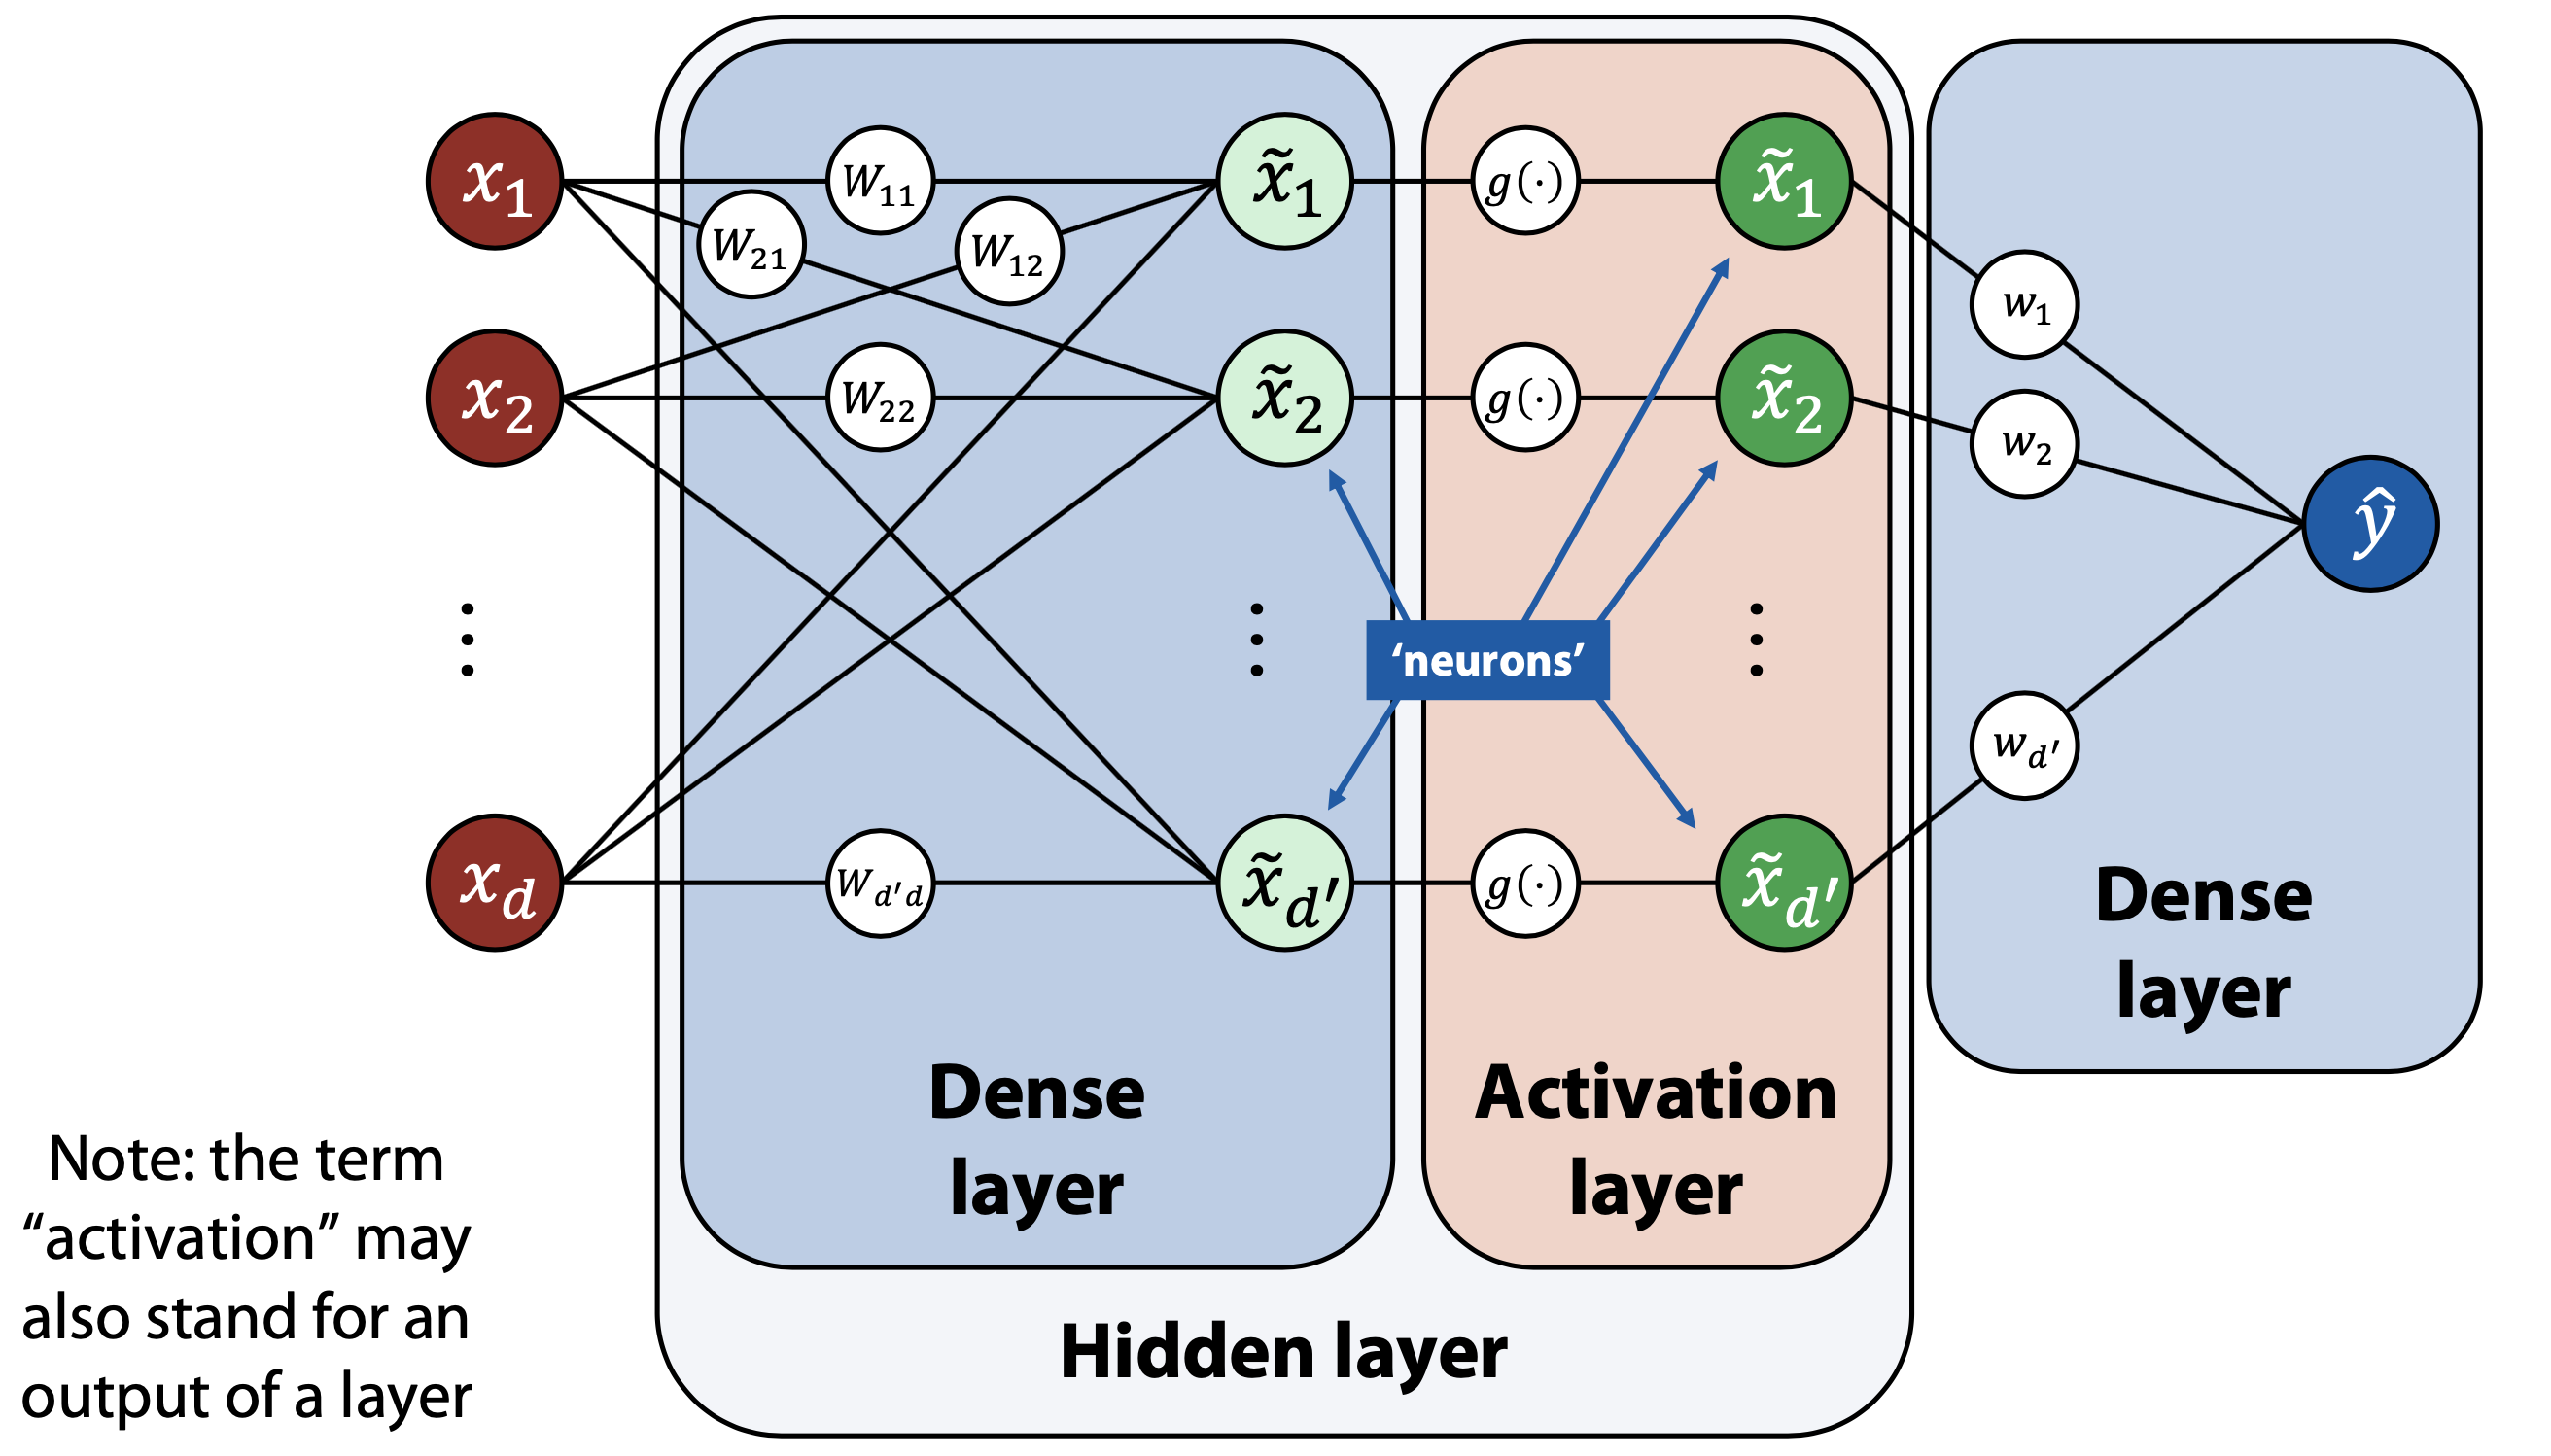
\includegraphics[width=1.0\linewidth]{images/nn_terminology.png}
\end{center}
\end{minipage}

\column{0.7\textwidth}
\begin{minipage}{\linewidth}
\begin{itemize}
	\small
	\itemsep1.ex
	\setbeamertemplate{items}{\mybullet}
	\item {\textcolor{Brown}{Brown} nodes $x_{1}, x_{2}, ..., x_{d}$ -- features from an \textbf{input layer}}
	\item {\textcolor{mygreen}{Green} nodes $\tilde{x}_{1}, \tilde{x}_{2}, ..., \tilde{x}_{d\prime}$-- \textbf{neurons} from a \textbf{hidden layer}}
	\item {\textcolor{MidnightBlue}{Blue} node $\hat{y}$ -- neuron from an \textbf{output layer}}
	\item {Straight lines (edges) between neurons -- \textbf{weights} $w_{ij}$}
	\item {$g(\cdot)$ -- nonlinear \textbf{activation} function, e.g. sigmoid $\sigma(\cdot)$}
	\item {\textcolor{myorange}{Important:} each neuron has additional \textbf{bias} $b$ associated to it and added to other inputs (not illustrated)}
\end{itemize}
\end{minipage}
\end{columns}

\end{frame}

%------------------------------------------------

\subsection{human brain}
\begin{frame}
\myframetitle{0.35\paperwidth}{0.04\paperwidth}{\insertsection}
\myframesubtitle{0.35\paperwidth}{\insertsubsection}

\centering
\vspace{0.25\paperheight}
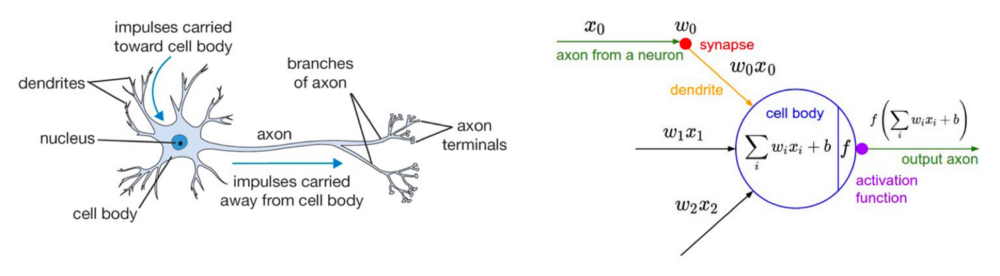
\includegraphics[width=.9\linewidth]{brain.png}
\vspace{0.07\paperheight}
\centering
\small
%Furthermore, one can think of NN as of something resembling neurons in human brain
%Neurons on human brain consist of a nucleus, dendrites, cell body, and axon. The number of neurons in humans is approximately 140 billion, consist of 100 billion neurons and 40 billion synapses in neurons.
\end{frame}

%------------------------------------------------
%------------------------------------------------
\section{Training}
%------------------------------------------------
%------------------------------------------------

\begin{frame}[plain]
\centering
\huge
%\begin{textblock*}{0.3\paperwidth}(0.25\paperwidth,0.3\paperheight)
\centering
\vspace{0.1\paperheight}
\begin{tcolorbox}[colframe=white, colback=mygrey, width=0.3\paperwidth,
arc=2.mm, boxsep=2mm,
box align=center,
halign=center,
valign=center,
]
\insertsection
\end{tcolorbox}
%\end{textblock*}
\transfade[duration=.4]
\end{frame}

%------------------------------------------------

\subsection{how to train?}
\begin{frame}
\myframetitle{0.22\paperwidth}{0.04\paperwidth}{\insertsection}
\myframesubtitle{0.23\paperwidth}{\insertsubsection}
\vspace{0.2\paperheight}

\begin{itemize}
	\small
\setbeamertemplate{items}{\mybullet}
\item Since NN fundamentally is a parametrized differentiable model we can optimise the loss function and use \textbf{gradient descent} to train it:
\[
\bm\omega_{k+1} \leftarrow \bm\omega_{k} - \eta \cdot \textcolor{mypurple}{\nabla Q (\bm\omega_{k})}
\]
\item But \textcolor{mypurple}{gradients} are hard to derive analytically -- writing down all the derivatives is tough and tedious (especially for large NN) 
\item Note that NN is just a \textbf{composite model} $\Rightarrow$ can use \textbf{chain rule} for differentiating it
\end{itemize}

\end{frame}

%------------------------------------------------
%
%\subsection{chain rule}
%\begin{frame}
%\myframetitle{0.45\paperwidth}{0.04\paperwidth}{\insertsection}
%\myframesubtitle{0.47\paperwidth}{\insertsubsection}
%\vspace{1.5cm}
%\begin{itemize}
%\item {But gradients are hard to derive analytically}
%\item {Writing down (into NN framework) all the derivatives is tough}
%\item {The approach doesn't generalize to architectures}
%\item {But NN is just a composite model $\Rightarrow$ can use chain rule for differentiating it}
%\end{itemize}
%\end{frame}

%------------------------------------------------

\subsection{chain rule}
\begin{frame}
\myframetitle{0.22\paperwidth}{0.04\paperwidth}{\insertsection}
\myframesubtitle{0.23\paperwidth}{\insertsubsection}
\vspace{0.05\paperheight}

\begin{itemize}
	\small
\setbeamertemplate{items}{\mybullet}
\item Computing derivative of a "base" function is simple $\Rightarrow$ decompose composite function into a set of base ones and differentiate them one by one
\item Let's recall the rule:
\[
	\cfrac{\partial f \big(t(x) \big) }{\partial x} = \cfrac{\partial f(t)}{\partial t} \cdot \cfrac{\partial t(x)}{\partial x}
\]

\item[] \textcolor{myorange}{Exercise:} can you compute derivative of sigmoid function by decomposing it into base functions?
\[
\sigma(x) = \cfrac{1}{1+e^{-x}}
\]
\end{itemize}

\begin{textblock*}{0.9\linewidth}(0.15\paperwidth, 0.68\paperheight)
		\small
		\only<2->{
		\[
		\sigma(x) = f(g(h(p(x)))), \quad f(z) = \frac{1}{z}, \quad g(z) = 1+z, \quad  h(z) = e^{z}, \quad p(z) = -z
		\]
		\only<3->{
		\[
		\sigma'(x) = \cfrac{\partial f}{\partial g} \cdot \cfrac{\partial g}{\partial h} \cdot \cfrac{\partial h}{\partial p} \cdot \cfrac{\partial p}{\partial x} = -\cfrac{1}{g^2}\cdot 1 \cdot e^p \cdot (-1) = ... = \sigma(x) \cdot \big( 1 - \sigma(x) \big)
		\]
	}
	}
\end{textblock*}
\end{frame}

%------------------------------------------------

\subsection{backpropagation}
\begin{frame}
\myframetitle{0.22\paperwidth}{0.04\paperwidth}{\insertsection}
\myframesubtitle{0.23\paperwidth}{\insertsubsection}
\centering
\vspace{1.7cm}

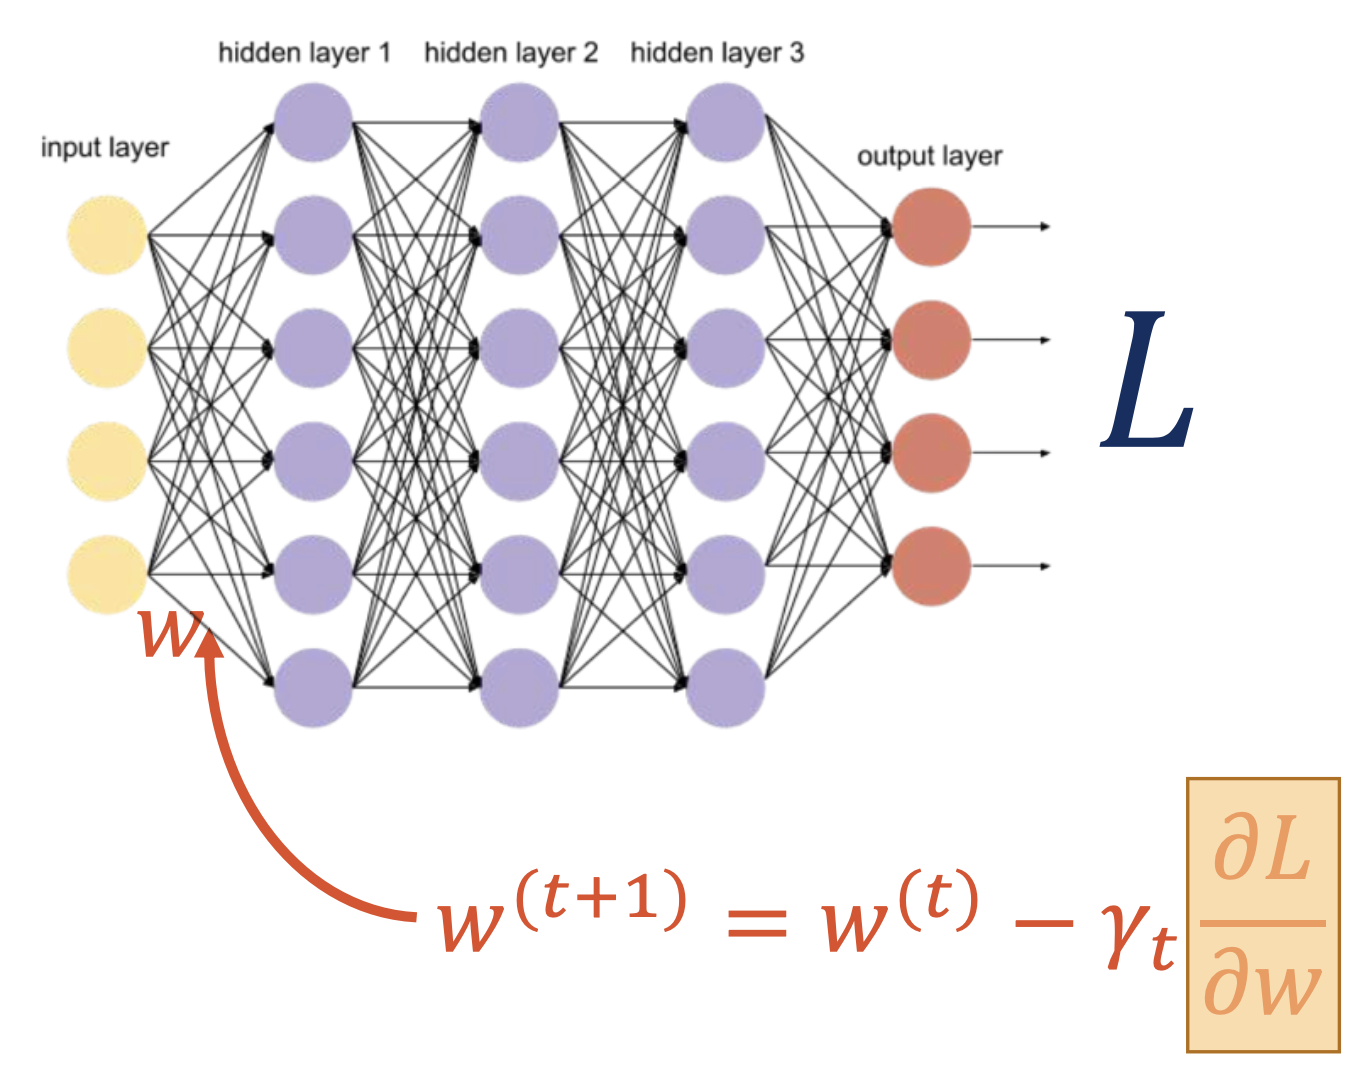
\includegraphics[width=0.45\linewidth]{images/train_1.png}\\
\begin{itemize}
	\small
\setbeamertemplate{items}{\mybullet}
%\item So we know how to update weights
\item So how to find partial derivatives of loss function with respect to some weight?
\end{itemize}

\begin{textblock*}{0.35\paperwidth}(0.65\paperwidth,0.1\paperheight)
	\footnotesize
	\textcolor{gray}{backprop illustrations from \href{https://github.com/data-mining-in-action/}{\underline{DMIA}}}
\end{textblock*}

\end{frame}

%------------------------------------------------

\begin{frame}
\myframetitle{0.22\paperwidth}{0.04\paperwidth}{\insertsection}
\myframesubtitle{0.23\paperwidth}{\insertsubsection}
\centering
\vspace{2.cm}
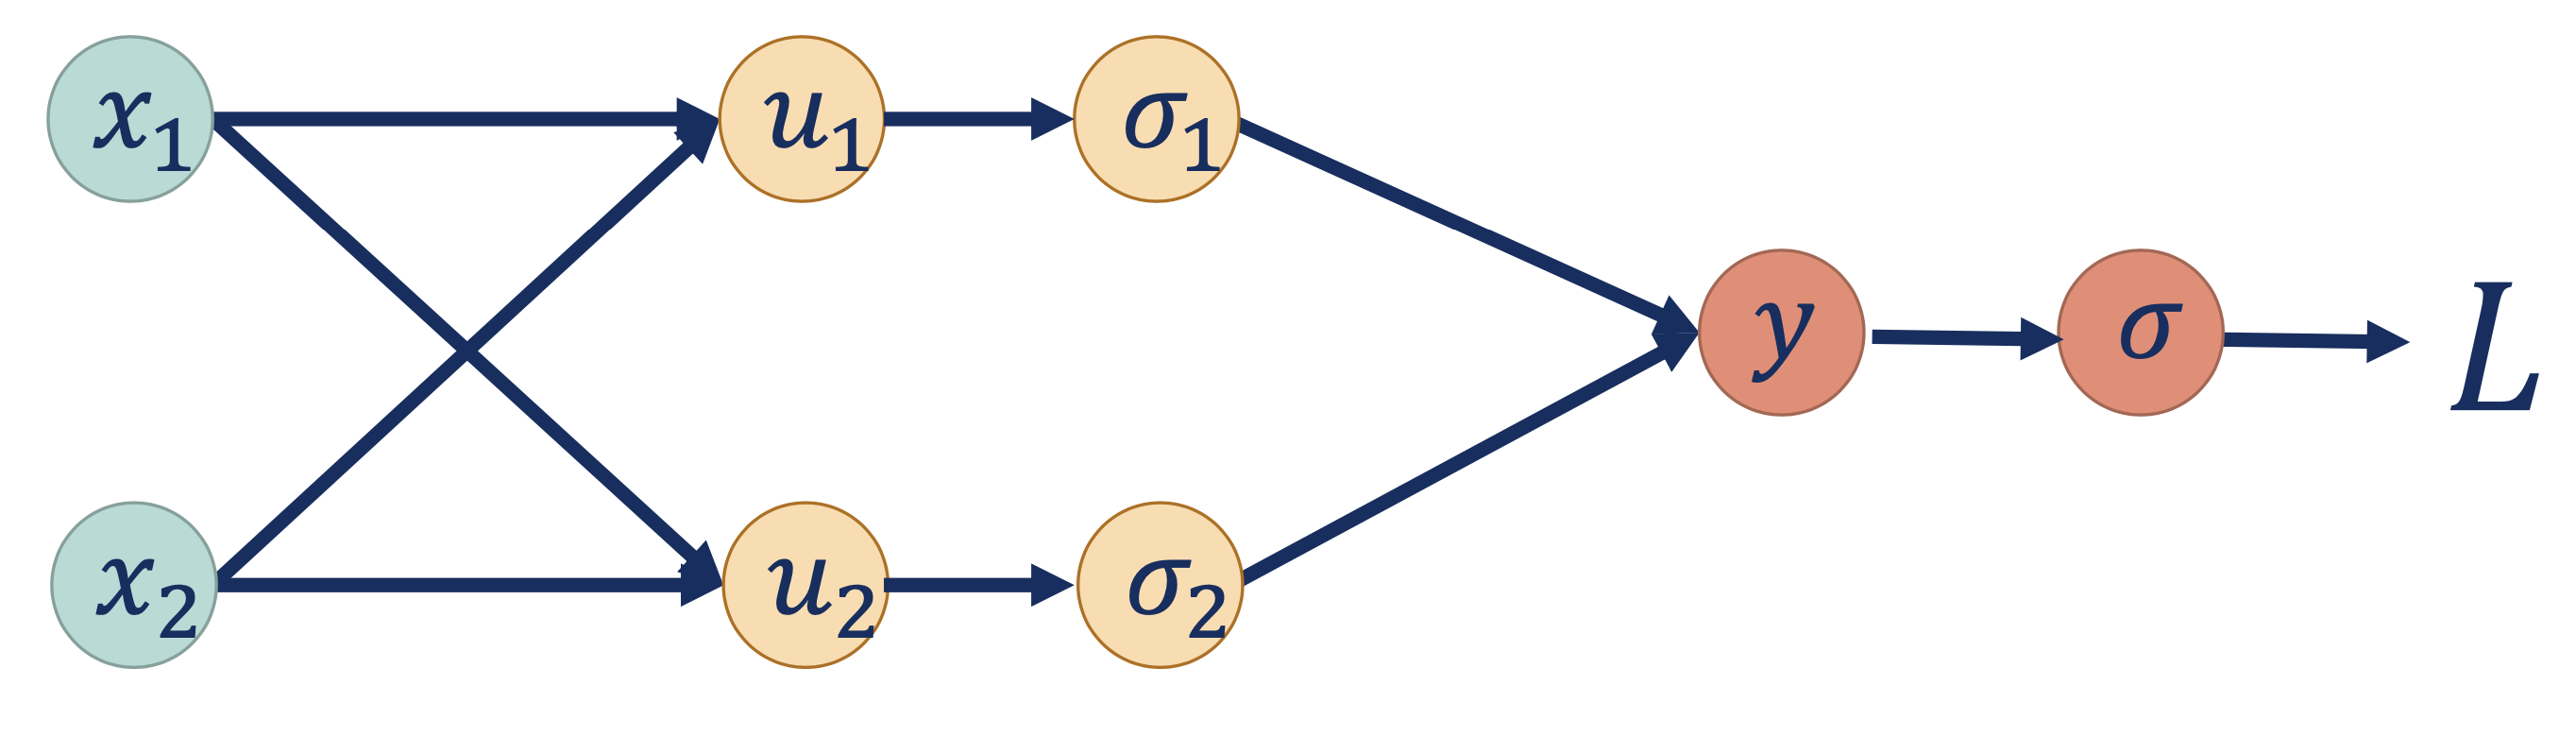
\includegraphics[width=0.8\linewidth]{images/train_2.png}
\vspace{5mm}
\begin{itemize}
	\small
\setbeamertemplate{items}{\mybullet}
\item Let's consider a simplified neural network
\item Represent it in the form of a \textbf{computational graph}
\end{itemize}

\begin{textblock*}{0.35\paperwidth}(0.65\paperwidth,0.1\paperheight)
	\footnotesize
	\textcolor{gray}{backprop illustrations from \href{https://github.com/data-mining-in-action/}{\underline{DMIA}}}
\end{textblock*}
\end{frame}

%------------------------------------------------

\begin{frame}
\myframetitle{0.22\paperwidth}{0.04\paperwidth}{\insertsection}
\myframesubtitle{0.23\paperwidth}{\insertsubsection}
\centering
\vspace{2.3cm}
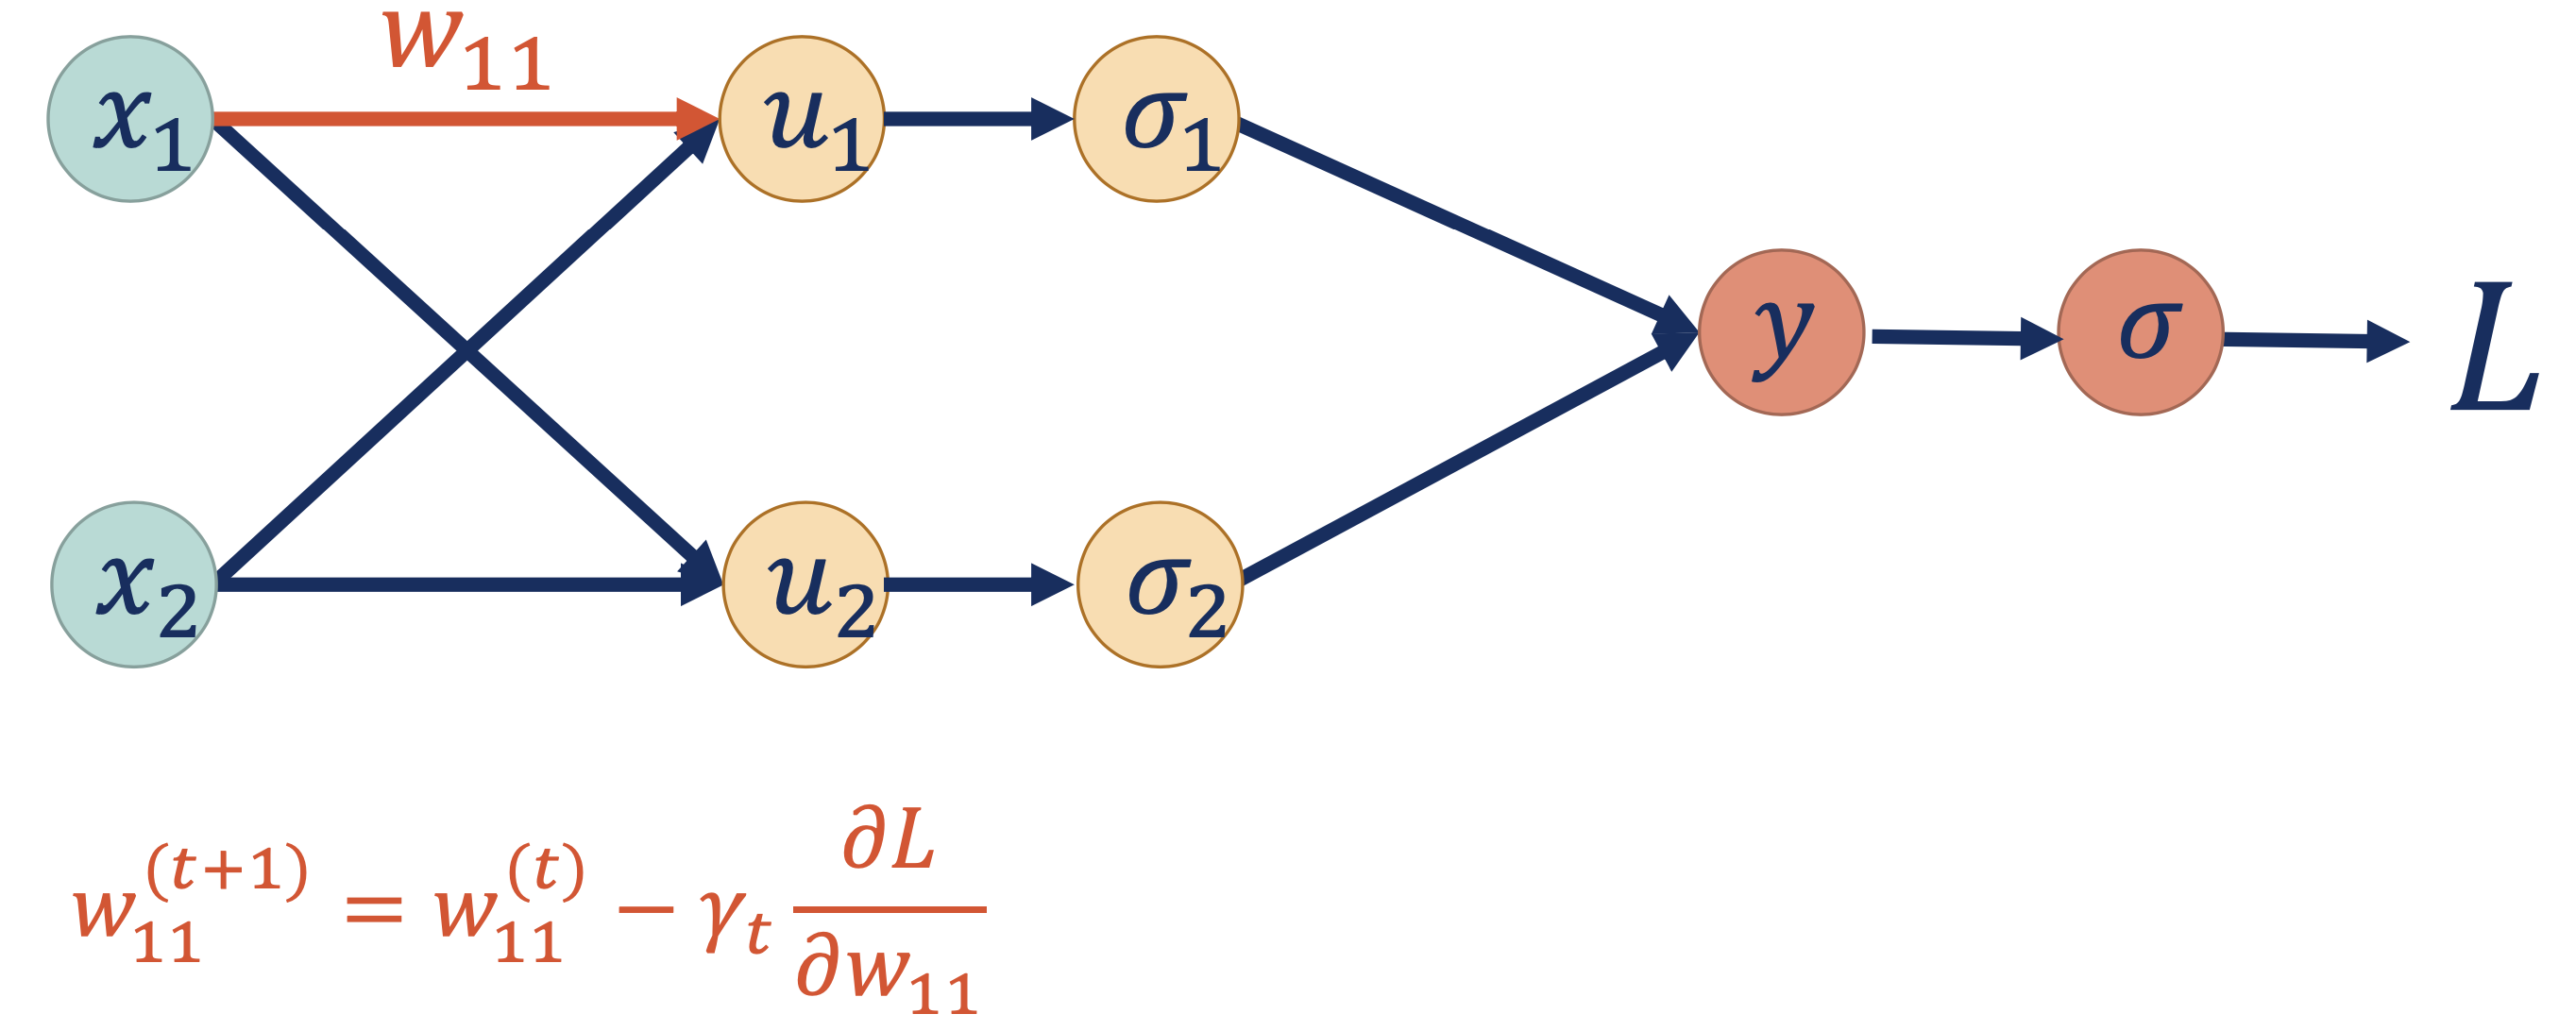
\includegraphics[width=0.8\linewidth]{images/train_3.png}\\
%\begin{itemize}
%\item {We know how to update a weight}
%\end{itemize}
\end{frame}

%------------------------------------------------

\begin{frame}
\myframetitle{0.22\paperwidth}{0.04\paperwidth}{\insertsection}
\myframesubtitle{0.23\paperwidth}{\insertsubsection}
\centering
\vspace{2.3cm}
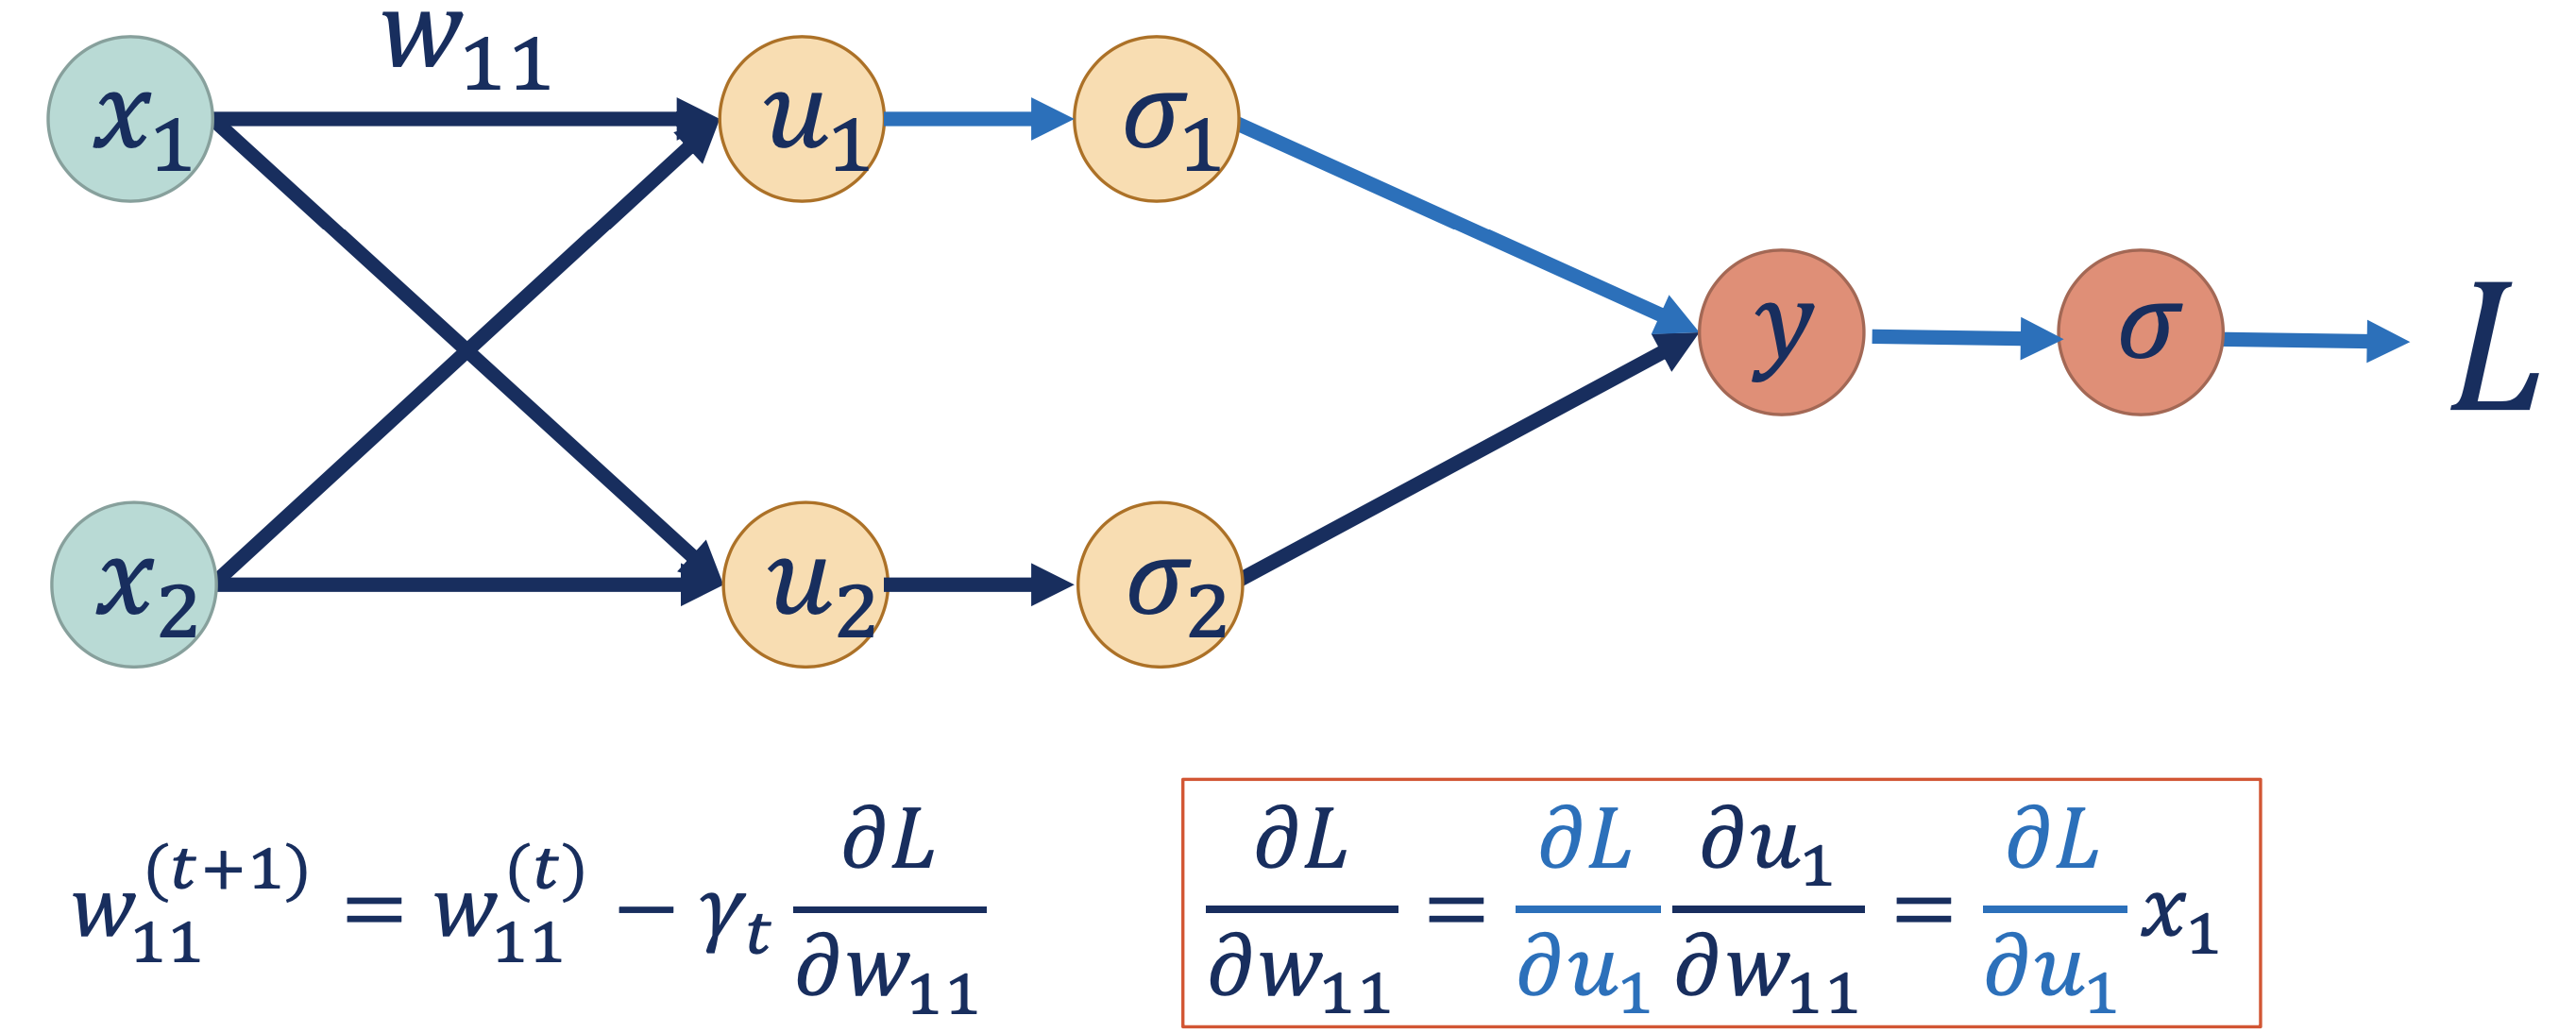
\includegraphics[width=0.8\linewidth]{images/train_4.png}\\
%\begin{itemize}
%\item {We know how to find the partial derivative of the loss function with respect to some weight}
%\end{itemize}
\end{frame}

%------------------------------------------------

\begin{frame}
\myframetitle{0.22\paperwidth}{0.04\paperwidth}{\insertsection}
\myframesubtitle{0.23\paperwidth}{\insertsubsection}
\centering
\vspace{2.3cm}
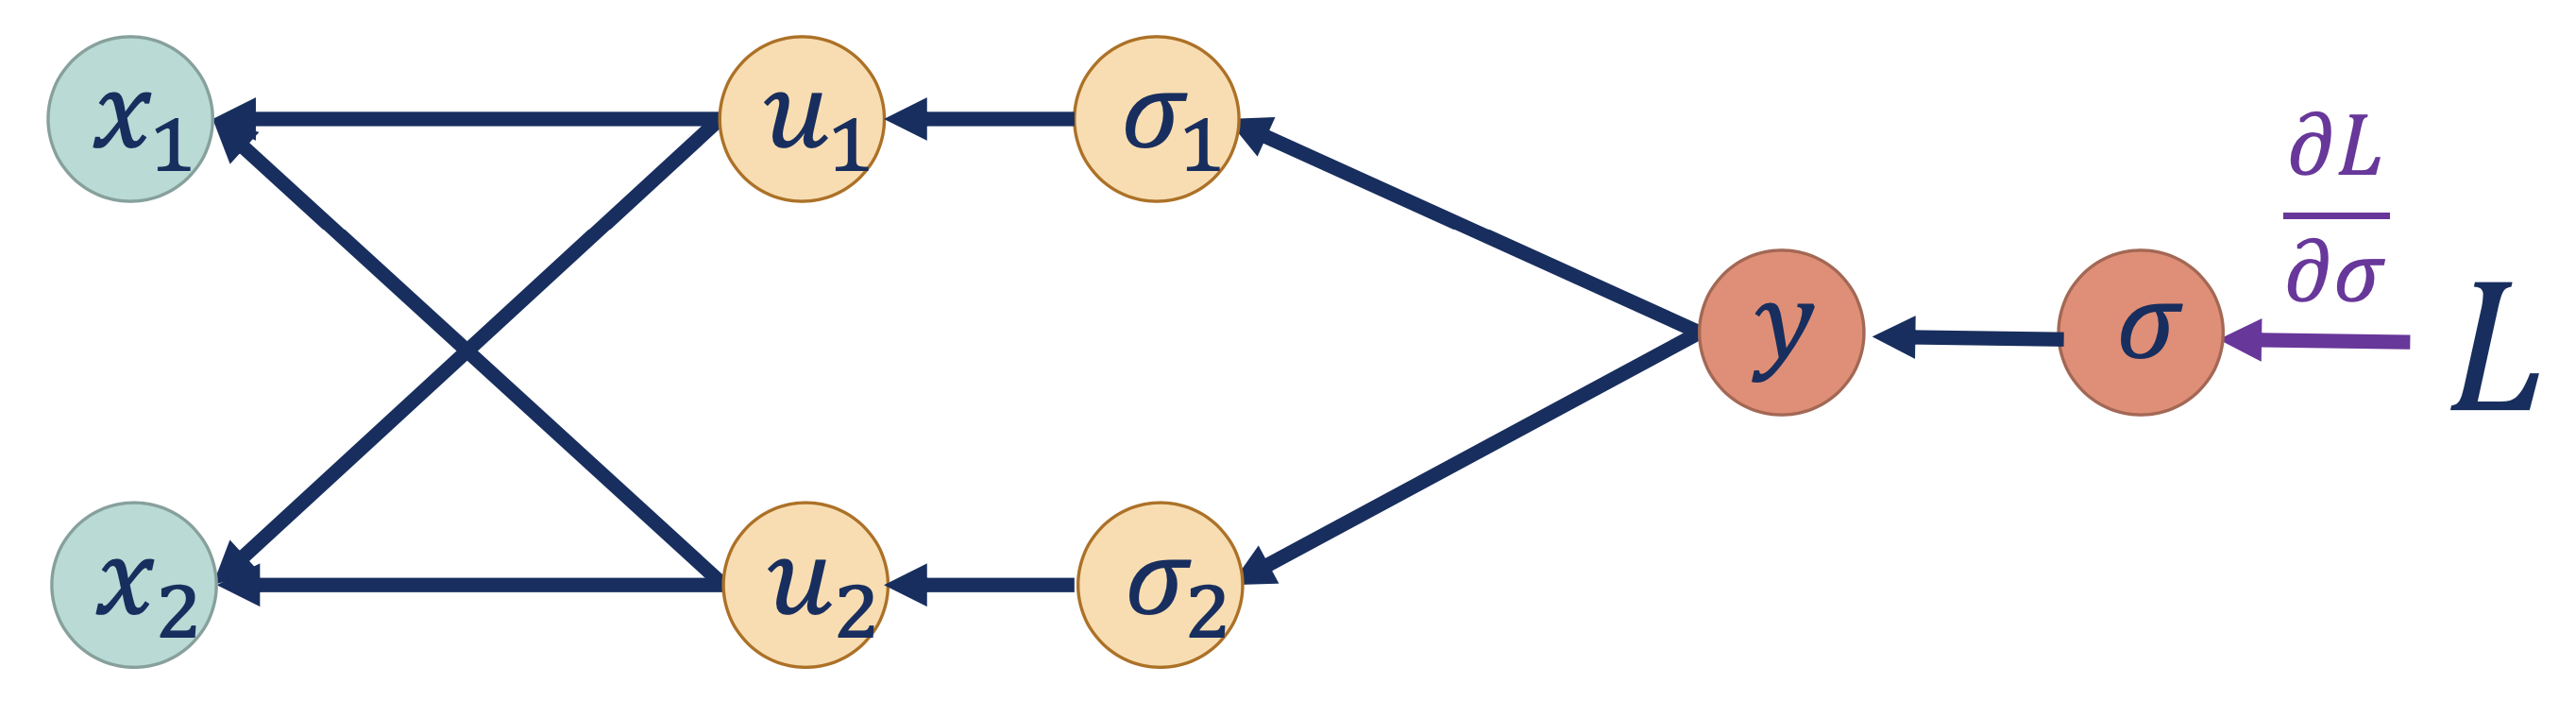
\includegraphics[width=0.8\linewidth]{images/train_5.png}\\
%\begin{itemize}
%\item {Let's try to apply our knowledge to this simple neural network}
%\end{itemize}
\end{frame}

%------------------------------------------------

\begin{frame}
\myframetitle{0.22\paperwidth}{0.04\paperwidth}{\insertsection}
\myframesubtitle{0.23\paperwidth}{\insertsubsection}
\centering
\vspace{2.3cm}
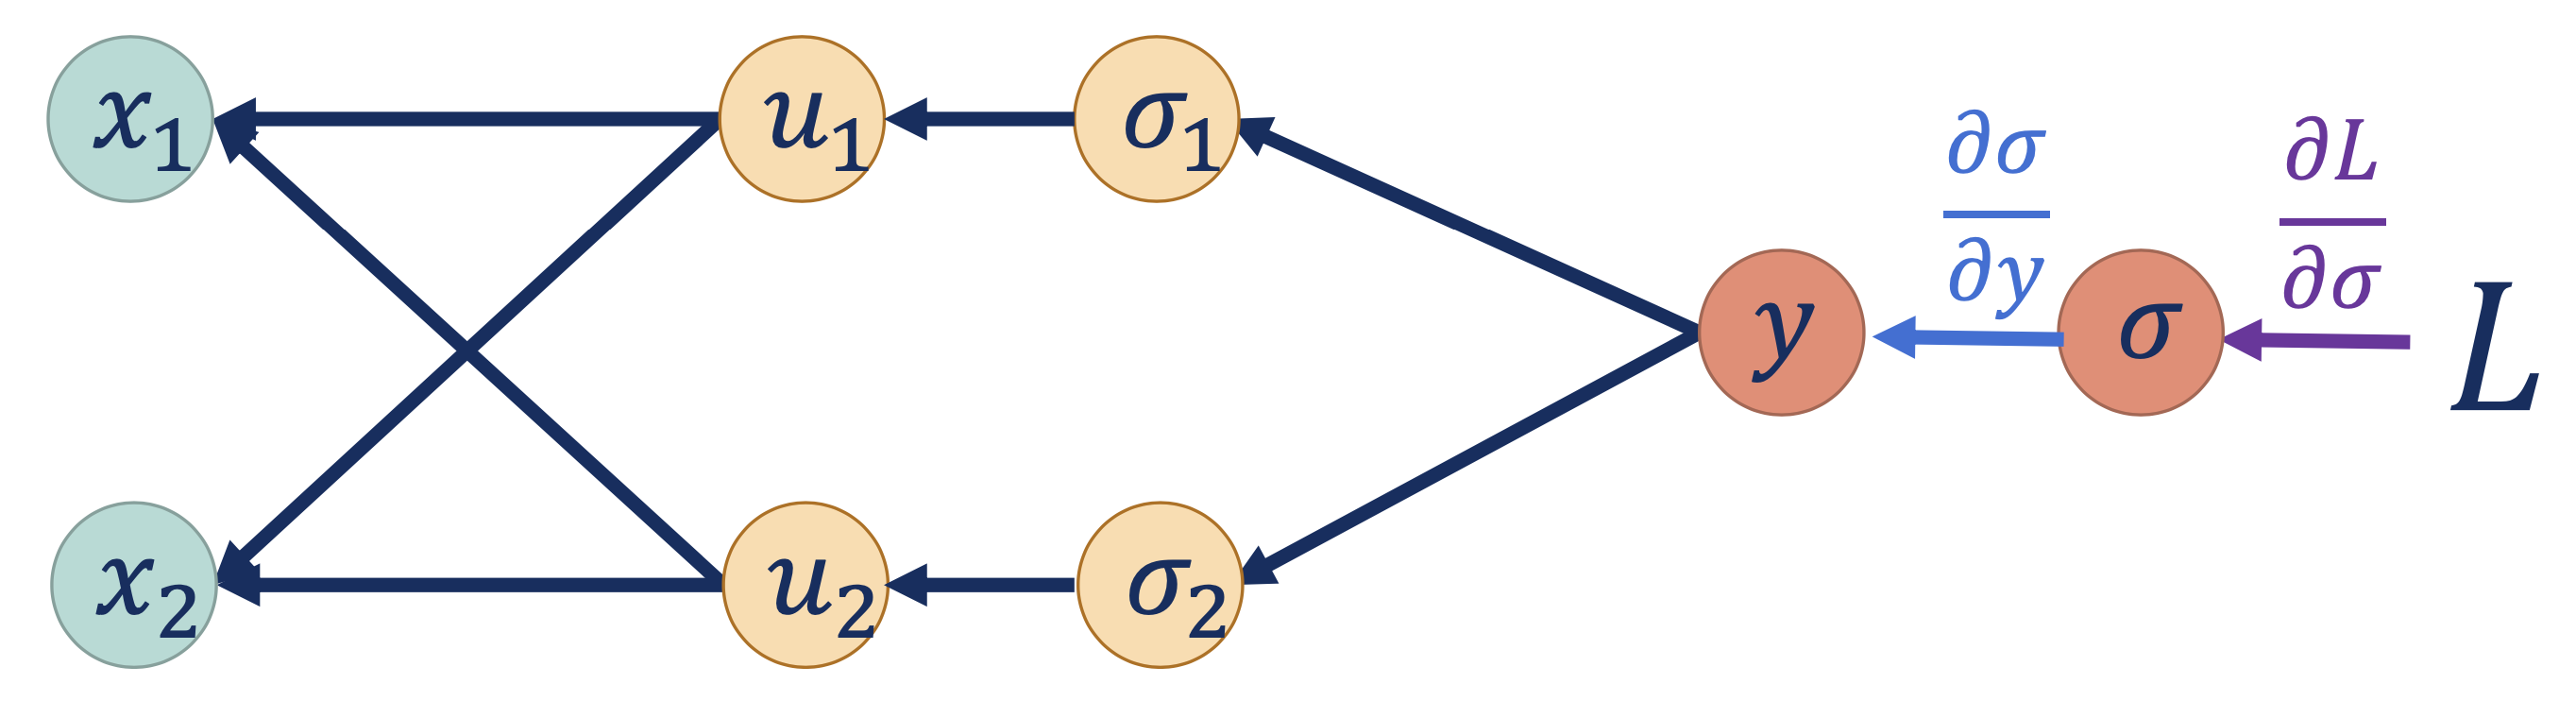
\includegraphics[width=0.8\linewidth]{images/train_6.png}\\
%\begin{itemize}
%\item {Going back over the network to the beginning}
%\end{itemize}
\end{frame}

%------------------------------------------------

\begin{frame}
\myframetitle{0.22\paperwidth}{0.04\paperwidth}{\insertsection}
\myframesubtitle{0.23\paperwidth}{\insertsubsection}
\centering
\vspace{2.3cm}
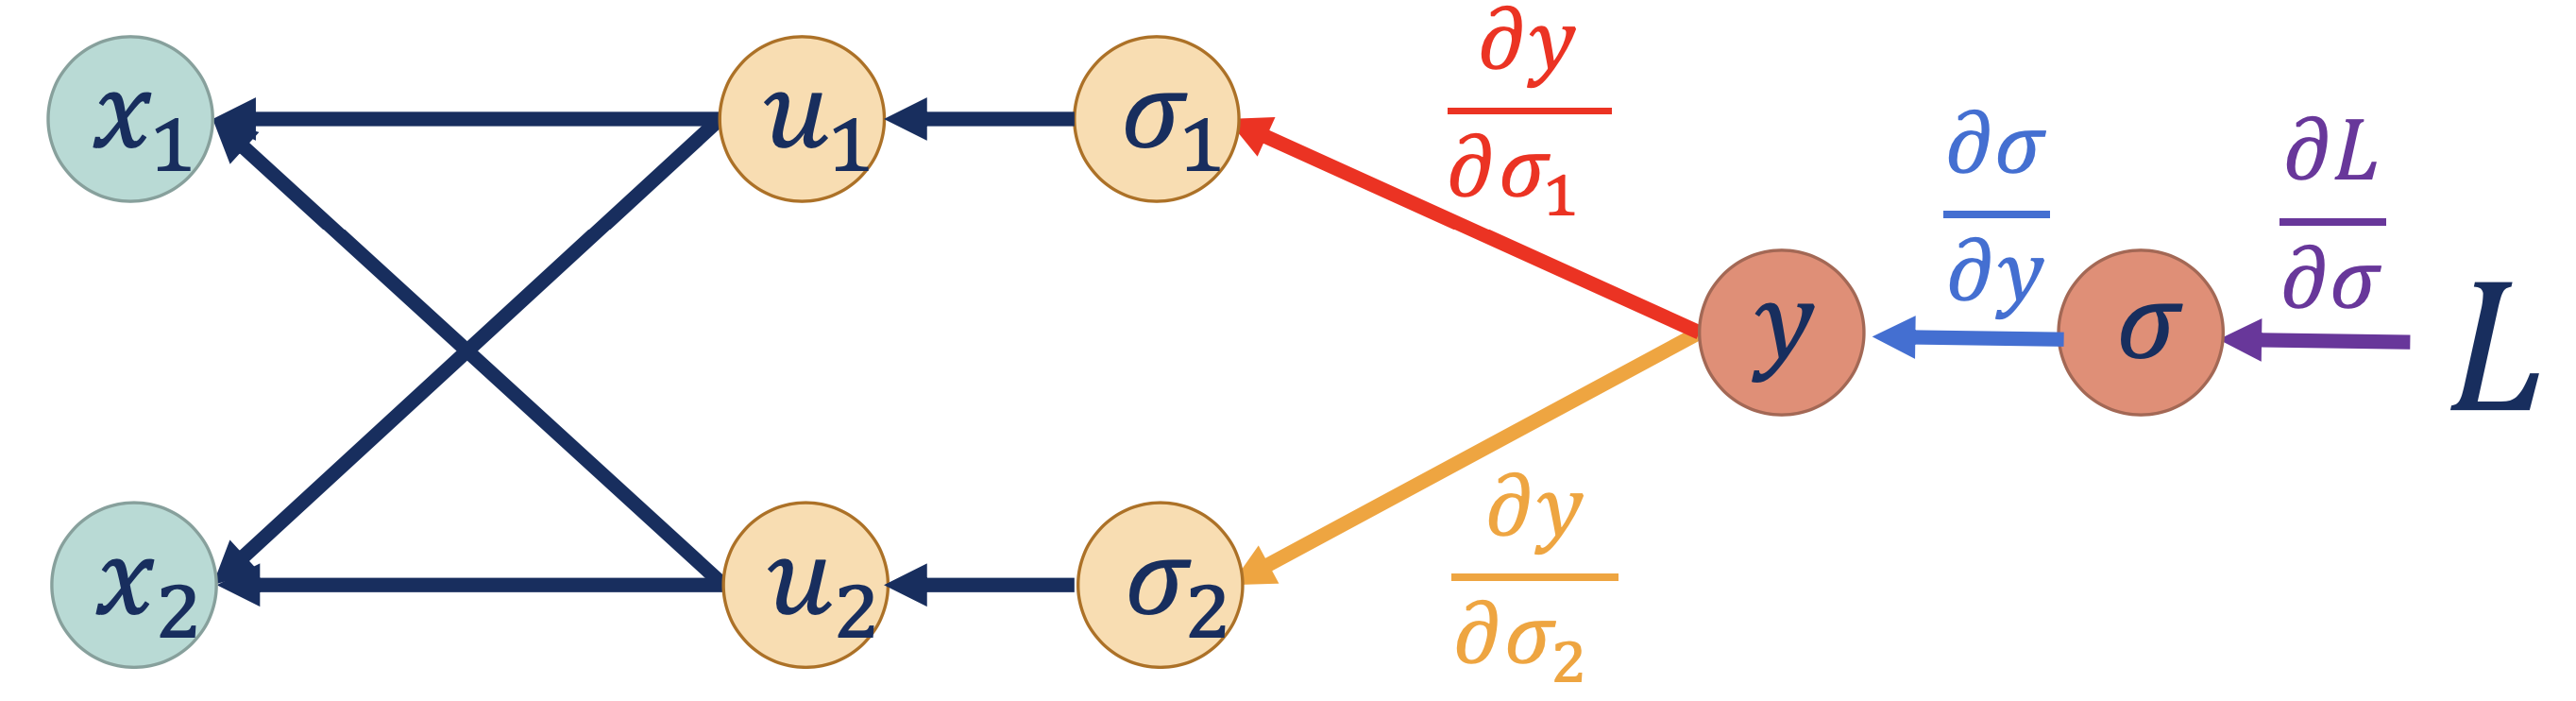
\includegraphics[width=0.8\linewidth]{images/train_7.png}\\
%\begin{itemize}
%\item {Let's go further to the beginning}
%\end{itemize}
\end{frame}

%------------------------------------------------

\begin{frame}
\myframetitle{0.22\paperwidth}{0.04\paperwidth}{\insertsection}
\myframesubtitle{0.23\paperwidth}{\insertsubsection}
\centering
\vspace{2.3cm}
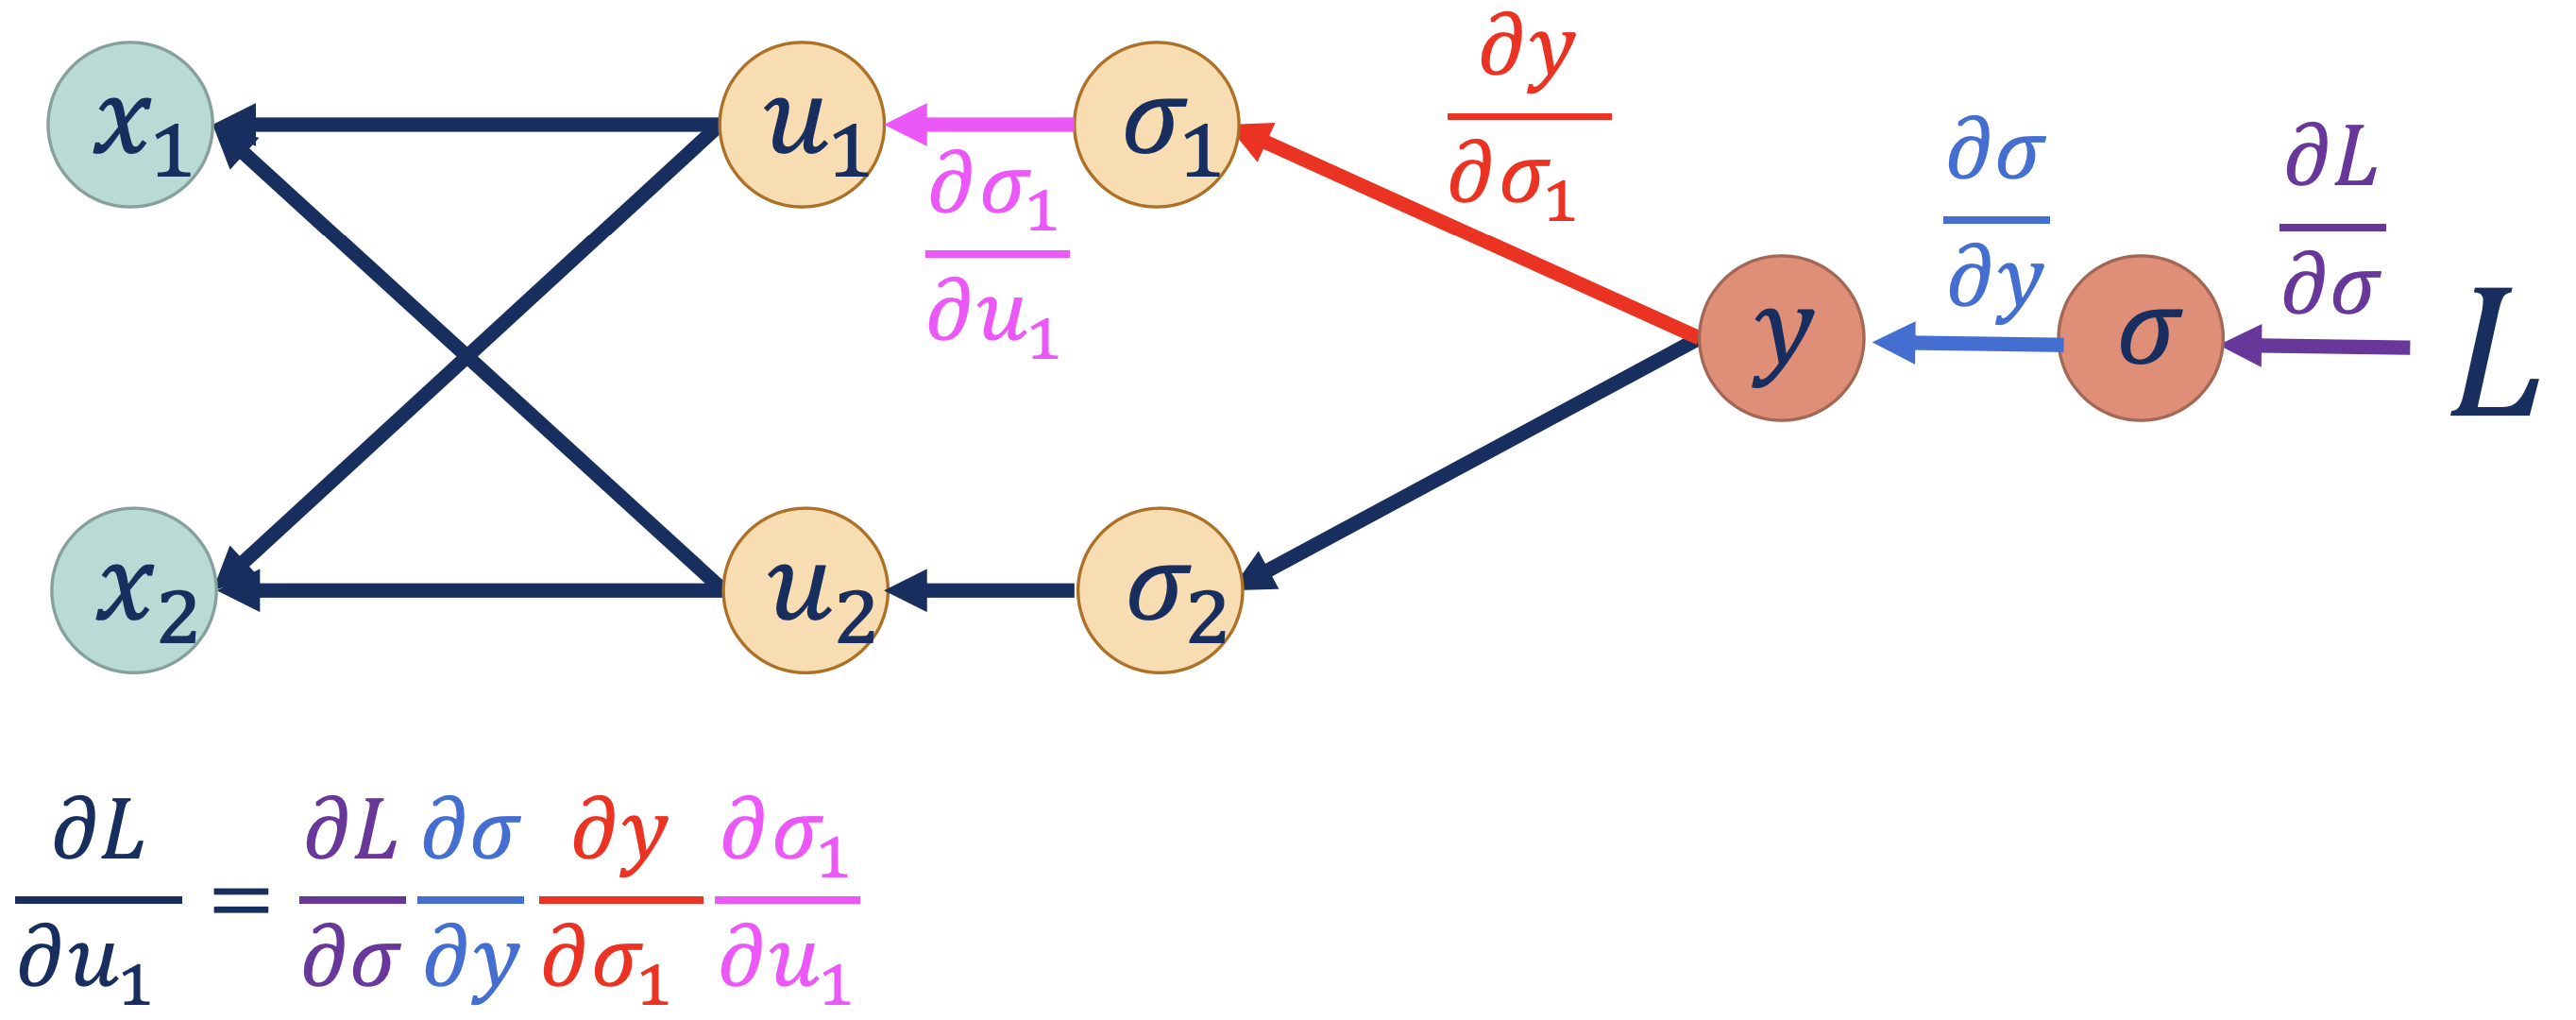
\includegraphics[width=0.8\linewidth]{images/train_8.png}\\
%\begin{itemize}
%\item {Now we know the value of the partial derivative of the loss function with respect to some weight}
%\end{itemize}

\begin{textblock*}{0.55\linewidth}(0.5\paperwidth, 0.68\paperheight)
	\small
	\only<2->{
	\begin{itemize}
		\footnotesize
		\item this procedure is called \textbf{backpropagation}
		\item its idea is to \textbf{collect derivatives} at each step in the computational graph w/o recalculating them every single time for every weight
	\end{itemize}
	}
\end{textblock*}

\end{frame}

%------------------------------------------------

\subsection{wrap it up}
\begin{frame}
\myframetitle{0.22\paperwidth}{0.04\paperwidth}{\insertsection}
\myframesubtitle{0.23\paperwidth}{\insertsubsection}
\centering
\vspace{0.61\paperheight}
\begin{textblock*}{0.8\textwidth}(0.1\paperwidth, 0.2\paperheight)
	\includegraphics<1>[width=0.8\linewidth]{images/train_9.png}
	\includegraphics<2>[width=0.8\linewidth]{images/train_10.png}
	\includegraphics<3>[width=0.8\linewidth]{images/train_3.png}
	\includegraphics<4->[width=0.8\linewidth]{images/train_9.png}
\end{textblock*}


\begin{enumerate}
	\footnotesize
	\item<1-> make \textbf{forward pass} through NN to calculate the output of each neuron and value of loss function
	\item<2-> with \textbf{backward pass} go back through NN to calculate gradients for all weights
	\item<3-> update weights with their gradients
	\item<4-> repeat until convergence
	\item<4->[] *one iteration (\textbf{epoch}) = forward and backward pass
\end{enumerate}

\begin{textblock*}{0.45\paperwidth}(0.6\paperwidth,0.1\paperheight)
	\footnotesize
	\href{https://playground.tensorflow.org/}{\textcolor{gray}{\underline{train NN in your browser!}}}
\end{textblock*}

\end{frame}

%------------------------------------------------
%------------------------------------------------
\section{Going deeper}
%------------------------------------------------
%------------------------------------------------

\begin{frame}[plain]
\centering
\huge

%\begin{textblock*}{0.3\paperwidth}(0.25\paperwidth,0.3\paperheight)
\centering
\vspace{0.1\paperheight}
\begin{tcolorbox}[colframe=white, colback=mygrey, width=0.4\paperwidth,
	arc=2.mm, boxsep=2mm,
	box align=center,
	halign=center,
	valign=center,
	]
	\insertsection
\end{tcolorbox}

%\end{textblock*}

\transfade[duration=.4]
\end{frame}

%------------------------------------------------

\subsection{universal approximation theorem }
\begin{frame}

\myframetitle{0.29\paperwidth}{0.04\paperwidth}{\insertsection}
\myframesubtitle{0.3\paperwidth}{\insertsubsection}

\vspace{0.2\paperheight}
\begin{columns}
	\column{0.7\textwidth}
	\begin{itemize}
		\setbeamertemplate{items}{\mybullet}
		\itemsep1.ex
		\item Roughly speaking, any well-behaved function $f$ can be approximated \textbf{arbitrarily close} with a 1-hidden layer NN, given wide enough hidden layer
		\item  But in practice this is often not the case:
		\begin{itemize}
			\setbeamertemplate{items}{\mysubbullet}
			\item loss function is heavily non-convex
			\item overfitting
			\item not straightforward how to find this NN
		\end{itemize}
	\end{itemize}

	\column{0.3\textwidth}
	\centering
	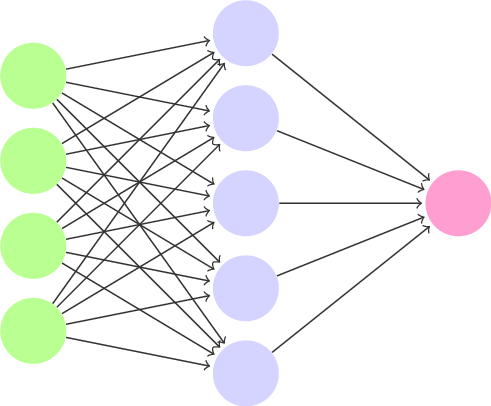
\includegraphics[width = 0.9\textwidth]{nn}
\end{columns}

\end{frame}

%------------------------------------------------

\subsection{stack more layers}
\begin{frame}

\myframetitle{0.29\paperwidth}{0.04\paperwidth}{\insertsection}
\myframesubtitle{0.3\paperwidth}{\insertsubsection}

\vspace{0.15\paperheight}
\begin{itemize}
	\small
	\setbeamertemplate{items}{\mybullet}
	\item<1-> In practice stacking more layers generally \textbf{improves performance}
	\item<2-> Much more layers...
	\item<3-> Which is reminiscent of the \textbf{brain structure}
	\item<3-> Signals travel through multiple areas of different organization
	\item<3-> This makes our perception system incredibly advanced in understanding reality
	\item<4->[\textcolor{myorange}{\MVRightArrow}] \textcolor{myorange}{but there are some problems...}
\end{itemize}

\begin{textblock*}{0.9\paperwidth}(0.05\paperwidth,0.45\paperheight)
	\centering
	\includegraphics<1>[width = 0.5\textwidth]{DNN}
	\includegraphics<2>[width = 0.7\textwidth]{google_net}
	\includegraphics<2>[width = 0.2\textwidth]{more_layers}
\end{textblock*}

\begin{textblock*}{0.9\paperwidth}(0.05\paperwidth,0.62\paperheight)
	\centering
\includegraphics<3>[width = 0.3\textwidth]{visual_stream}
\end{textblock*}

%\includegraphics<1>[width = 0.7\textwidth]{google_net}
%\includegraphics<1>[width = 0.7\textwidth]{DNN}
%\includegraphics<1>[width = 0.3\textwidth]{more_layers}
%\includegraphics<2->[width = 0.3\textwidth]{visual_stream}

\begin{textblock*}{0.45\paperwidth}(0.65\paperwidth,0.1\paperheight)
	\footnotesize
	\href{https://arxiv.org/pdf/1409.4842.pdf}{\textcolor{gray}{\underline{Going deeper with convolutions}}}
\end{textblock*}


\end{frame}
%------------------------------------------------

\subsection{vanishing gradients}
\begin{frame}

\myframetitle{0.29\paperwidth}{0.04\paperwidth}{\insertsection}
\myframesubtitle{0.3\paperwidth}{\insertsubsection}

\vspace{0.15\paperheight}
\begin{columns}
	\column{0.62\textwidth}
	\begin{itemize}
		\small
		\setbeamertemplate{items}{\mybullet}
			\item Layer $f_i(\bm{z_{i-1}})$ takes the output $\bm{z_{i-1}}$ from the previous layer and returns $\bm{z_i}$
			\item Using chain rule and sigmoid activation we have:\\$\Delta \omega_j \sim \cfrac{\partial Q}{\partial \omega_j} = \cfrac{\partial Q}{\partial f_i}\cfrac{\partial f_i}{\partial f_{i-1}}\cdots \cfrac{\partial f_{1}}{\partial \omega_j}$\\
			$\cfrac{\partial f_i}{\partial f_{i-1}} = \sigma(z_{i-1})\big(1-\sigma(z_{i-1})\big)$
			\item $\bigg|\cfrac{\partial f_i}{\partial f_{i-1}}\bigg| \leq \cfrac{1}{4} \Rightarrow \cfrac{\partial Q}{\partial \omega_j} \lesssim \left(\cfrac{1}{4}\right)^n \Rightarrow \boldsymbol{\Delta \omega_j \rightarrow 0, \, n \rightarrow \infty}$
			\vspace{2ex}
			\item[\textcolor{myorange}{\MVRightArrow}] \textcolor{myorange}{there's no learning happening}
%		\item<2->[\textcolor{myorange}{\MVRightArrow}] \textcolor{myorange}{what can be the cause?}
	\end{itemize}	

	\column{0.5\textwidth}
	\centering
	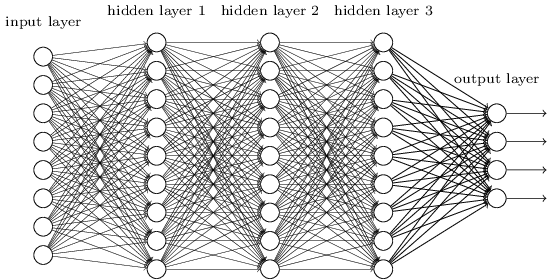
\includegraphics[width=0.6\linewidth]{DNN}
	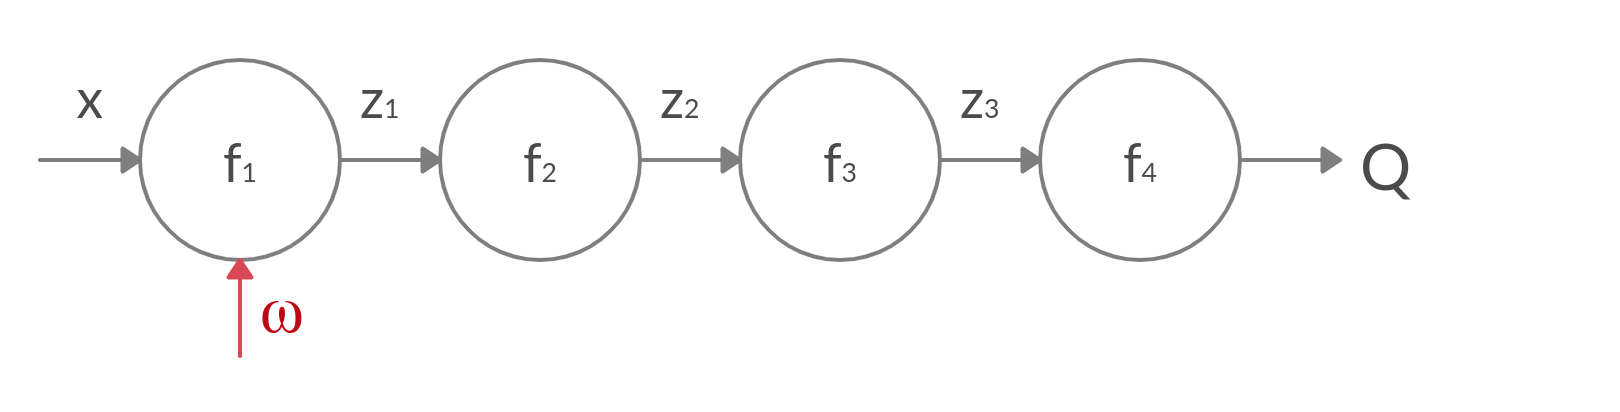
\includegraphics[width=1\linewidth]{vanishing_grad_NN}
	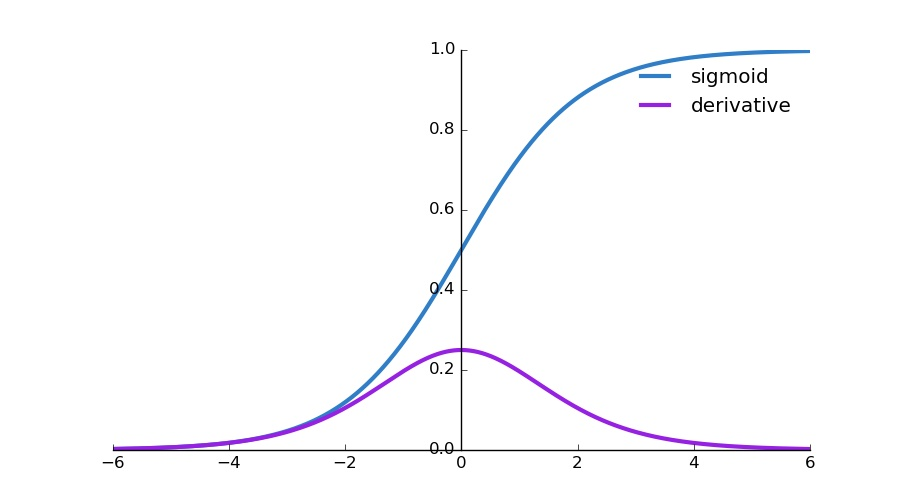
\includegraphics[width=0.6\linewidth]{sigmoid_der}
	
\end{columns}


\end{frame}

%------------------------------------------------

\subsection{activation functions}
\begin{frame}

\myframetitle{0.29\paperwidth}{0.04\paperwidth}{\insertsection}
\myframesubtitle{0.3\paperwidth}{\insertsubsection}

\vspace{0.17\paperheight}
\begin{columns}
	\column{0.6\textwidth}
	\begin{itemize}
		\small
		\item[\mybullet] Let's have a closer look at sigmoid activation:
		\[
		\sigma(z) = \dfrac{1}{1+e^{-z}}
		\]
		\item[\textcolor{mygreen}{\MVRightArrow}] outputs are in [0,1] range $\Rightarrow$ "neuron fired" intuition
		\item[\textcolor{myorange}{\MVRightArrow}] outputs are not zero-centered
		\item[\textbf{\MVRightArrow}] \textbf{saturate at large $|z|$ $\Rightarrow$ kill gradients} ($\rightarrow0$)
		\item[\mybullet] same applies to $\tanh(z) = \dfrac{e^z - e^{-z}}{e^z + e^{-z}}$
		\vspace{2ex}
		\item<2->[\textcolor{myorange}{\MVRightArrow}] \textcolor{myorange}{can we use other activation functions?}
	\end{itemize}	
	
	\column{0.5\textwidth}
	\centering                                             
	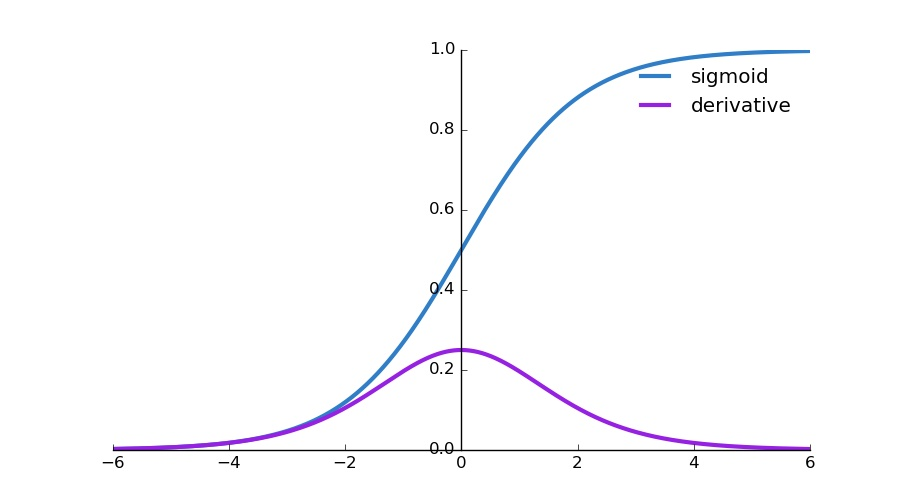
\includegraphics[width=0.8\linewidth]{sigmoid_der.jpg}
	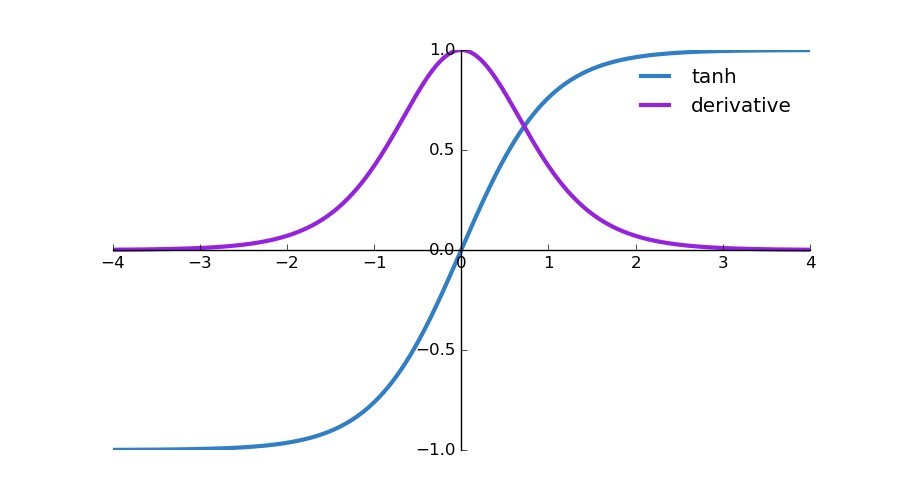
\includegraphics[width=0.9\linewidth]{tan_der.jpg}
\end{columns}

\end{frame}
%------------------------------------------------

\begin{frame}

\myframetitle{0.29\paperwidth}{0.04\paperwidth}{\insertsection}
\myframesubtitle{0.3\paperwidth}{\insertsubsection}

\vspace{0.25\paperheight}
\begin{itemize}
	\setbeamertemplate{items}{\mybullet}
	\itemsep1.2ex
	\small
	\item<1-> \textcolor{NavyBlue}{ReLU(x)} $=\max(0,z)$
	\begin{itemize}
		\small
		\item[\textcolor{mygreen}{\MVRightArrow}] gradients don't vanish
		\item[\textcolor{mygreen}{\MVRightArrow}] simple implementation (derivative either 0 or 1)
		\item[\textcolor{myorange}{\MVRightArrow}] not zero-centered and unbounded
		\item[\textcolor{myorange}{\MVRightArrow}] neurons can "die"
		\item[\textcolor{myblack}{\MVRightArrow}] there's more: Leaky ReLU, ELU, GELU, Softplus
	\end{itemize}
	\item and even  \href{https://arxiv.org/pdf/1710.05941.pdf}{\textcolor{gray}{\underline{more}}}:
	\item[] e.g., \textcolor{Rhodamine}{Swish(z)} $= \cfrac{z}{1+e^{-\beta \cdot z}} = z \cdot \sigma(\beta \cdot z)$
\end{itemize}

%\vspace{5mm}
%\footnotesize
%\textcolor{myorange}{\textbf{Informal guideline:}} don't use $\sigma(z)$, try ReLU as baseline and then the others

\begin{textblock*}{0.45\paperwidth}(0.67\paperwidth,0.38\paperheight)
	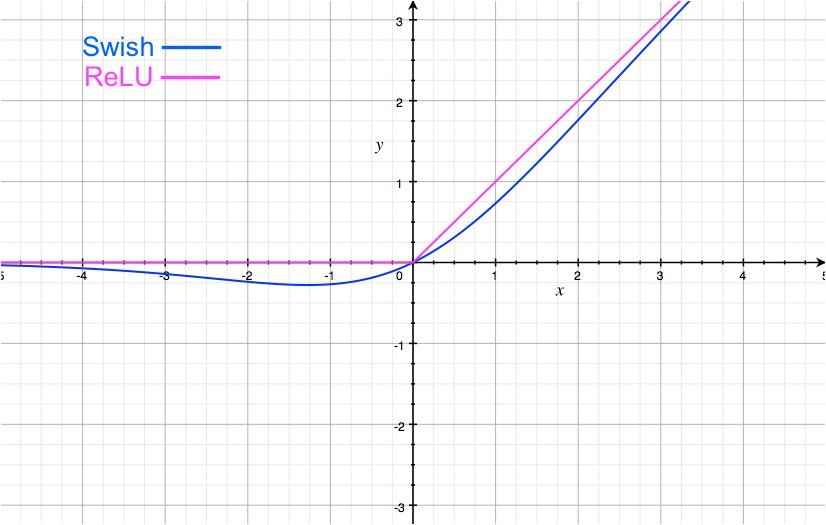
\includegraphics[width=0.7\linewidth]{swish}
\end{textblock*}

\begin{textblock*}{0.45\paperwidth}(0.65\paperwidth,0.1\paperheight)
	\footnotesize
	\href{https://arxiv.org/pdf/1710.05941.pdf}{\textcolor{gray}{\underline{Searching for activation functions}}}
\end{textblock*}

\end{frame}
%------------------------------------------------

\subsection{weight initialisation}
\begin{frame}

\myframetitle{0.29\paperwidth}{0.04\paperwidth}{\insertsection}
\myframesubtitle{0.3\paperwidth}{\insertsubsection}

\begin{textblock*}{0.95\paperwidth}(0.03\paperwidth,0.22\paperheight)
		\begin{itemize}
		\itemsep1.2ex
		\small
		\setbeamertemplate{items}{\mybullet}
		\item But gradients can also \textbf{explode}
		\item<2-> Intuitively, weights are updated by: 
		\vspace{2mm}\\$\Delta \omega_j \sim  \cfrac{\partial Q}{\partial f_i}\cfrac{\partial f_i}{\partial f_{i-1}}\cdots \cfrac{\partial f_{1}}{\partial \omega_j}\sim \prod\limits_{i} S_{ij}$\\
		\vspace{2mm}
		 $S_{ij}$ - scale of gradient at $i$-th layer
		\item<2-> if $S_{ij} \ll 1$, gradients vanish and weights don't update $\Rightarrow$ learning is stuck
		\item<2-> if $S_{ij} \gg 1$, gradients explode $\Rightarrow$ learning is extremely unstable
		\item<3->[] \textcolor{mygreen}{\textbf{Idea:}} constrain the scales at each layer to avoid exponential growth
		\begin{itemize}
			\item<3->[\textcolor{myblack}{\MVRightArrow}] one can \href{https://cs231n.github.io/neural-networks-2/}{\textcolor{gray}{\underline{show}}} that clever weight initialisation can remedy this
		\end{itemize}
	\end{itemize}
\end{textblock*}

\only<3->{
\begin{textblock*}{0.95\paperwidth}(0.12\paperwidth,0.83\paperheight)
	\footnotesize
	\textcolor{myblack}{\MVRightArrow} e.g. \href{http://proceedings.mlr.press/v9/glorot10a/glorot10a.pdf}{\textcolor{gray}{\underline{Xavier}}}: $W_j \sim \mathcal{N}\left(0, \dfrac{1}{n_\text{in}}\right)$ or \href{https://arxiv.org/pdf/1502.01852.pdf}{\textcolor{gray}{\underline{He}}}: $W_j \sim \mathcal{N}\left(0, \dfrac{2}{n_\text{in}}\right)$ (for ReLU) initialisations\textcolor{gray}{*}
\end{textblock*}

\begin{textblock*}{0.15\paperwidth}(0.83\paperwidth,0.75\paperheight)
	\tiny
	\textcolor{gray}{*library implementations may slightly \href{https://pytorch.org/docs/master/nn.init.html}{\underline{differ}}}
\end{textblock*}
}

\begin{textblock*}{0.45\paperwidth}(0.6\paperwidth,0.25\paperheight)
	\includegraphics<2->[width=0.9\linewidth]{vanishing_grad_NN}
\end{textblock*}

\begin{textblock*}{0.45\paperwidth}(0.75\paperwidth,0.1\paperheight)
	\footnotesize
	\href{https://www.deeplearning.ai/ai-notes/initialization/}{\textcolor{gray}{\underline{init playground}}}
\end{textblock*}

\end{frame}


%------------------------------------------------
%------------------------------------------------
\section{Tackling overfitting}
%------------------------------------------------
%------------------------------------------------

\begin{frame}[plain]
\centering
\huge

%\begin{textblock*}{0.3\paperwidth}(0.25\paperwidth,0.3\paperheight)
\centering
\vspace{0.1\paperheight}
\begin{tcolorbox}[colframe=white, colback=mygrey, width=0.55\paperwidth,
	arc=2.mm, boxsep=2mm,
	box align=center,
	halign=center,
	valign=center,
	]
	\insertsection
\end{tcolorbox}

%\end{textblock*}

\transfade[duration=.4]
\end{frame}

%------------------------------------------------

\subsection{complexity}
\begin{frame}

\myframetitle{0.4\paperwidth}{0.04\paperwidth}{\insertsection}
\myframesubtitle{0.41\paperwidth}{\insertsubsection}

\vspace{0.2\paperheight}
\begin{columns}
	\column{0.65\textwidth}
	\begin{itemize}
		\small
		\setbeamertemplate{items}{\mybullet}
		\item NN are higly complicated models with $>1\text{M}$ weights being normal
		\item Therefore, optimisation task is extremely tough with loss function being non-convex 
		\item This makes overfitting and getting trapped in a local minimum a piece of cake 
		\item<2>[\textcolor{myorange}{\MVRightArrow}] \textcolor{myorange}{Improvements in optimisation methods are needed}
	\end{itemize}

	\column{0.4\textwidth}
	\flushright
	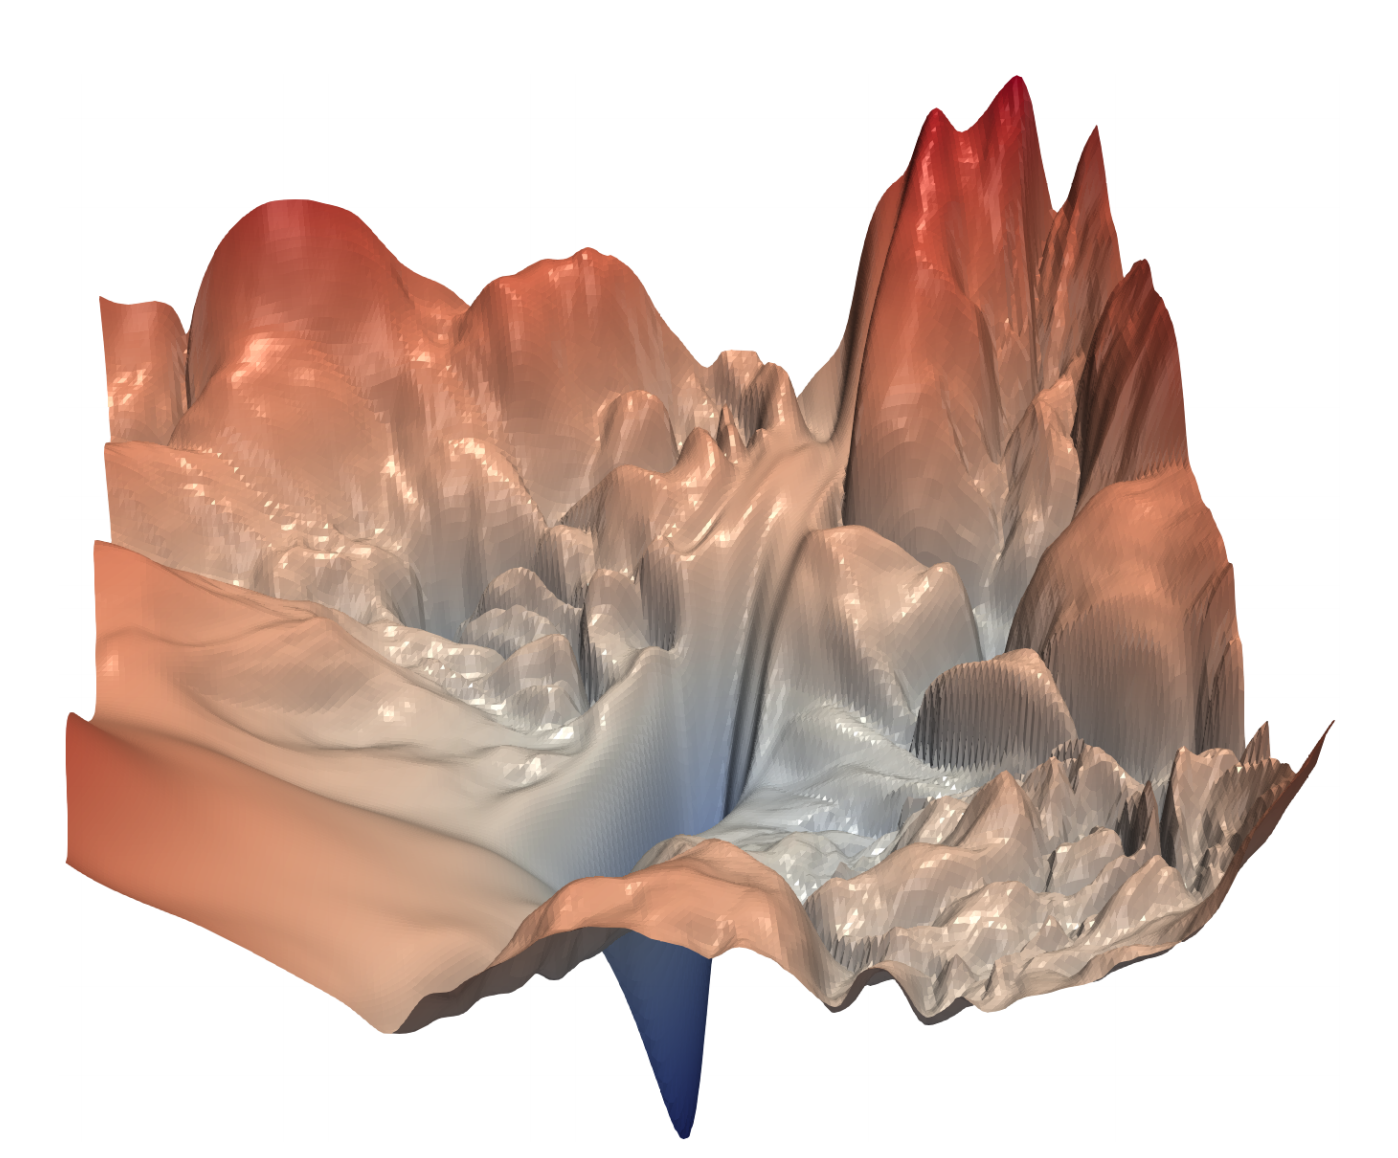
\includegraphics[width=0.9\linewidth]{loss_landscape}
\end{columns}


\begin{textblock*}{0.45\paperwidth}(0.68\paperwidth,0.1\paperheight)
	\footnotesize
	\href{https://papers.nips.cc/paper/7875-visualizing-the-loss-landscape-of-neural-nets}{\textcolor{gray}{\underline{Visualizing the Loss Landscape}}}
\end{textblock*}



\end{frame}

%------------------------------------------------

\subsection{SGD recap}
\begin{frame}

\myframetitle{0.4\paperwidth}{0.04\paperwidth}{\insertsection}
\myframesubtitle{0.41\paperwidth}{\insertsubsection}

\vspace{0.2\paperheight}
\begin{columns}
	\column{0.65\textwidth}
	\begin{itemize}
		\small
		\setbeamertemplate{items}{\mybullet}
		\item \textbf{SGD:}
		\begin{itemize}
			\small
			\setbeamertemplate{items}{\mysubbullet}
			\item At each step k pick random sample $(\bm x_l, y_l)$ 
			\item Update weights:\\
			$\bm{\omega}^{(k)} \leftarrow \bm{\omega}^{(k-1)} - \eta \nabla Q\left(y_l, f_\omega(\bm x_l)\right)\bigg|_{\bm \omega = \bm \omega^{(k-1)}}$
		\end{itemize}
	
		\item \textbf{Mini-batch SGD:}
		\begin{itemize}
			\small
			\setbeamertemplate{items}{\mysubbullet}
			\item Iterate through the dataset in chunks (batches)
			\item Aggregate gradients over the chunk:
			\[
			\bm g = \sum_{l \in B}\nabla Q\left(y_l, f_\omega(\bm x_l)\right)
			\] 
			\item Update the weigths: $\bm{\omega}^{(k)} \leftarrow \bm{\omega}^{(k-1)} - \eta\cdot \bm g$
		\end{itemize}

	\end{itemize}
	
	\column{0.45\textwidth}
	\centering
	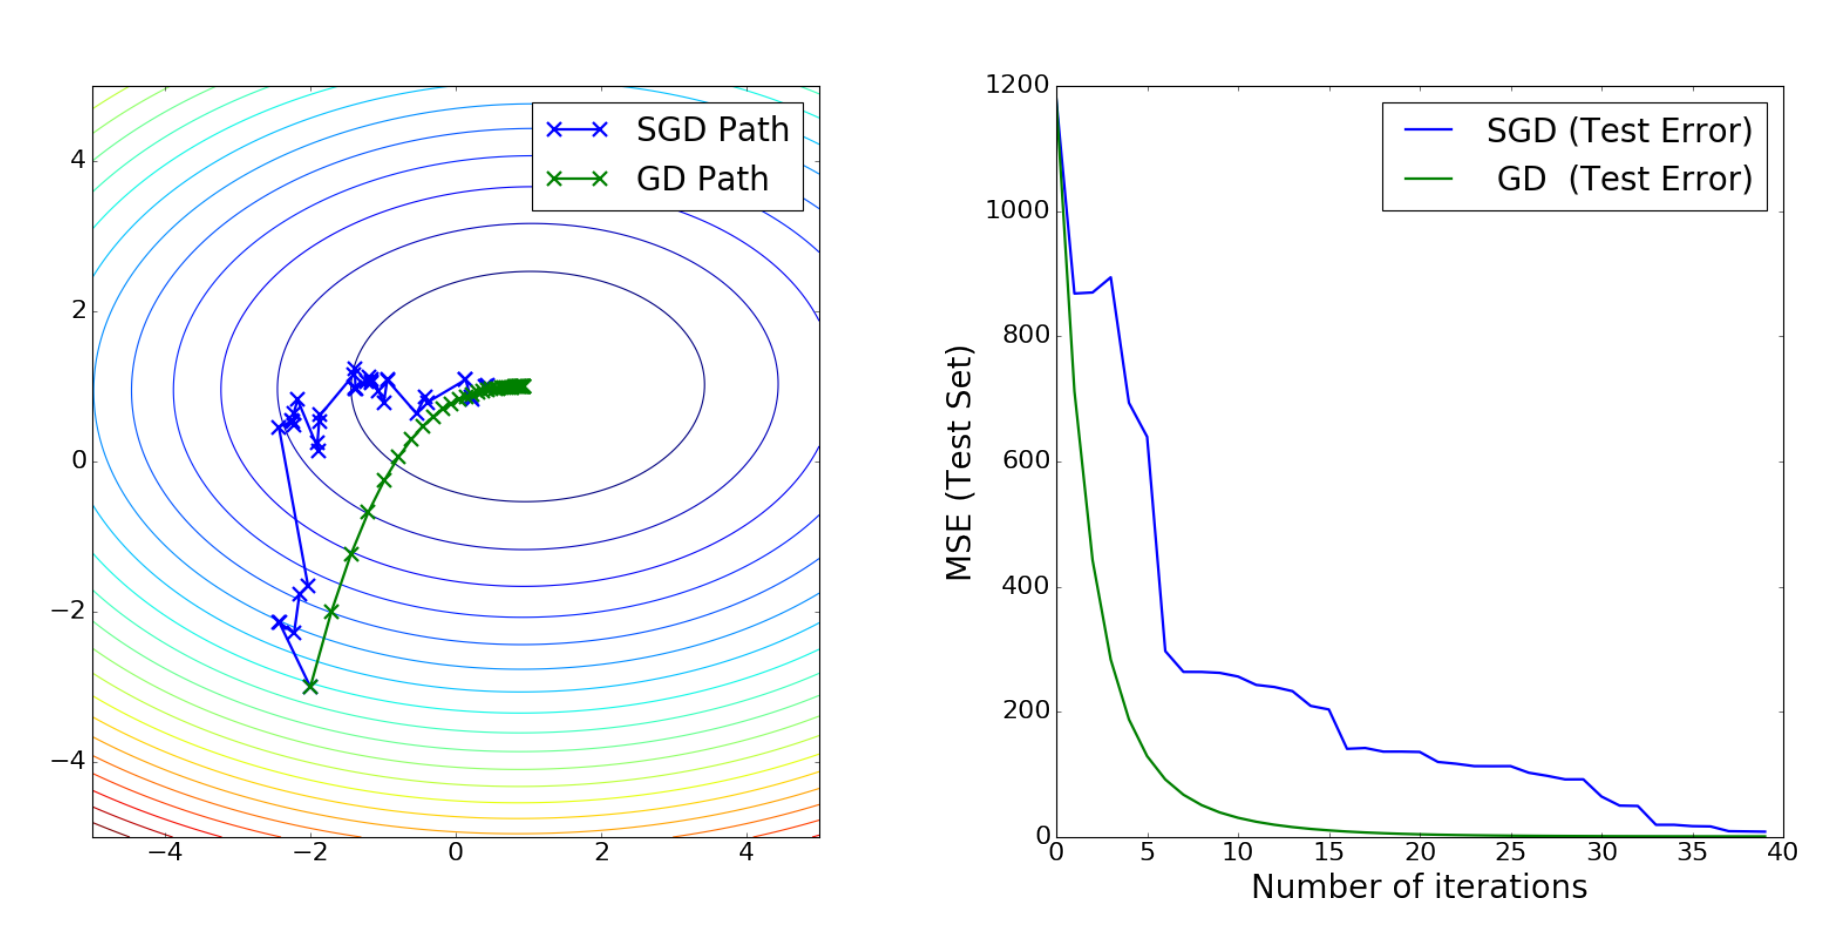
\includegraphics[width=.9\linewidth]{gd_sgd}
	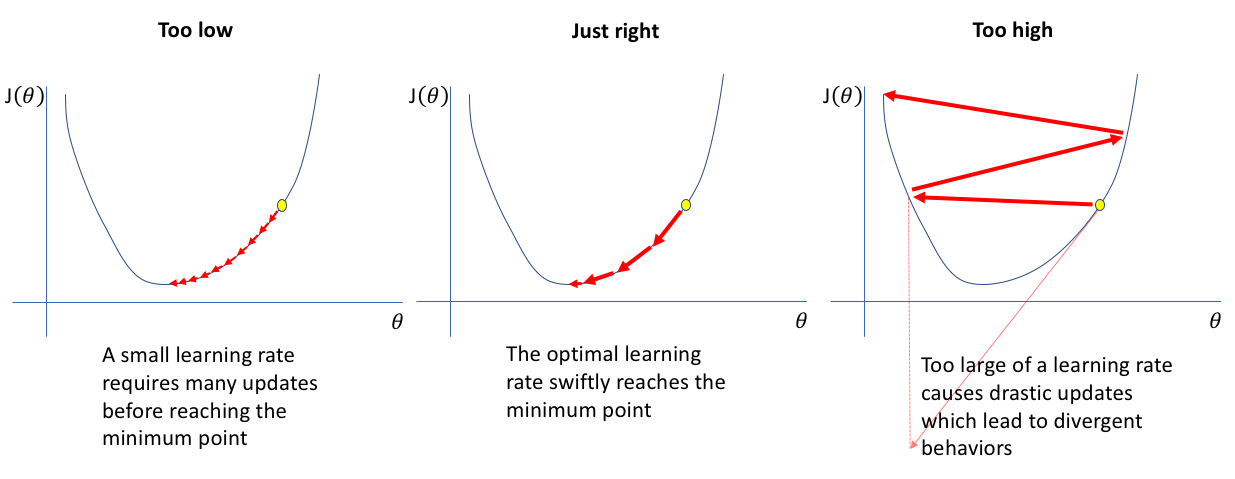
\includegraphics[width=.9\linewidth]{lr_choice}
\end{columns}

\begin{textblock*}{0.45\paperwidth}(0.85\paperwidth,0.11\paperheight)
	\footnotesize
	\href{https://www.cs.ox.ac.uk/people/varun.kanade/teaching/ML-MT2016/lectures/lecture06.pdf}{\textcolor{gray}{\underline{source}}}
\end{textblock*}

\end{frame}

%------------------------------------------------

\subsection{momentum}
\begin{frame}

\myframetitle{0.4\paperwidth}{0.04\paperwidth}{\insertsection}
\myframesubtitle{0.41\paperwidth}{\insertsubsection}

\vspace{0.2\paperheight}
\begin{columns}
	\column{0.65\textwidth}
	\begin{itemize}
		\footnotesize
		\setbeamertemplate{items}{\mybullet}
		\item Let's change perspective to a physical one and add a notion of \textbf{velocity}
		\item Example: a ball rolling down the hill $\Rightarrow$ treat loss as \textbf{potential energy}
		\item If we build up velocity in a direction with consistent gradient, we can overcome local minima and smooth out rapid oscillations $\Rightarrow$ \textbf{SGD with momentum}:
		\[
		\bm{v}^{(k)} \leftarrow \beta \bm{v}^{(k-1)} - \eta \nabla Q\left(y_l, f_\omega(\bm x_l)\right)\bigg|_{\bm \omega = \bm \omega^{(k-1)}}
		\]
		\[
		\bm{\omega}^{(k)} \leftarrow \bm{\omega}^{(k-1)} + \bm{v}^{(k)}
		\]
		\item<2-> \textbf{Nesterov momentum} updates position with \textcolor{mypurple}{"lookahead"} gradient $\nabla Q\left(y_l, f_\omega(\bm x_l)\right)\bigg|_{\bm \omega = \bm \omega^{(k-1)} \textcolor{mypurple}{+ \beta \bm{v}^{(k-1) }}}$
	\end{itemize}
	
	\column{0.5\textwidth}
	
	\begin{textblock*}{0.45\paperwidth}(0.63\paperwidth,0.22\paperheight)
		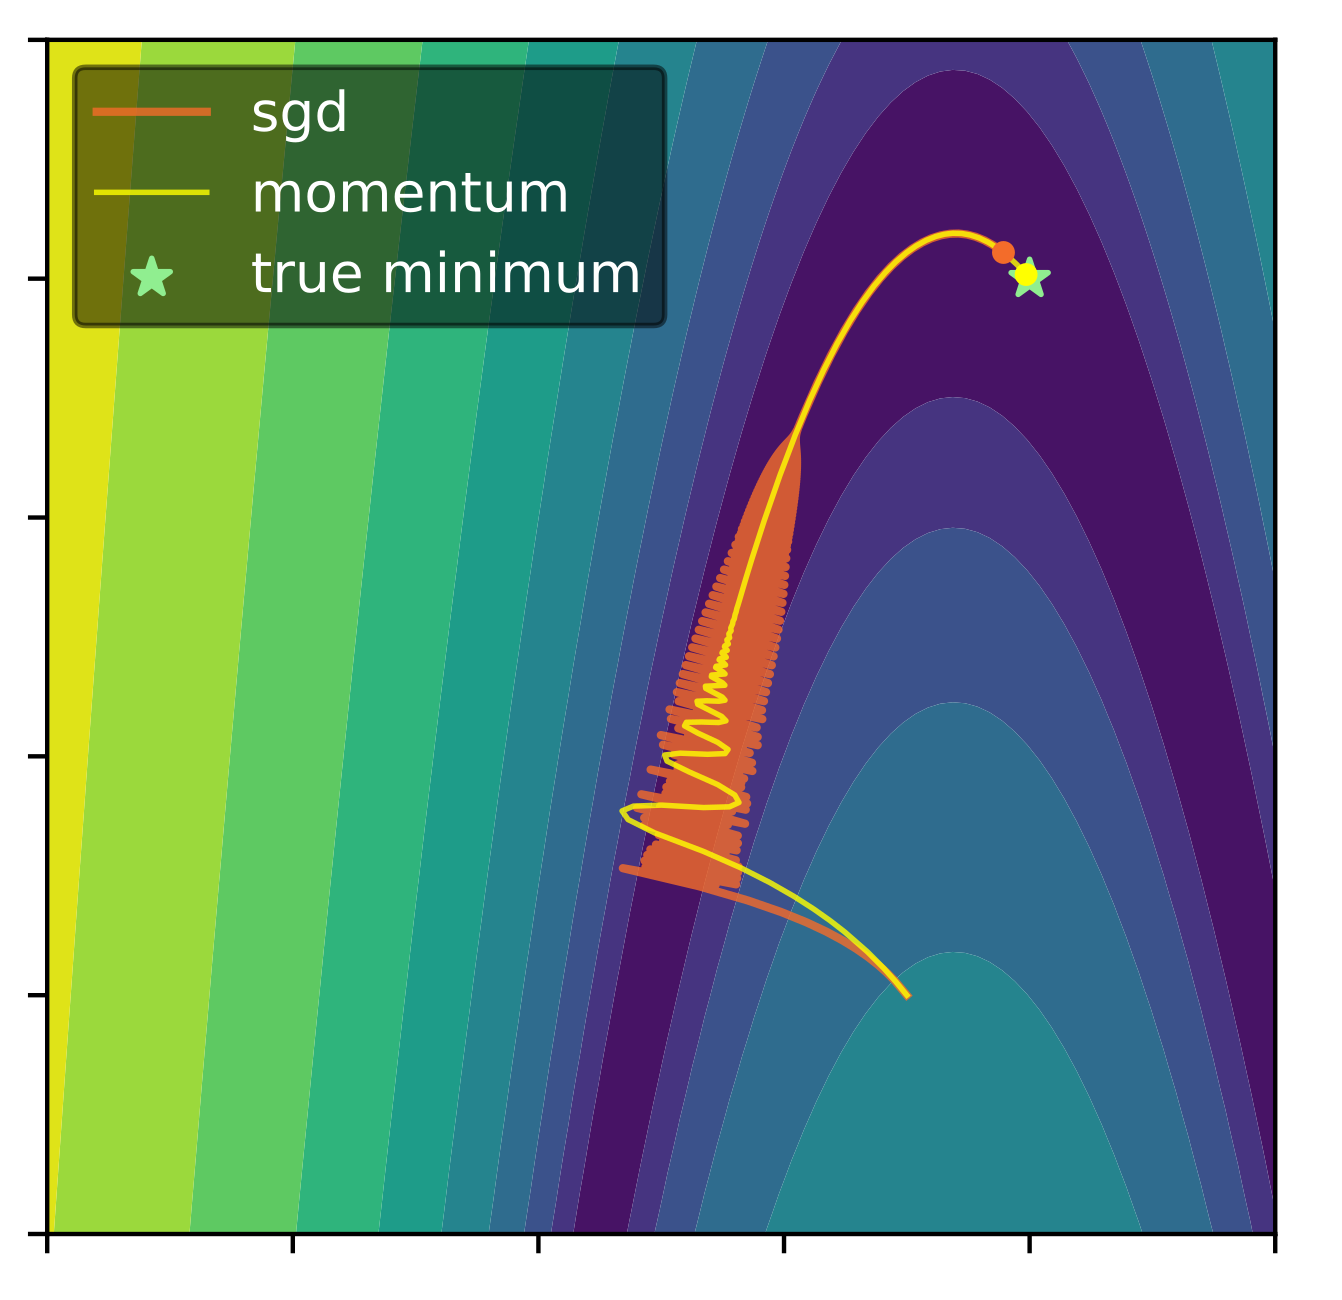
\includegraphics[width=.62\linewidth]{momentum}
	\end{textblock*}
	
	\begin{textblock*}{0.45\paperwidth}(0.62\paperwidth,0.72\paperheight)
		\includegraphics<2->[width=.75\linewidth]{nesterov}
	\end{textblock*}
\end{columns}

\begin{textblock*}{0.45\paperwidth}(0.7\paperwidth,0.1\paperheight)
	\footnotesize
	\textcolor{gray}{check out more on \href{https://distill.pub/2017/momentum/}{\underline{distill}}}
\end{textblock*}

\only<2->{\begin{textblock*}{0.45\paperwidth}(0.92\paperwidth,0.88\paperheight)
	\tiny
	\textcolor{gray}{\href{https://cs231n.github.io/neural-networks-3/}{\underline{source}}}
\end{textblock*}
}

\begin{textblock*}{0.45\paperwidth}(0.92\paperwidth,0.65\paperheight)
	\tiny
	\textcolor{gray}{\href{https://indico.cern.ch/event/838377/}{\underline{source}}}
\end{textblock*}

\end{frame}

%------------------------------------------------

\subsection{adaptive LR}
\begin{frame}

\myframetitle{0.4\paperwidth}{0.04\paperwidth}{\insertsection}
\myframesubtitle{0.41\paperwidth}{\insertsubsection}
\vspace{0.2\paperheight}
\begin{columns}
	\column{0.75\textwidth}
	\begin{itemize}
		\footnotesize
		\itemsep1.ex
		\setbeamertemplate{items}{\mybullet}
		\item<1-> Previously, we were manipulating learning rate $\eta$ \textbf{globally and equally} for all parameters
		\item<1-> This sounds like a limitation, since gradient scales vary significanty and we could've gained from adjusting LRs for \textbf{each component independently}
		\item<2-> So here comes \textcolor{gray}{\href{https://www.cs.toronto.edu/~tijmen/csc321/slides/lecture_slides_lec6.pdf}{\underline{RMSprop}}} (Hinton's lecture notes): 
		\[
			\text{\textbf{Var}}[g^2]_{(k)} \leftarrow \beta \cdot \text{\textbf{Var}}[g^2]_{(k-1)} + (1-\beta) \bigg(\dfrac{\partial Q}{\partial \bm \omega}\bigg)^2\bigg|_{\bm \omega = \bm \omega^{(k-1)}}
		\]
		\[
			\bm{\omega}^{(k)} \leftarrow \bm{\omega}^{(k-1)} - \dfrac{\eta}{\sqrt{\text{\textbf{Var}}[g^2]_{(k)} + \varepsilon}}\dfrac{\partial Q}{\partial \bm \omega}\bigg|_{\bm \omega = \bm \omega^{(k-1)}}
		\]
		\item<2-> \textcolor{gray}{\href{https://arxiv.org/abs/1412.6980}{\underline{\textbf{Adam}}}} combines ideas of momentum and RMSprop 
		\item<2->[] \textcolor{myorange}{Note:} there's also \textcolor{gray}{\href{https://www.jeremyjordan.me/nn-learning-rate/}{\underline{LR annealing}}} and \textcolor{gray}{\href{https://ruder.io/optimizing-gradient-descent/}{\underline{more sophisticated optimizers}}}
	\end{itemize}
	
	\column{0.5\textwidth}
	
	\begin{textblock*}{0.45\paperwidth}(0.65\paperwidth,0.22\paperheight)
		\includegraphics<2->[width=.75\linewidth]{optimizers}
	\end{textblock*}
	
%	\begin{textblock*}{0.45\paperwidth}(0.62\paperwidth,0.72\paperheight)
%		\includegraphics<2->[width=.75\linewidth]{nesterov}
%	\end{textblock*}
\end{columns}

\only<3->{

\begin{textblock*}{0.25\paperwidth}(0.7\paperwidth,0.82\paperheight)
	\centering 
	\footnotesize
	Nice moment to show \textcolor{gray}{\href{https://cs231n.github.io/neural-networks-3/\#ada}{\underline{this}}} animation
\end{textblock*}


}

\end{frame}

%------------------------------------------------

\subsection{weight regularisation}
\begin{frame}

\myframetitle{0.4\paperwidth}{0.04\paperwidth}{\insertsection}
\myframesubtitle{0.41\paperwidth}{\insertsubsection}

\vspace{0.23\paperheight}
\begin{columns}[t]
	\column{0.5\textwidth}
	\centering L2 regularization (Tikhonov)\\
	\vspace{1em}
	$Q(\bm{\omega})= \mathbb{E}_{\text{p}(\bm x,y)}\left[\mathcal{L}(y, f(\bm x, \bm \omega))\right] + \textcolor{myorange}{\lambda \sum\limits_{j=1}^{K}\bm\omega_j^2} $\\
	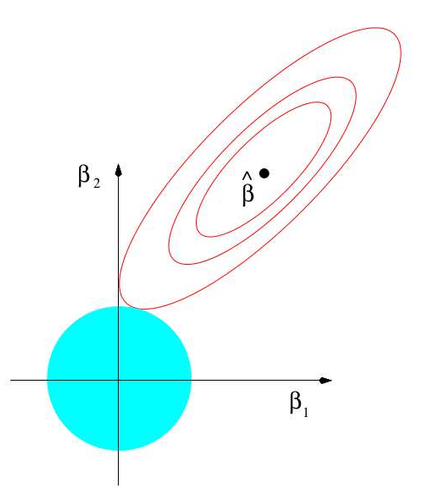
\includegraphics[width=0.4\linewidth]{ridge}\\
	
	\column{0.5\textwidth}
	\centering L1 regularization (LASSO)\\
	\vspace{-1mm}
	\tiny{\color{gray}least absolute shrinkage and selection operator}
	\normalsize
	\vspace{1mm}
	$Q(\bm{\omega})= \mathbb{E}_{\text{p}(\bm x,y)}\left[\mathcal{L}(y, f(\bm x, \bm \omega))\right] + \textcolor{myorange}{\lambda \sum\limits_{j=1}^{K}|\bm\omega_j|} $\\
	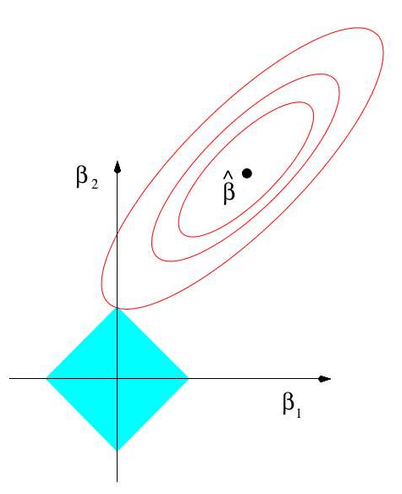
\includegraphics[width=0.4\linewidth]{lasso}
\end{columns}

	\begin{textblock*}{0.45\paperwidth}(0.81\paperwidth,0.65\paperheight)
		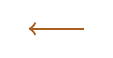
\begin{tikzpicture}
		\draw [->, myorange, thick] (0, 0) -- (-.7, .0);
		\end{tikzpicture}
	\end{textblock*}
	
	\begin{textblock*}{0.15\paperwidth}(0.87\paperwidth,0.63\paperheight)
		\scriptsize
		autozeroing uninformative weights!\\
%		\centering
%		$\downarrow$\\
%		\textcolor{mygreen}{
%			feature selection
%		}
	\end{textblock*}


\begin{textblock*}{0.45\paperwidth}(0.37\paperwidth,0.58\paperheight)
	\scriptsize
	penalize model for too large weights
\end{textblock*}

\begin{textblock*}{0.45\paperwidth}(0.6\paperwidth,0.45\paperheight)
	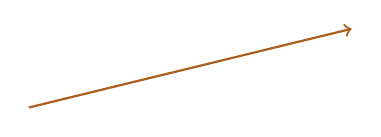
\begin{tikzpicture}
	\draw [->, myorange, thick] (0, 0) -- (4.1, 1.);
	\end{tikzpicture}
\end{textblock*}

\begin{textblock*}{0.45\paperwidth}(0.43\paperwidth,0.49\paperheight)
	
\begin{tikzpicture}
	\draw [->, myorange, thick] (0, 0) -- (.0, .7);
	\end{tikzpicture}
\end{textblock*}

%\begin{textblock*}{0.45\paperwidth}(0.55\paperwidth,0.1\paperheight)
%	\footnotesize
%	\textcolor{Gray}{playgrounds \href{https://developers.google.com/machine-learning/crash-course/regularization-for-simplicity/playground-exercise-examining-l2-regularization}{\underline{click}}, \href{https://developers.google.com/machine-learning/crash-course/regularization-for-sparsity/l1-regularization}{\underline{click}} }
%\end{textblock*}

\transfade[duration=.4]
\end{frame}

%------------------------------------------------

\subsection{dropout}
\begin{frame}

\myframetitle{0.4\paperwidth}{0.04\paperwidth}{\insertsection}
\myframesubtitle{0.41\paperwidth}{\insertsubsection}

\vspace{0.2\paperheight}

\begin{columns}
	\column{0.65\textwidth}
	\begin{itemize}
		\small
		\setbeamertemplate{items}{\mybullet}
		\item Let's randomly \textbf{drop neurons with probability $p$} during the training
		\item Essentially, this would mean that at each iteration we train a \textit{new subnetwork}
		\item This allows for \textbf{breaking co-adaptation} of neurons $\Rightarrow$ neurons forced to learn useful features w/o relying on neighbouring ones
		\item And makes it very simple, elegant and \textbf{powerful regularization} technique
		\item<2->[] \textcolor{myorange}{Note:} during testing one needs to simply scale neurons' outputs with $p$ to compensate \textit{on average} for dropout during the training
	\end{itemize}

	\column{0.45\textwidth}
	\begin{textblock*}{0.45\paperwidth}(0.62\paperwidth,0.25\paperheight)
		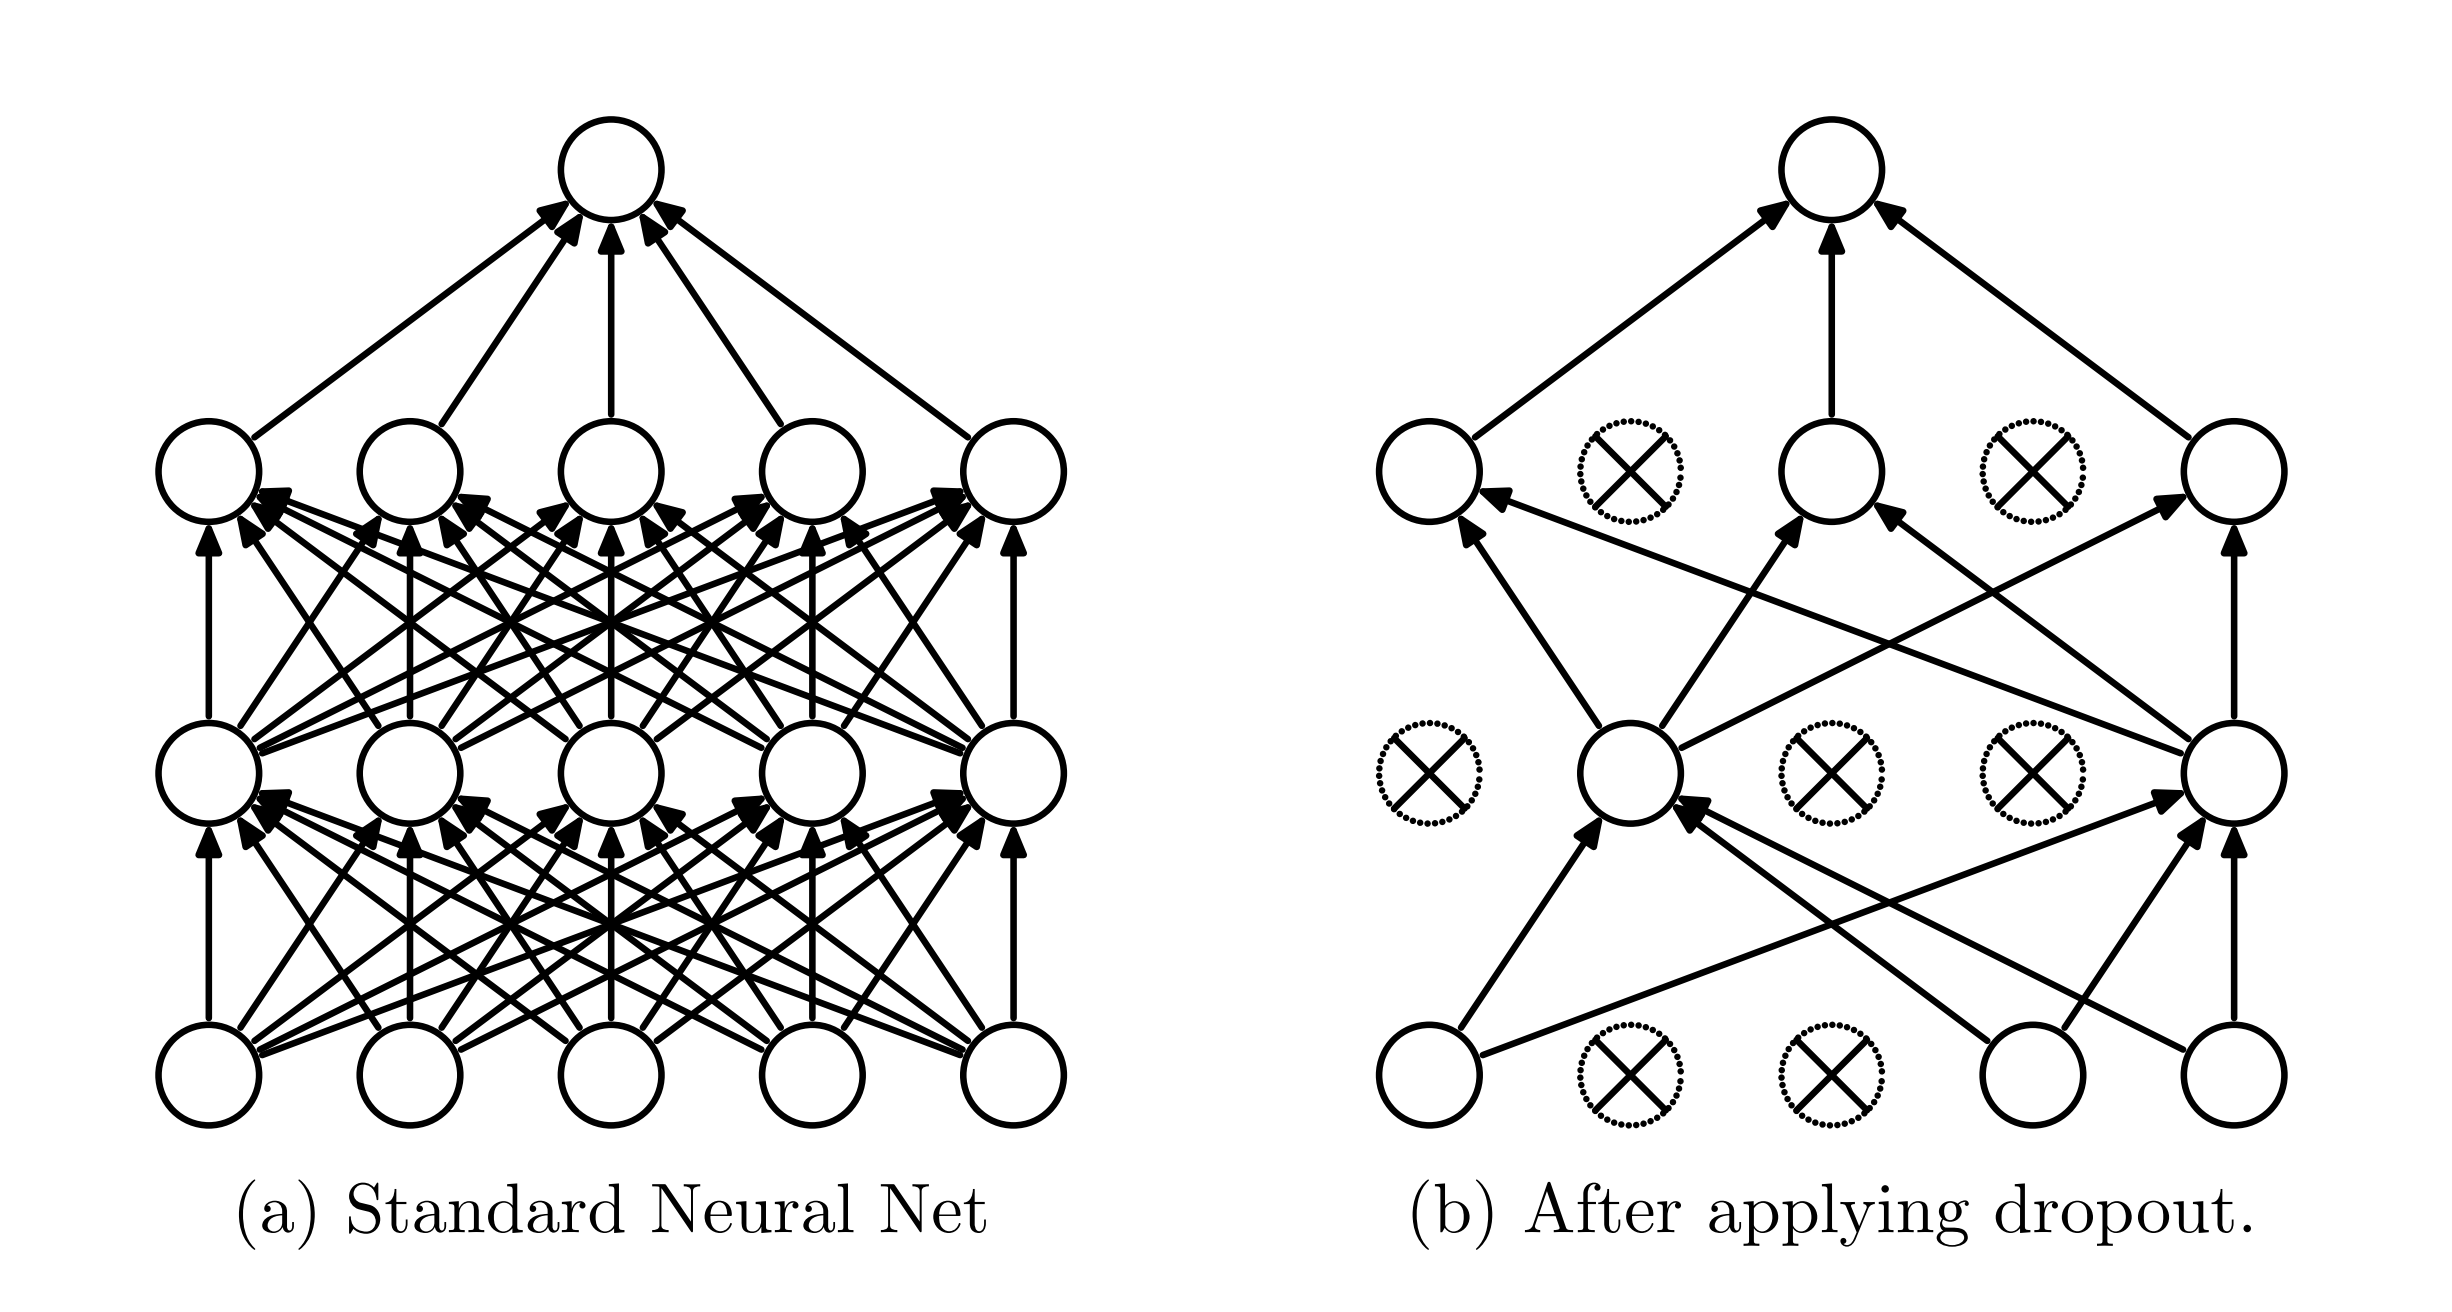
\includegraphics[width=.75\linewidth]{dropout_1}
	\end{textblock*}

	\begin{textblock*}{0.45\paperwidth}(0.62\paperwidth,0.61\paperheight)
		\includegraphics<2->[width=.75\linewidth]{dropout_2}
	\end{textblock*}
%	\includegraphics<2->[width=.9\linewidth]{dropout_2}
\end{columns}

\begin{textblock*}{0.45\paperwidth}(0.85\paperwidth,0.11\paperheight)
	\footnotesize
	\href{https://jmlr.org/papers/v15/srivastava14a.html}{\textcolor{gray}{\underline{paper}}}
\end{textblock*}

\end{frame}

%------------------------------------------------

\subsection{batch normalisation}
\begin{frame}

\myframetitle{0.4\paperwidth}{0.04\paperwidth}{\insertsection}
\myframesubtitle{0.41\paperwidth}{\insertsubsection}

\vspace{0.2\paperheight}

\begin{columns}
	\column{0.65\textwidth}
	\begin{itemize}
		\small 
		\setbeamertemplate{items}{\mybullet}
		\item As was mentioned earlier, training procedure is sensitive to the scale of gradients in NN
		\item Furthermore, the latter is connected to the inputs' scale of layers, which in turn tends to vary throughout the training (aka \textbf{"internal covariate shift"})
		\item This slows down the training and makes the procedure sensitive to weight initialisation 
	\end{itemize}
	
	\column{0.45\textwidth}
	
	\begin{textblock*}{0.45\paperwidth}(0.58\paperwidth,0.25\paperheight)
		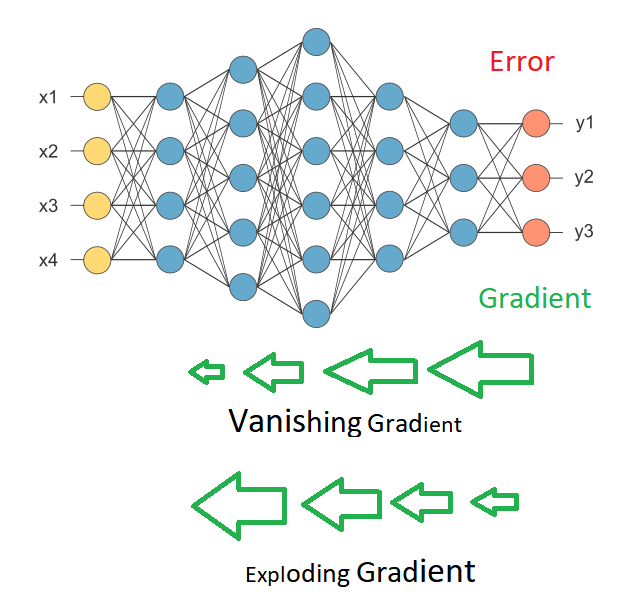
\includegraphics[width=.75\linewidth]{unstable_grad_NN}
	\end{textblock*}
%	
\end{columns}

\begin{textblock*}{0.45\paperwidth}(0.85\paperwidth,0.11\paperheight)
	\footnotesize
	\href{https://arxiv.org/abs/1502.03167}{\textcolor{gray}{\underline{paper}}}
\end{textblock*}

\end{frame}

%------------------------------------------------

\begin{frame}

\myframetitle{0.4\paperwidth}{0.04\paperwidth}{\insertsection}
\myframesubtitle{0.41\paperwidth}{\insertsubsection}

\vspace{0.2\paperheight}

\begin{columns}
	\column{0.65\textwidth}
	\begin{itemize}
		\small 
		\setbeamertemplate{items}{\mybullet}
		\item It was proposed to approach this problem with \textbf{normalising layer inputs} over a batch ($\gamma$ and $\beta$ are learnable parameters):
		\[
		\mu_B = \dfrac{1}{|B|}\sum\limits_{i \in B} x_i, \quad \sigma_B^2 = \dfrac{1}{|B|}\sum\limits_{i \in B} (x_i - \mu_B)^2
		\]
		\[
		y_i = \gamma\dfrac{x_i-\mu_B}{\sqrt{\sigma_B^2 + \epsilon}} + \beta
		\]
		\item This turned out to improve performance, speed up and stabilize convergence  (but \textcolor{gray}{\href{https://arxiv.org/pdf/1805.11604.pdf}{\underline{didn't really remove}}} internal covariate shift)
		\item[] \textcolor{myorange}{Note:} there are \textcolor{gray}{\href{https://arxiv.org/pdf/1803.08494.pdf}{\underline{other}}} fancy ways to normalize inputs
%		\item Effectively, it helps the model to \textbf{learn the required layers' mean and variance} through $\gamma$ and $\beta$
	\end{itemize}
	
	\column{0.45\textwidth}
	\begin{textblock*}{0.45\paperwidth}(0.62\paperwidth,0.25\paperheight)
		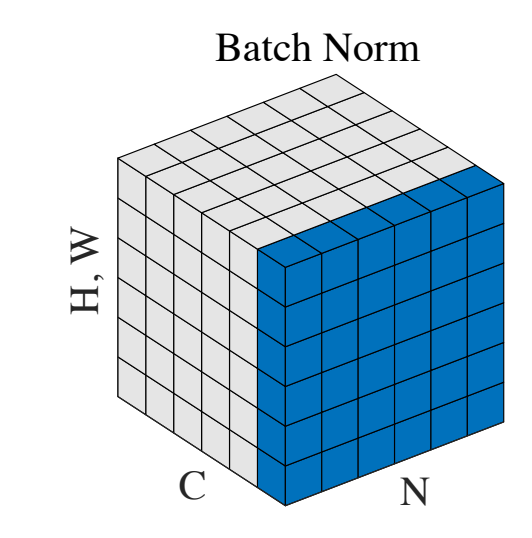
\includegraphics[width=.6\linewidth]{bn}
	\end{textblock*}
	
	%	\includegraphics<2->[width=.9\linewidth]{dropout_2}
\end{columns}

\begin{textblock*}{0.45\paperwidth}(0.85\paperwidth,0.11\paperheight)
	\footnotesize
	\href{https://arxiv.org/abs/1502.03167}{\textcolor{gray}{\underline{paper}}}
\end{textblock*}

\end{frame}

%------------------------------------------------
%------------------------------------------------
\section{NN zoo}
%------------------------------------------------
%------------------------------------------------


\begin{frame}[plain]
\centering
\huge

%\begin{textblock*}{0.3\paperwidth}(0.25\paperwidth,0.3\paperheight)
\centering
\vspace{0.1\paperheight}
\begin{tcolorbox}[colframe=white, colback=mygrey, width=0.3\paperwidth,
	arc=2.mm, boxsep=2mm,
	box align=center,
	halign=center,
	valign=center,
	]
	\insertsection
\end{tcolorbox}

%\end{textblock*}

\transfade[duration=.4]
\end{frame}

%------------------------------------------------

\begin{frame}

\centering
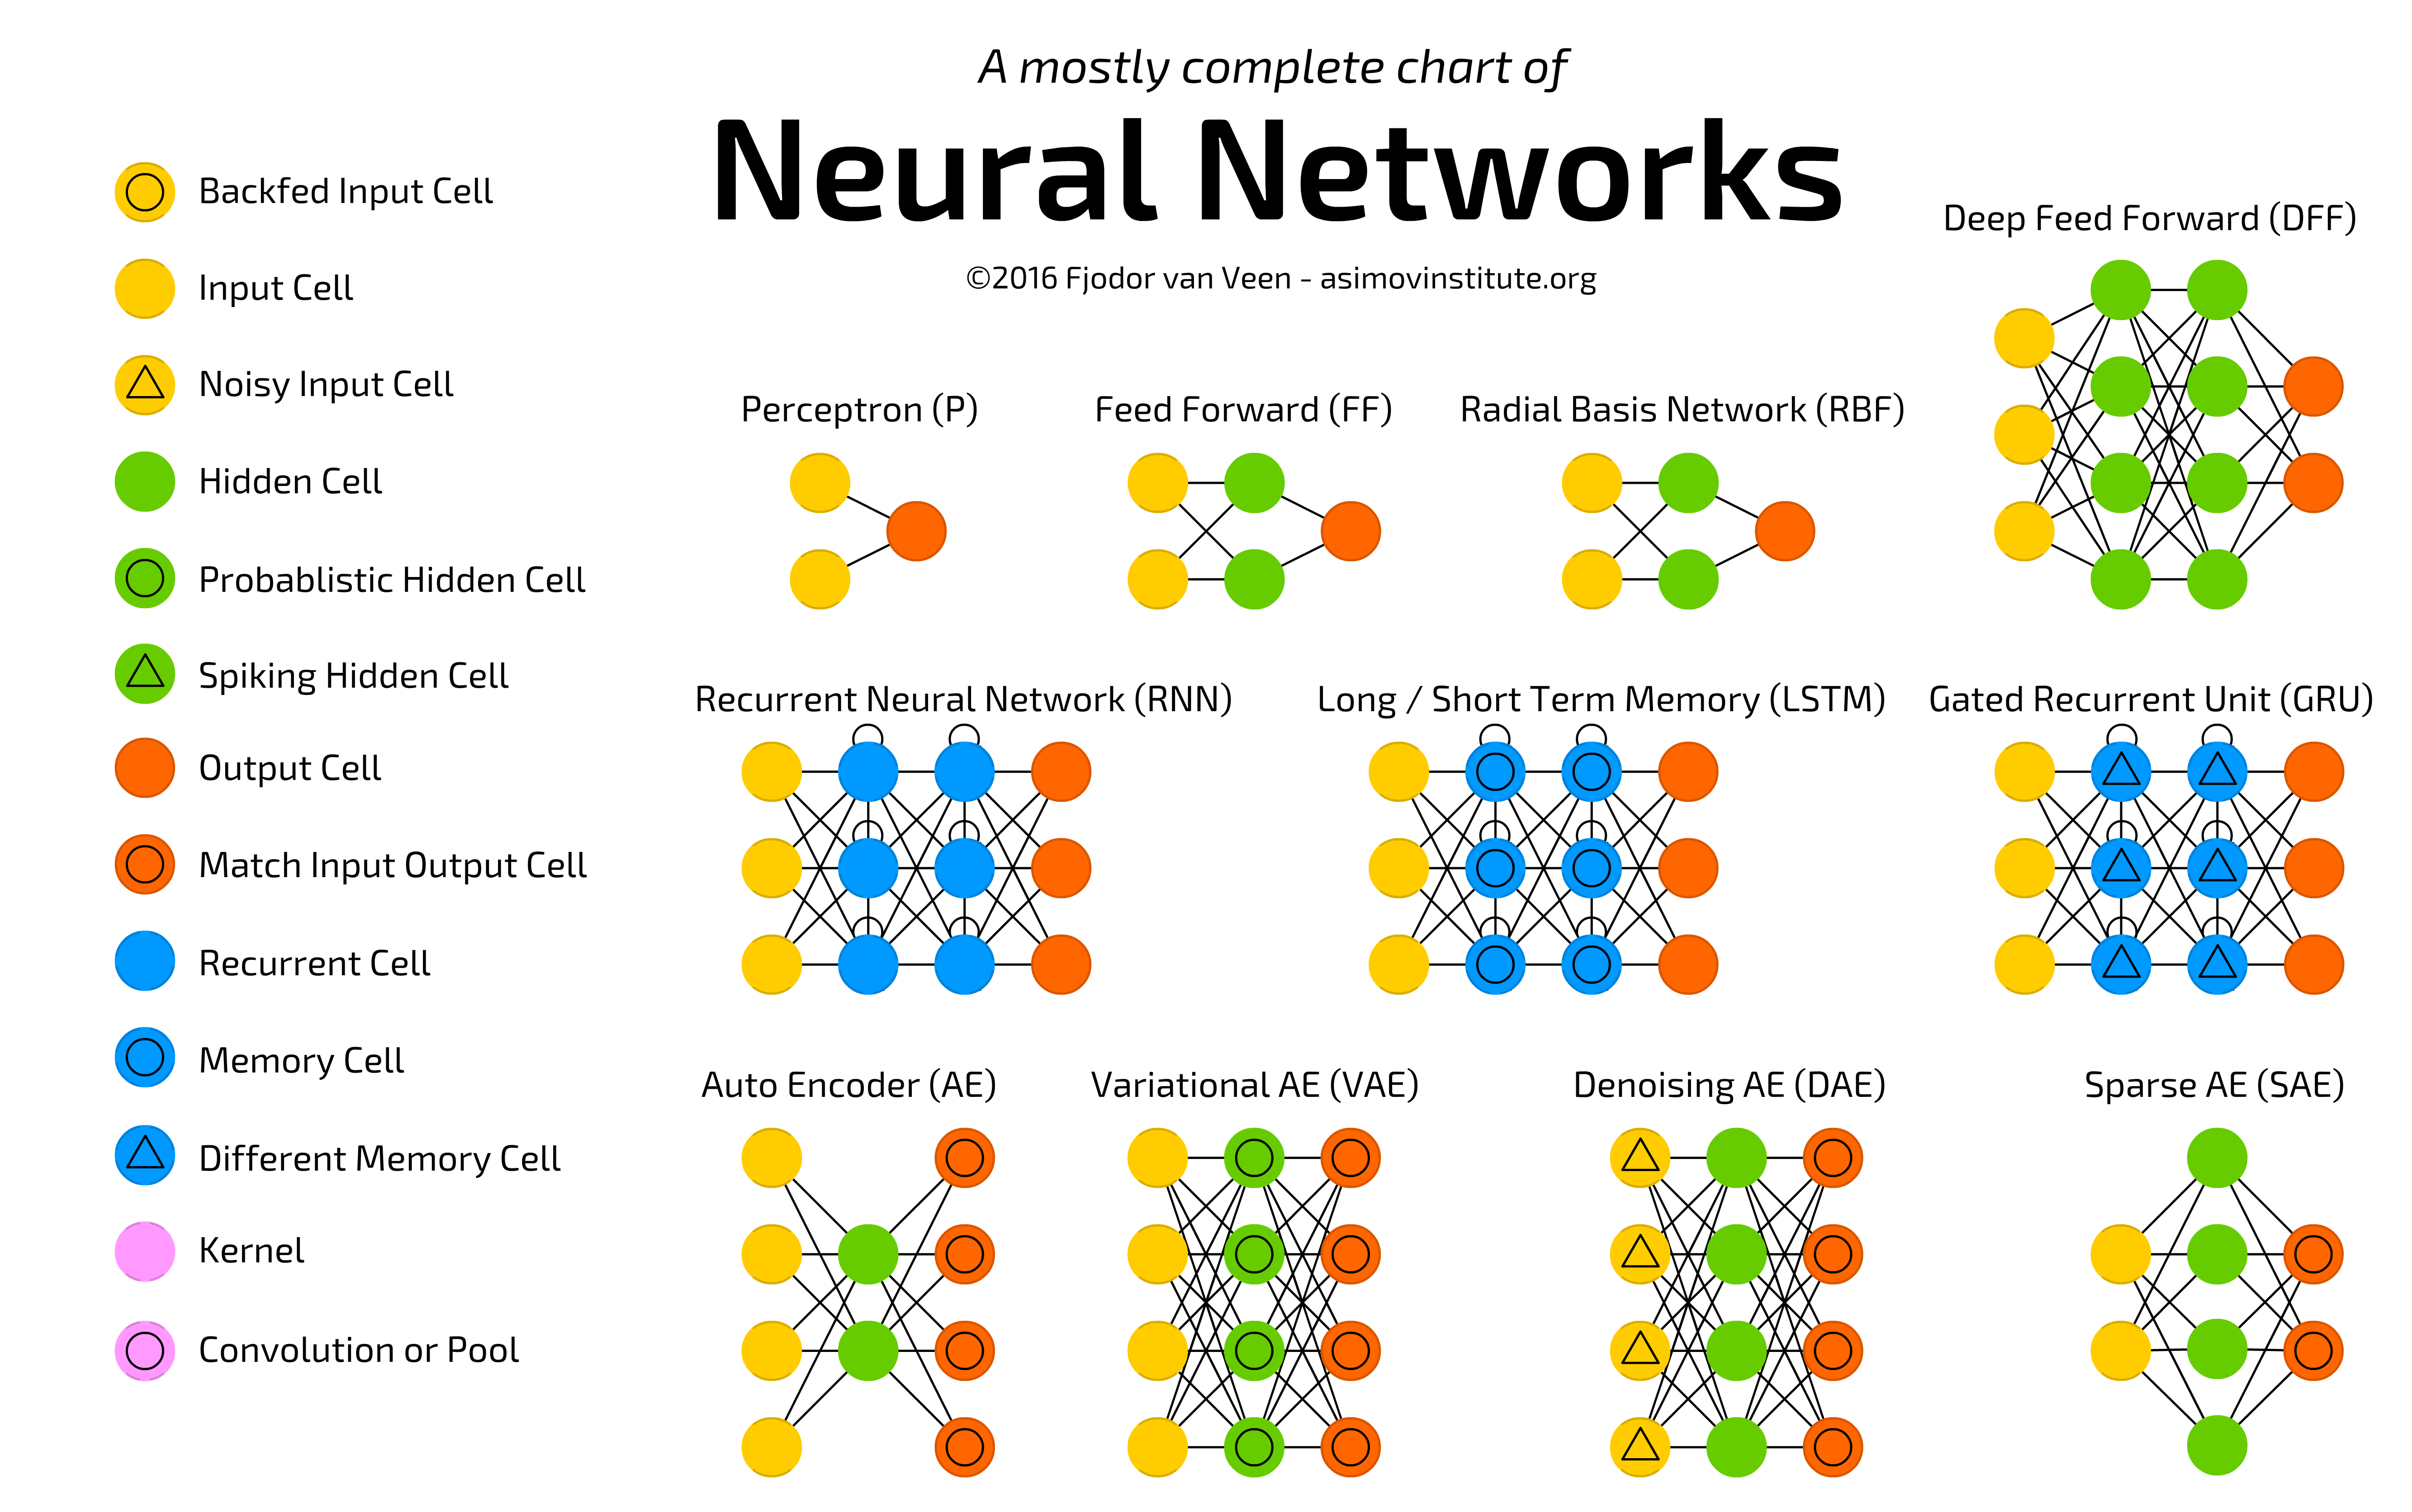
\includegraphics[width=0.85\linewidth]{networkZooPoster_1}

\begin{textblock*}{0.1\paperwidth}(0.87\paperwidth,0.07\paperheight)
	\footnotesize
	\href{https://www.asimovinstitute.org/neural-network-zoo/}{\textcolor{gray}{\underline{link}}}
\end{textblock*}


\end{frame}

%%------------------------------------------------
%
%\begin{frame}
%
%\centering
%%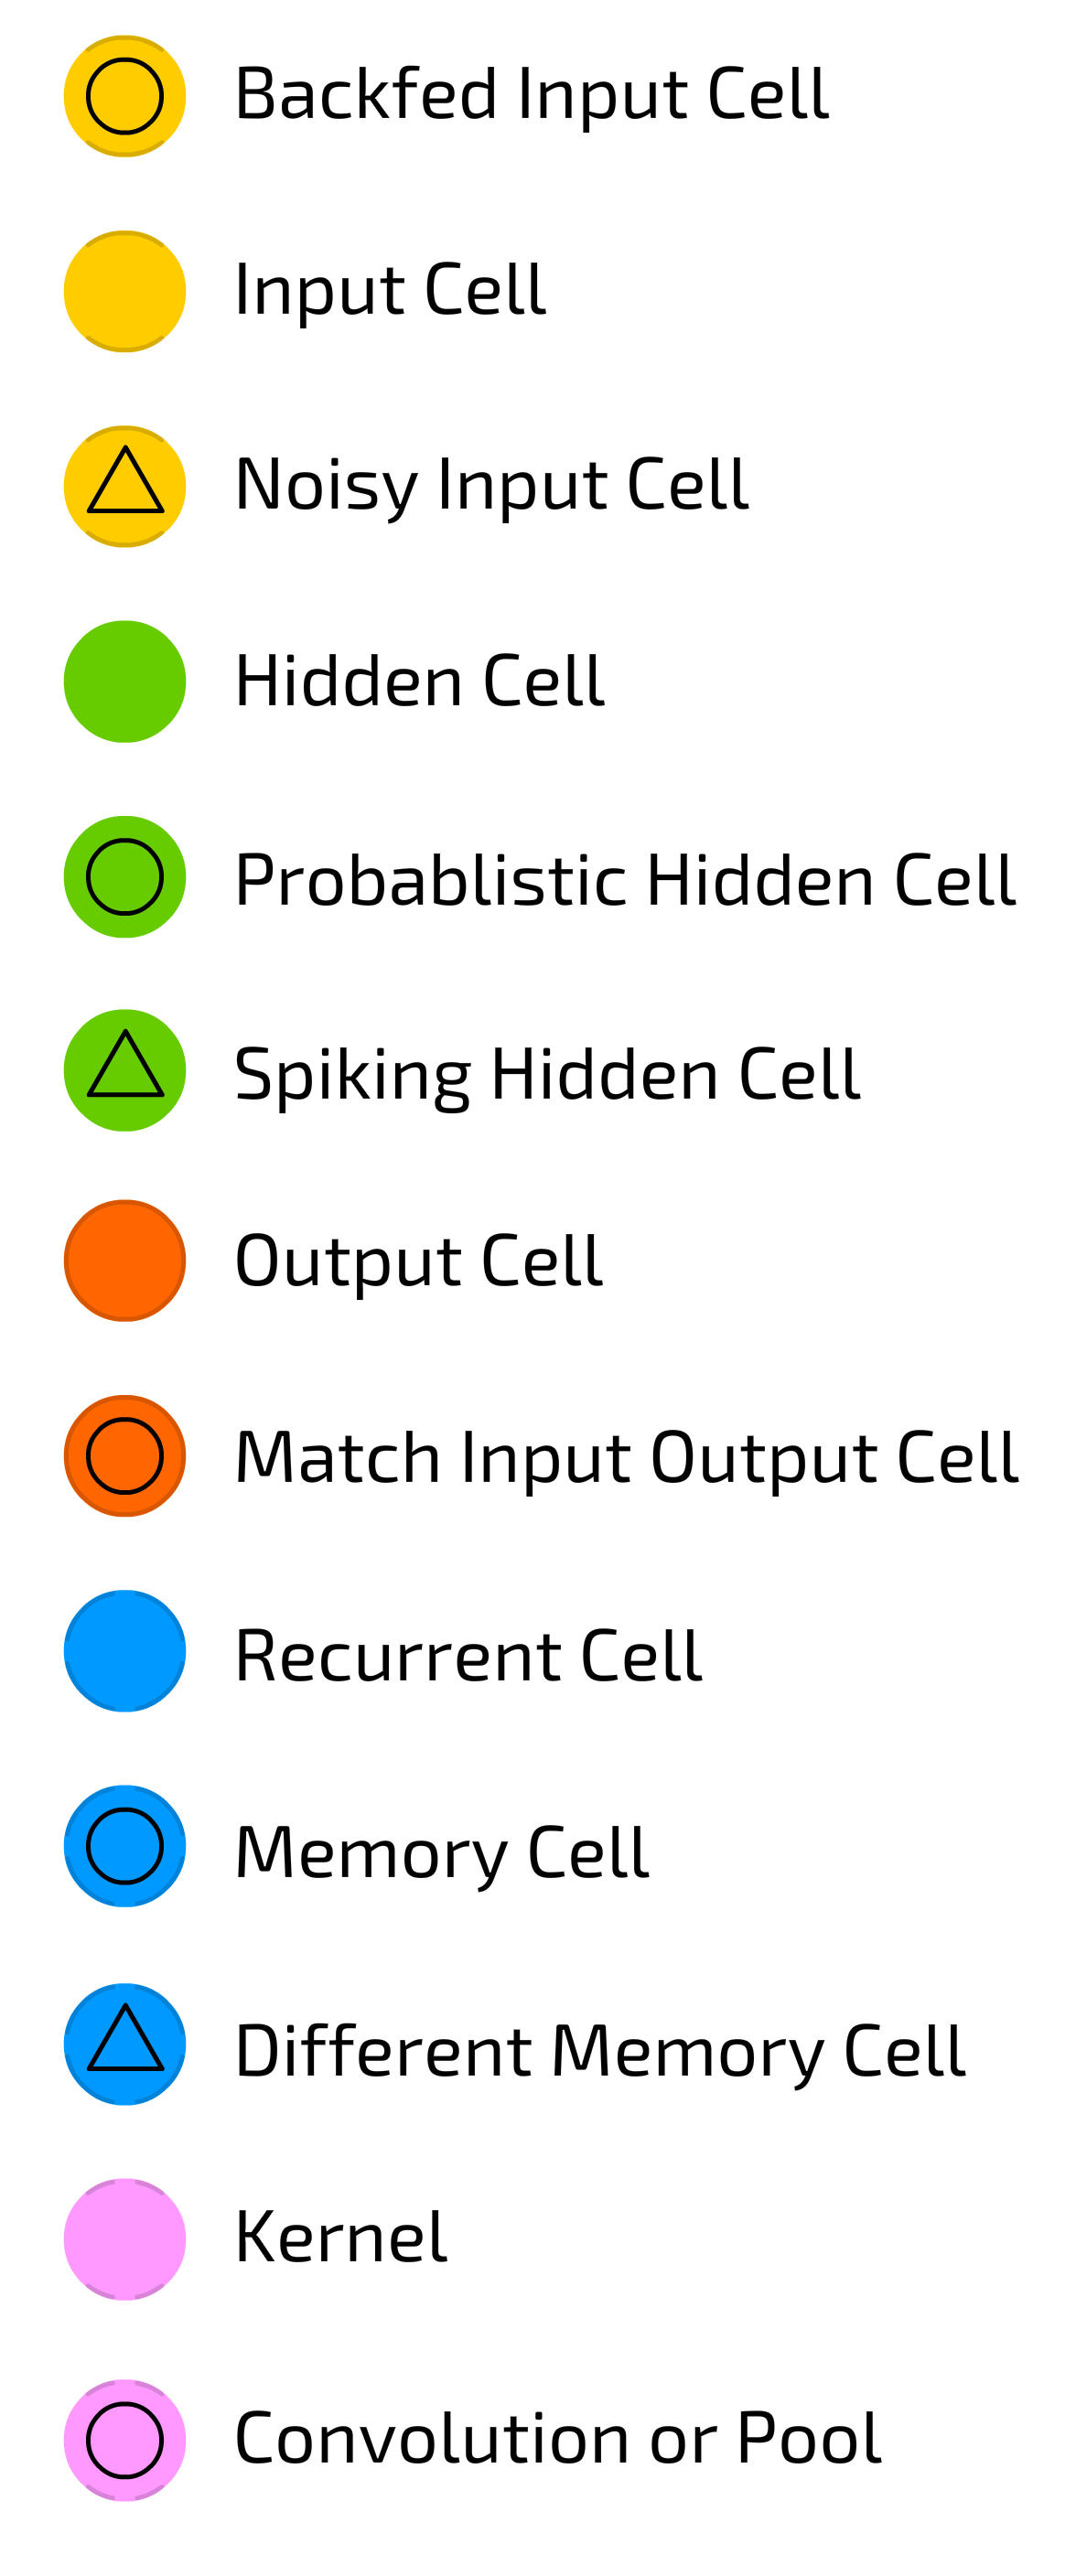
\includegraphics[width=0.1\linewidth]{networkZooPoster_leg}
%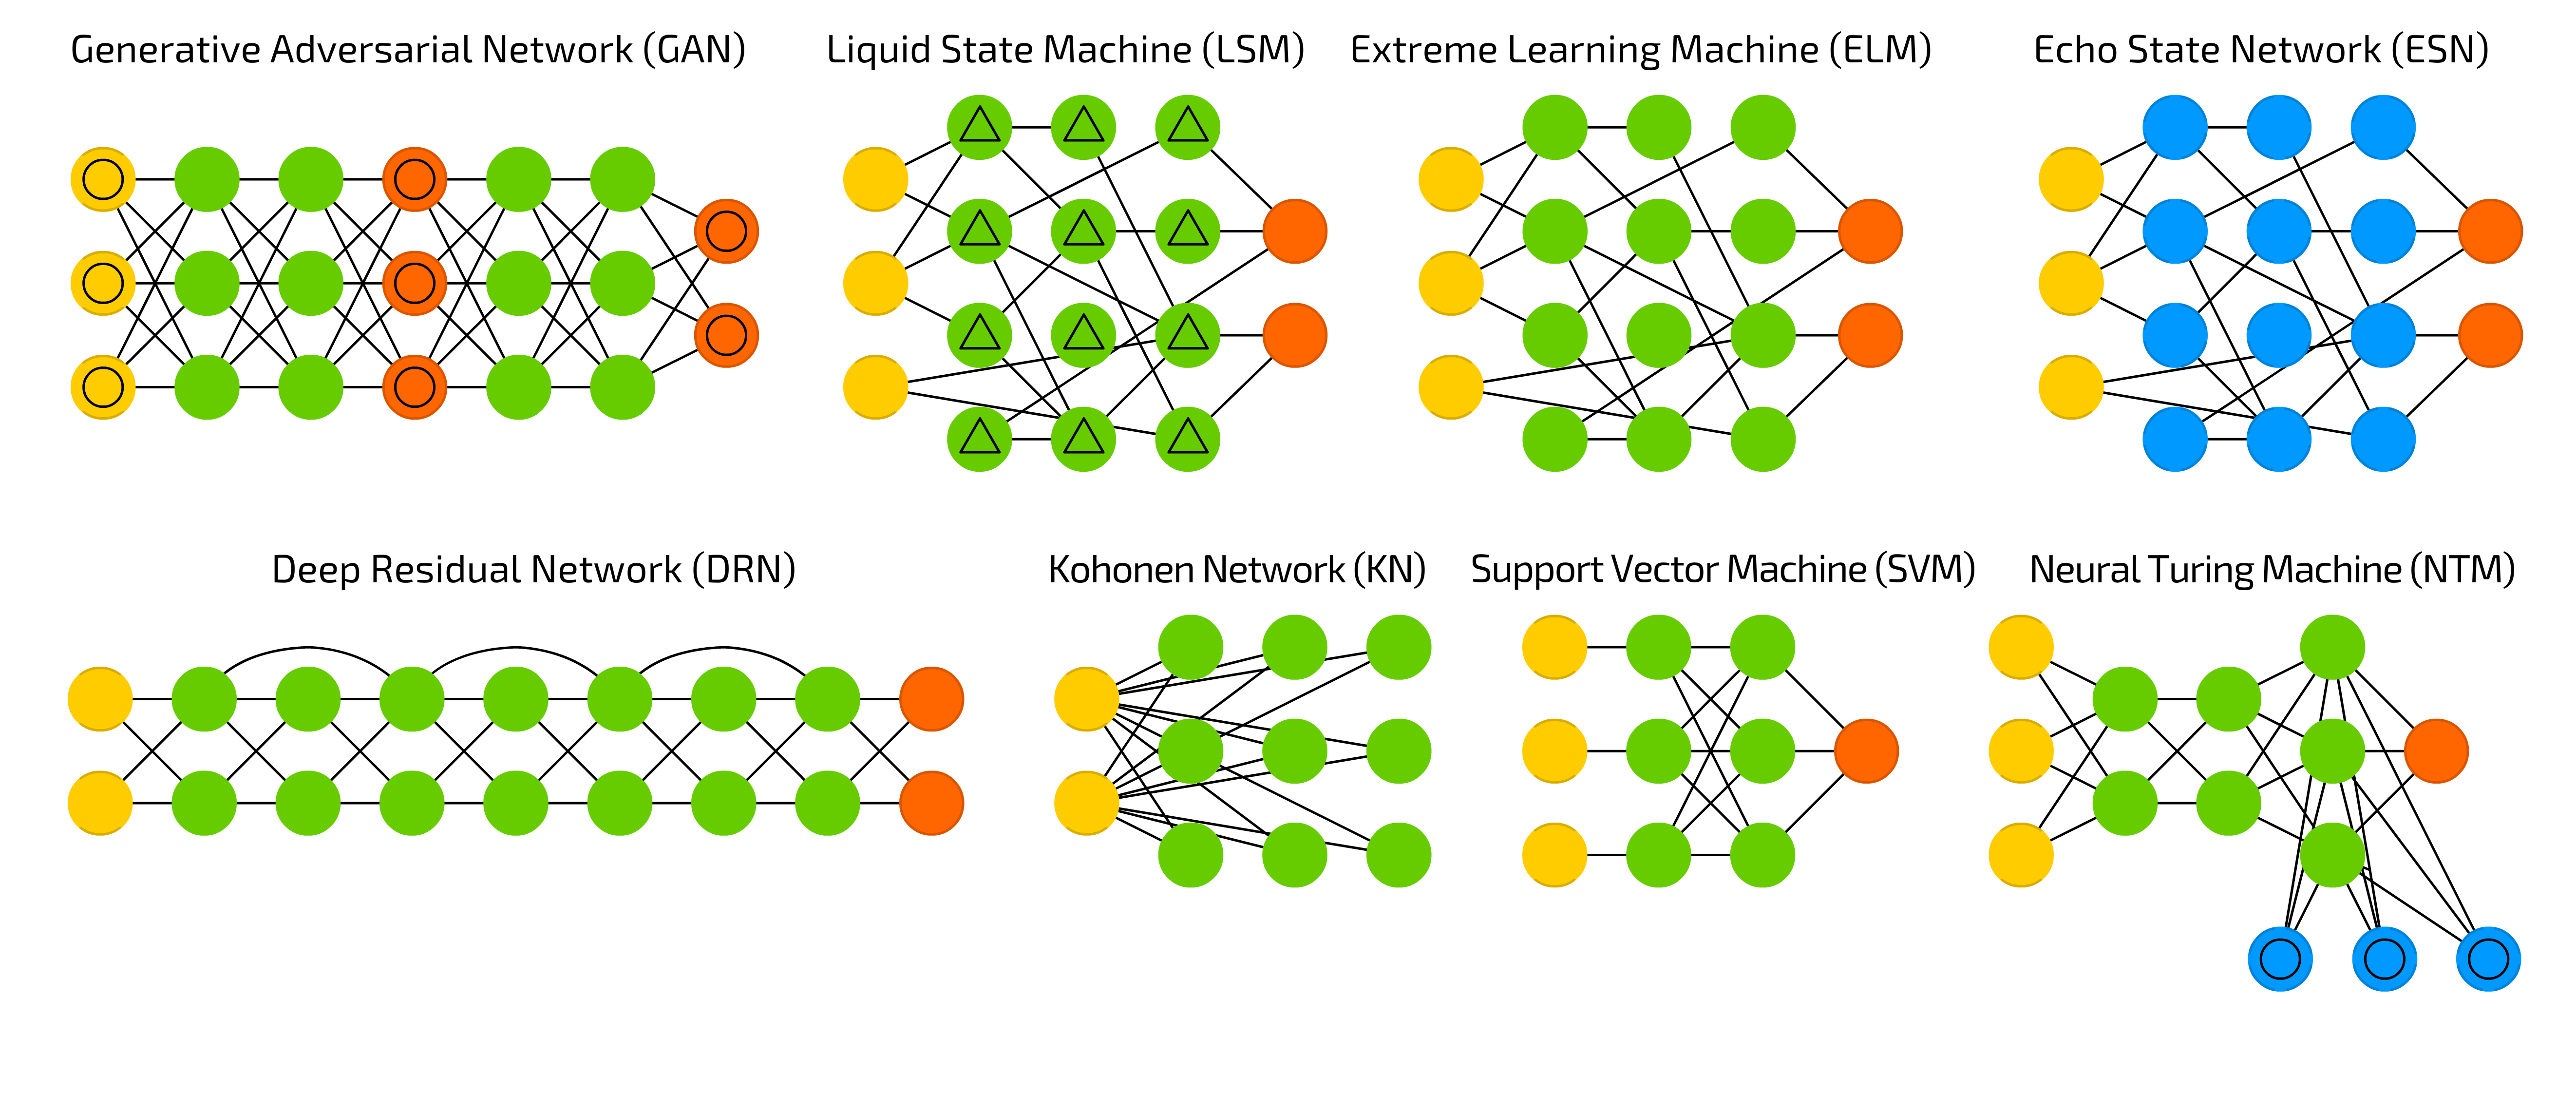
\includegraphics[width=0.85\linewidth]{networkZooPoster_3}
%
%\end{frame}

%------------------------------------------------
%------------------------------------------------
\section{Summary}
%------------------------------------------------
%------------------------------------------------

\begin{frame}

\myframetitle{0.25\paperwidth}{0.04\paperwidth}{\insertsection}
%\myframesubtitle{0.41\paperwidth}{\insertsubsection}

\vspace{0.2\paperheight}
\begin{columns}
	\column{0.5\textwidth}
	\begin{itemize}
		\itemsep0.8ex
		\setbeamertemplate{items}{\mybullet}
		\item Modelling nonlinearities
		\item Neural Network
		\begin{itemize}
			\footnotesize
			\itemsep0.5ex
			\setbeamertemplate{items}{\mysubbullet}
			\item automating feature engineering
			\item architecture
			\item terminology		
		\end{itemize}
		\item Training
		\begin{itemize}
			\footnotesize
			\itemsep0.5ex
			\setbeamertemplate{items}{\mysubbullet}
			\item chain rule
			\item backpropogation
		\end{itemize}
	\end{itemize}
	
	\column{0.5\textwidth}
	\begin{itemize}
		\itemsep0.8ex
		\setbeamertemplate{items}{\mybullet}
		\item Going deeper
		\begin{itemize}
			\footnotesize
			\itemsep0.5ex
			\setbeamertemplate{items}{\mysubbullet}
			\item universal approximation theorem
			\item vanishing gradients
			\item activation functions
			\item weight initialisation
		\end{itemize}
		\item Tackling overfitting
		\begin{itemize}
			\footnotesize
			\itemsep0.5ex
			\setbeamertemplate{items}{\mysubbullet}
			\item gradient descent modifications
			\item weight regularization
			\item dropout
			\item batch normalisation
		\end{itemize} 
		\item NN zoo
	\end{itemize}
\end{columns}

\end{frame}

%------------------------------------------------

\end{document}

